\documentclass[10pt,xcolor=table]{beamer}

\usetheme[progressbar=frametitle]{metropolis}
\usepackage{appendixnumberbeamer}
\usepackage{hyperref}
\usepackage{tikz}
% \usetikzlibrary{calc,decorations.pathreplacing,snakes}
\usetikzlibrary{calc,decorations.pathreplacing}
\usepackage{multicol}
\usepackage{comment}
% \usepackage[portuguese]{babel}
% \usepackage[style=authortitle,backend=bibtex]{biblatex}
\usepackage[style=authortitle,backend=biber]{biblatex}
\addbibresource{references.bib}
\usepackage{subfig}
\usepackage{csquotes}
\usepackage{caption}
\usepackage{listings}

% Define style for C code
\lstdefinestyle{CStyle}{
  language=C,
  basicstyle=\ttfamily\footnotesize,
  keywordstyle=\color{blue},
  stringstyle=\color{red},
  commentstyle=\color{green!50!black},
  showstringspaces=false,
  breaklines=true,
  frame=single,
  numbers=left,
  numberstyle=\tiny\color{gray},
  tabsize=2
}

\hypersetup{colorlinks=true,linkcolor=,urlcolor=blue}

\expandafter\def\expandafter\insertshorttitle\expandafter{%
  \insertshorttitle\hfill%
  \insertframenumber\,/\,\inserttotalframenumber}

\newcommand{\hideFromPandoc}[1]{#1}
\hideFromPandoc{
  \let\Begin\begin
  \let\End\end
}

\newcommand{\verbatimfont}[1]{\renewcommand{\verbatim@font}{\ttfamily#1}}

\newcommand{\PR}[1]{\ensuremath{\left[#1\right]}}
\newcommand{\PC}[1]{\ensuremath{\left(#1\right)}}
\newcommand{\chav}[1]{\ensuremath{\left\{#1\right\}}}

\usepackage{booktabs}
\usepackage[scale=2]{ccicons}

\usepackage{pgfpages} % for multiple-screen presentations
% \setbeameroption{show notes on second screen}
% \setbeameroption{show notes on second screen=right} % Both

\usepackage{pgfplots}
\usepgfplotslibrary{dateplot}

\usepackage{xspace}
\newcommand{\themename}{\textbf{\textsc{metropolis}}\xspace}


\setbeamertemplate{frame footer}{
\includegraphics[height=0.65cm]{figs/ifpb.png}}

\setbeamercolor{background canvas}{bg=white}

% \setbeamertemplate{sections/subsections in toc}[ball]
\setbeamertemplate{section in toc}[sections numbered]
\setbeamertemplate{subsection in toc}[ball unnumbered]
\setbeamerfont{footnote}{size=\scriptsize}

\setbeamertemplate{blocks}[rounded][shadow]
% \setbeameroption{show notes}

% \renewcommand{\footnotesize}{\small}
% \renewcommand*{\bibfont}{\tiny}

% Main slide
\title{Bachelor's Degree Program in \\ Software Engineering}
% \subtitle{Subtitle}
\date{\today}
% \date{October 31, 2024}
\author{\textbf{Prof. Dr. Paulo Ditarso Maciel Jr. (\href{mailto:paulo.maciel@ifpb.edu.br}{paulo.maciel@ifpb.edu.br})}}
\institute{
\centering
\normalsize
\vspace{0.5cm}
{\Large \textbf{Operating Systems}}\\
\vspace{1cm}
{\small \textbf{Based on material from the book \href{https://pages.cs.wisc.edu/~remzi/OSTEP/}{\textit{Operating Systems: Three Easy Pieces}}.}} \\
\vspace{1cm}
{\scriptsize
\texttt{\$ git clone \href{https://github.com/pdmjr/network_intro.git}{https://github.com/pdmjr/ostep\_slides.git}}
}
}

\titlegraphic{\hfill
\includegraphics[height=1.7cm]{figs/ifpb.png}}

% -----------------------------------------------------------------------------
% Figure placeholder used throughout this outline.
% Replace each placeholder with \includegraphics[width=...]{...} after extracting
% the corresponding figure from the chapter PDF.
% -----------------------------------------------------------------------------
\newcommand{\figureplaceholder}[2]{%
  \begin{center}
    \fbox{%
      \begin{minipage}[c][0.27\textheight][c]{0.88\linewidth}
        \centering
        \textbf{#1}\\[0.5em]
        \small #2
      \end{minipage}%
    }
  \end{center}
}

\begin{document}

\maketitle

% Slide de Aviso

\begin{frame}
    \frametitle{Disclaimer\footnote{All figures used in this presentation are publicly available on websites, scientific papers or are licensed under the \textit{Creative Commons}.}}
    \begin{itemize}
        \item This presentation is not intended to dive deeply into any topic.
        \item It is essential to read the books and materials provided!
        \item What is the purpose of this presentation?
    \end{itemize}
    \begin{figure}
        \centering
        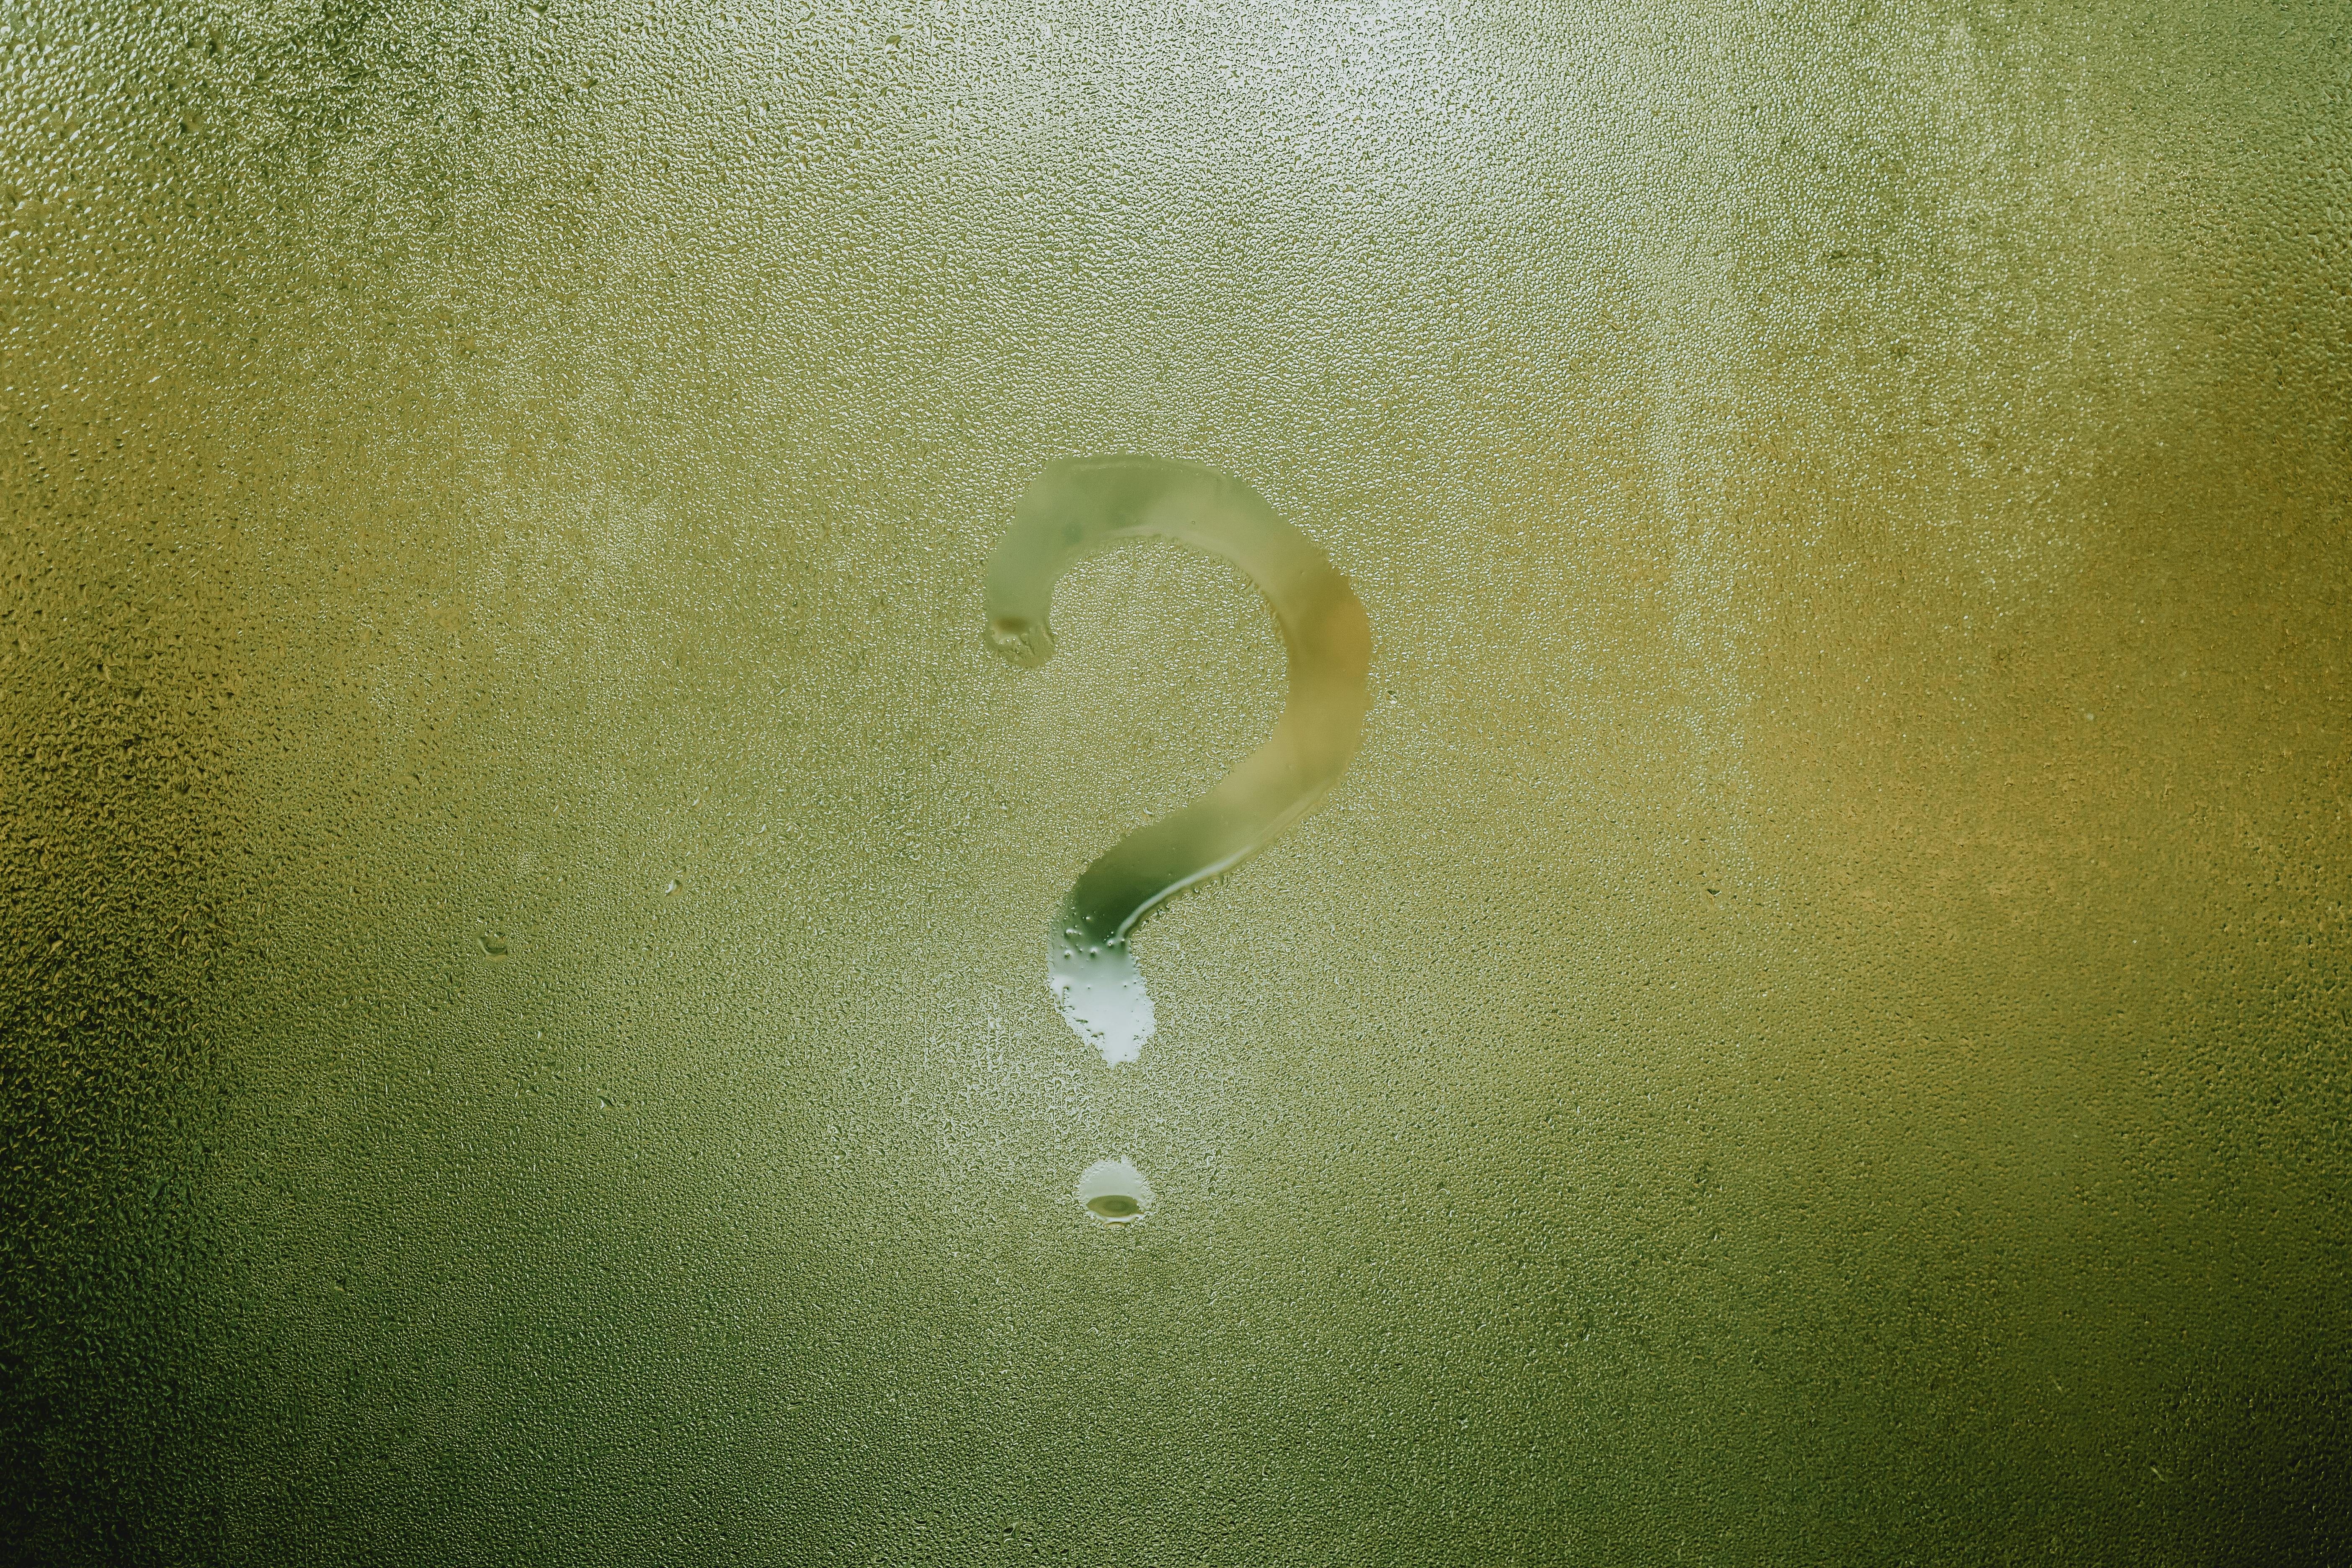
\includegraphics[width=0.6\textwidth]{figs/questionmark.jpg}
    \end{figure}
    \vspace{1cm}
\end{frame}

% Slide de Agenda
\begin{frame}
    \frametitle{Agenda}
    % \tableofcontents
    \begin{multicols}{2} % Altere para 3 se quiser três colunas
        \tableofcontents
    \end{multicols}
\end{frame}
% ---------------------------------------------------------
\section{A Dialogue on the Book}

% ---------------------------------------------------------
\begin{frame}{A Dialogue on the Book}

{\small
The dialogue introduces the book and explains the origin of its title, inspired by Richard Feynman's
\textit{Six Easy Pieces}.

\vspace{0.1cm}

The book is organized around three fundamental ideas:
\textbf{virtualization}, \textbf{concurrency}, and \textbf{persistence}.
Through these topics, it explores how operating systems manage processors, memory, storage, virtual machines, and even some aspects of distributed systems.

\vspace{0.1cm}

The dialogue also emphasizes an effective approach to learning operating
systems: attending classes, reviewing the material regularly, completing
homework, and especially developing projects that involve writing real code
to solve real problems.

\vspace{0.1cm}

Finally, the dialogue explains that these conversations are intended to
encourage reflection on complex concepts and help the reader reason about
the ideas presented throughout the book.
}

\end{frame}
\section{Introduction}

% Slide 1
\begin{frame}{What Happens When a Program Runs?}
  \begin{itemize}
    \item A running program executes instructions.
    \item The processor repeatedly \textbf{fetches}, \textbf{decodes}, and \textbf{executes} instructions.
    \item Programs assume an orderly, sequential execution model.
    \item The operating system works underneath this simple model to make the machine easier to use.
  \end{itemize}

  \vspace{0.5em}
  \begin{block}{Key idea}
    The OS hides much of the complexity involved in sharing and managing hardware resources.
  \end{block}
\end{frame}

% Slide 2
\begin{frame}{What Does an Operating System Do?}
  \begin{itemize}
    \item Makes it easier to run programs and use hardware resources.
    \item \textbf{Virtualizes} physical resources such as the CPU, memory, and storage.
    \item Provides interfaces through \textbf{system calls}.
    \item Acts as a \textbf{resource manager} for shared system resources.
  \end{itemize}

  \vspace{0.5em}
  \begin{alertblock}{The Crux of the Problem}
    How does the operating system virtualize resources efficiently, and what hardware support is needed?
  \end{alertblock}

  % Source location: shaded ``Crux of the Problem'' box, chapter page 2.
\end{frame}

% Slide 3
\begin{frame}{Virtualizing the CPU}
  \begin{columns}[T,onlytextwidth]
    \column{0.48\textwidth}
      \begin{itemize}
        \item The example program repeatedly waits and prints a user-provided string.
        \item A single program running alone is straightforward.
        \item The interesting behavior appears when several copies execute at once.
      \end{itemize}

    \column{0.50\textwidth}
    \begin{figure}
        \centering
        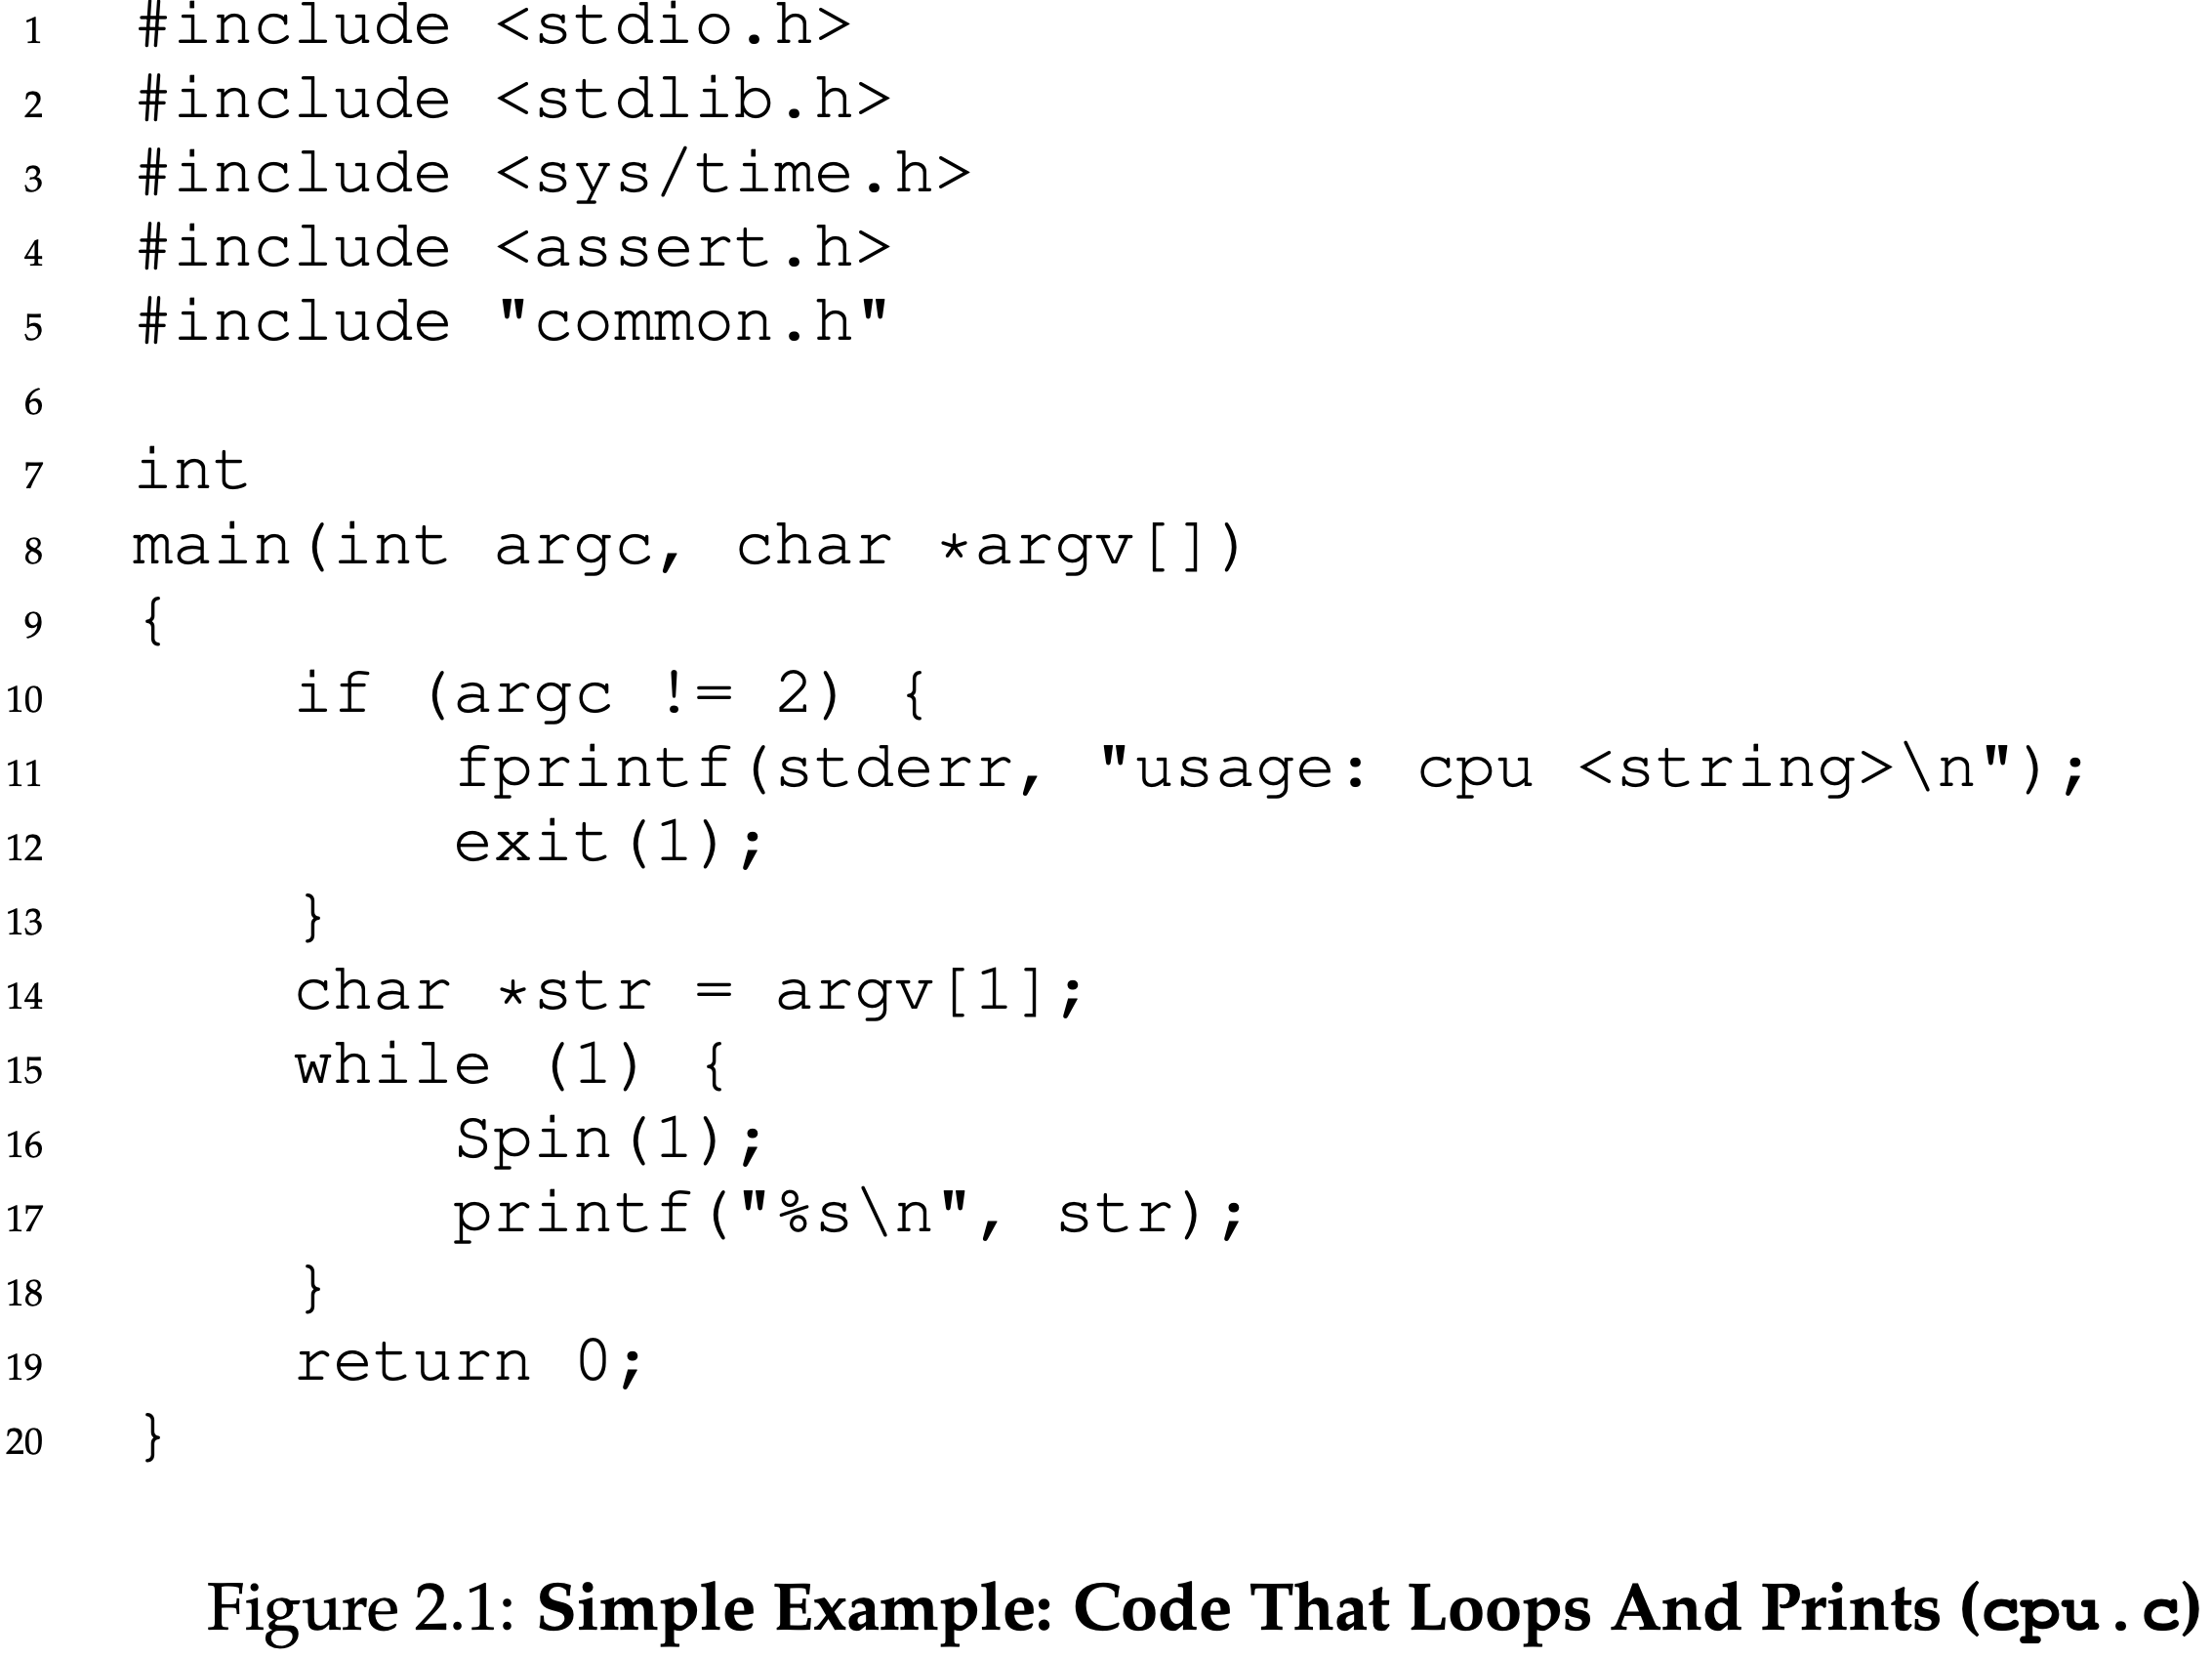
\includegraphics[width=1.1\linewidth]{figs/chapter-2/figure-2.1.png}
        \caption*{Source: chapter page 3.}
        \label{fig:figure-2.1}
    \end{figure}
      % \figureplaceholder{Figure 2.1: cpu.c}{Place the book figure here. Source: chapter page 3.}
  \end{columns}
\end{frame}

% Slide 4
\begin{frame}{The Illusion of Many CPUs}
  \begin{columns}[T,onlytextwidth]
    \column{0.48\textwidth}
    \begin{figure}
        \centering
        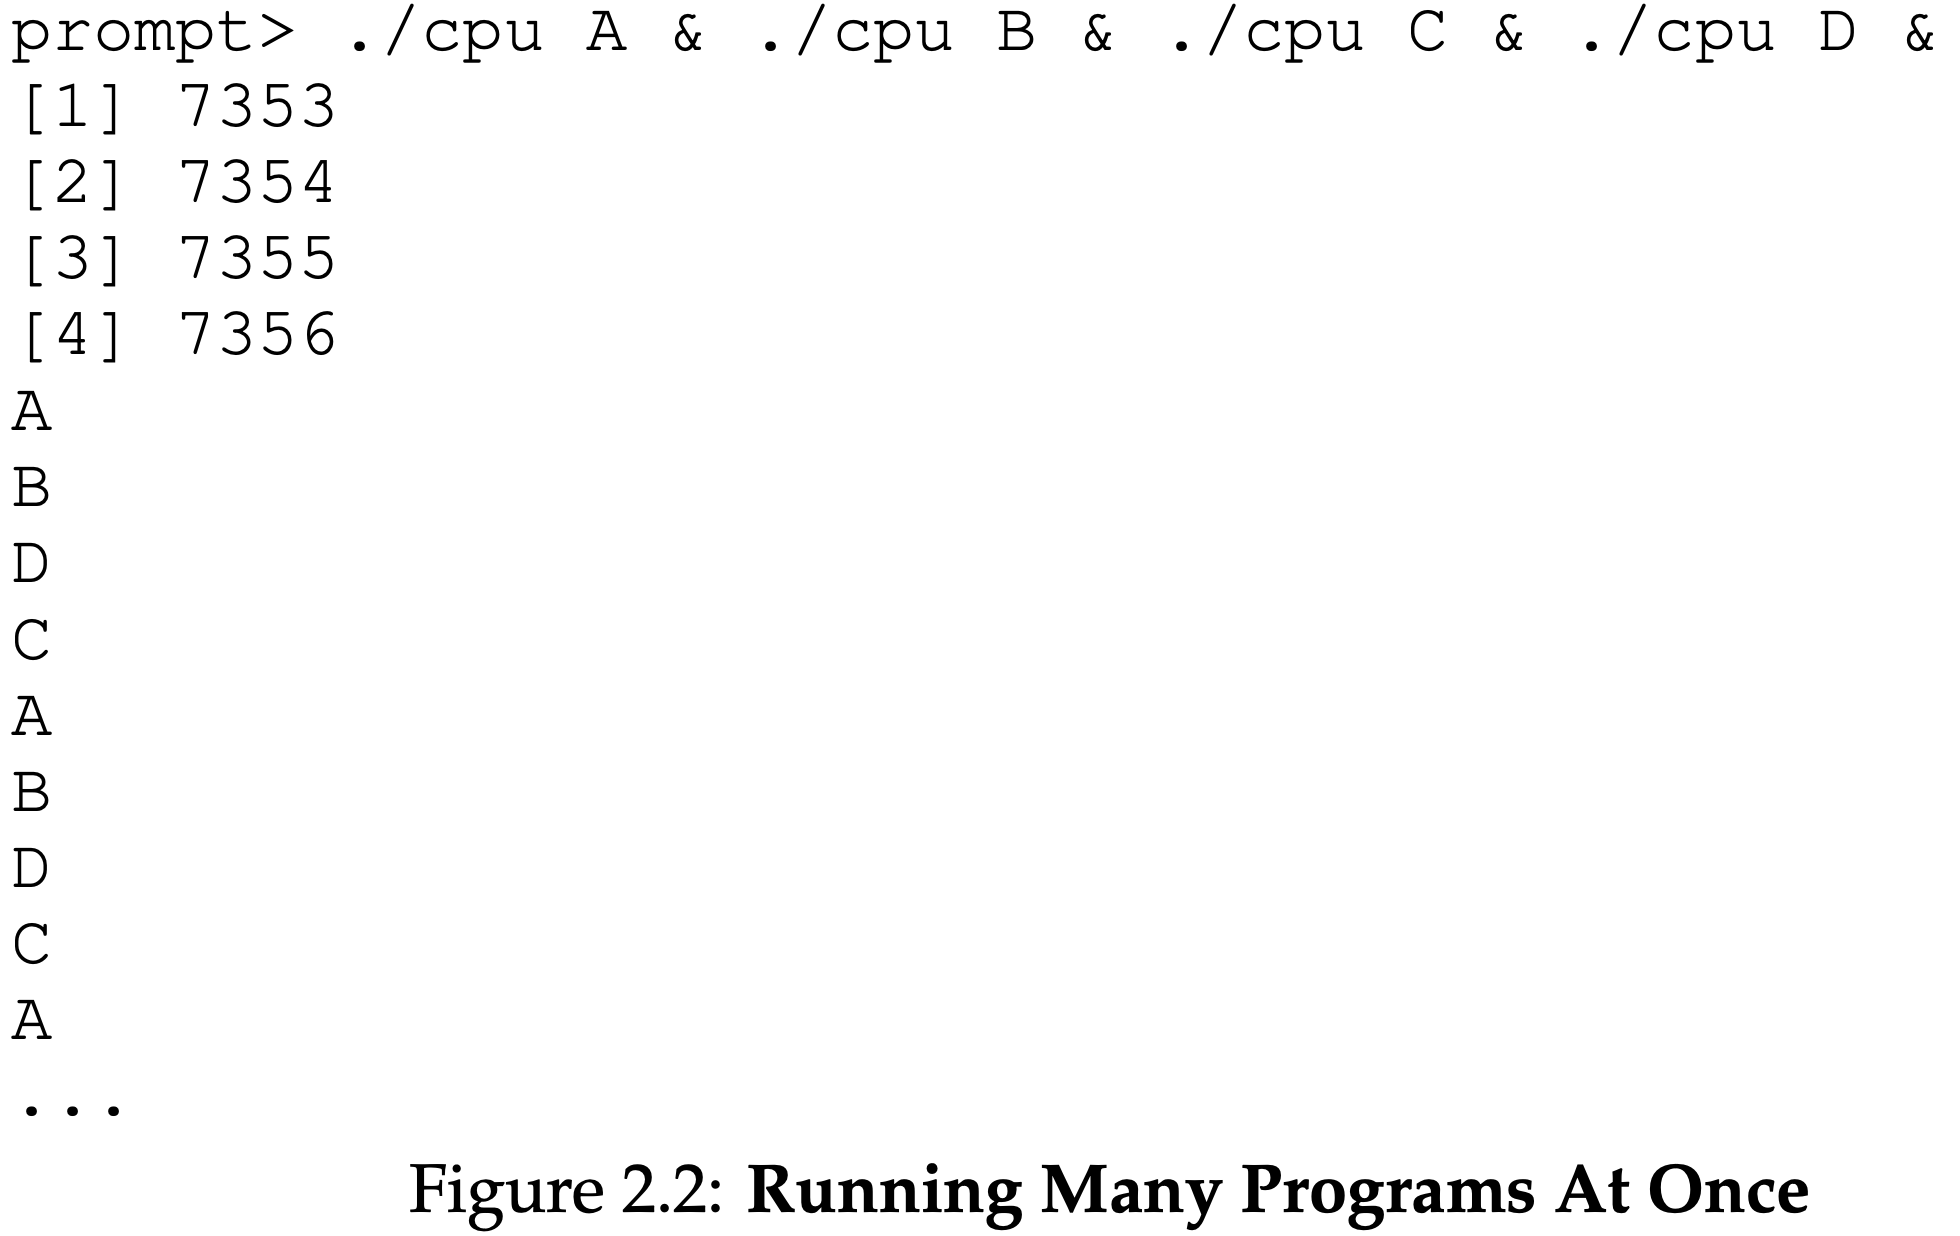
\includegraphics[width=1.1\linewidth]{figs/chapter-2/figure-2.2.png}
        \caption*{Source: chapter page 4.}
        \label{fig:figure-2.2}
    \end{figure}
      % \figureplaceholder{Figure 2.2: Running Many Programs At Once}{Place the book figure here. Source: chapter page 4.}

    \column{0.50\textwidth}
      \begin{itemize}
        \item Multiple programs appear to run simultaneously even on one processor.
        \item The OS, with hardware support, creates the illusion of many \textbf{virtual CPUs}.
        \item The OS also needs policies to decide which program should run at a given time.
      \end{itemize}
  \end{columns}
\end{frame}

% Slide 5
\begin{frame}{Virtualizing Memory}
  \begin{columns}[T,onlytextwidth]
    \column{0.48\textwidth}
      \begin{itemize}
        \item Memory can be viewed as an array of bytes addressed by the processor.
        \item Programs continuously access memory for instructions and data.
        \item The example allocates memory with \texttt{malloc()}, initializes it, and repeatedly updates it.
      \end{itemize}

    \column{0.50\textwidth}
    \begin{figure}
        \centering
        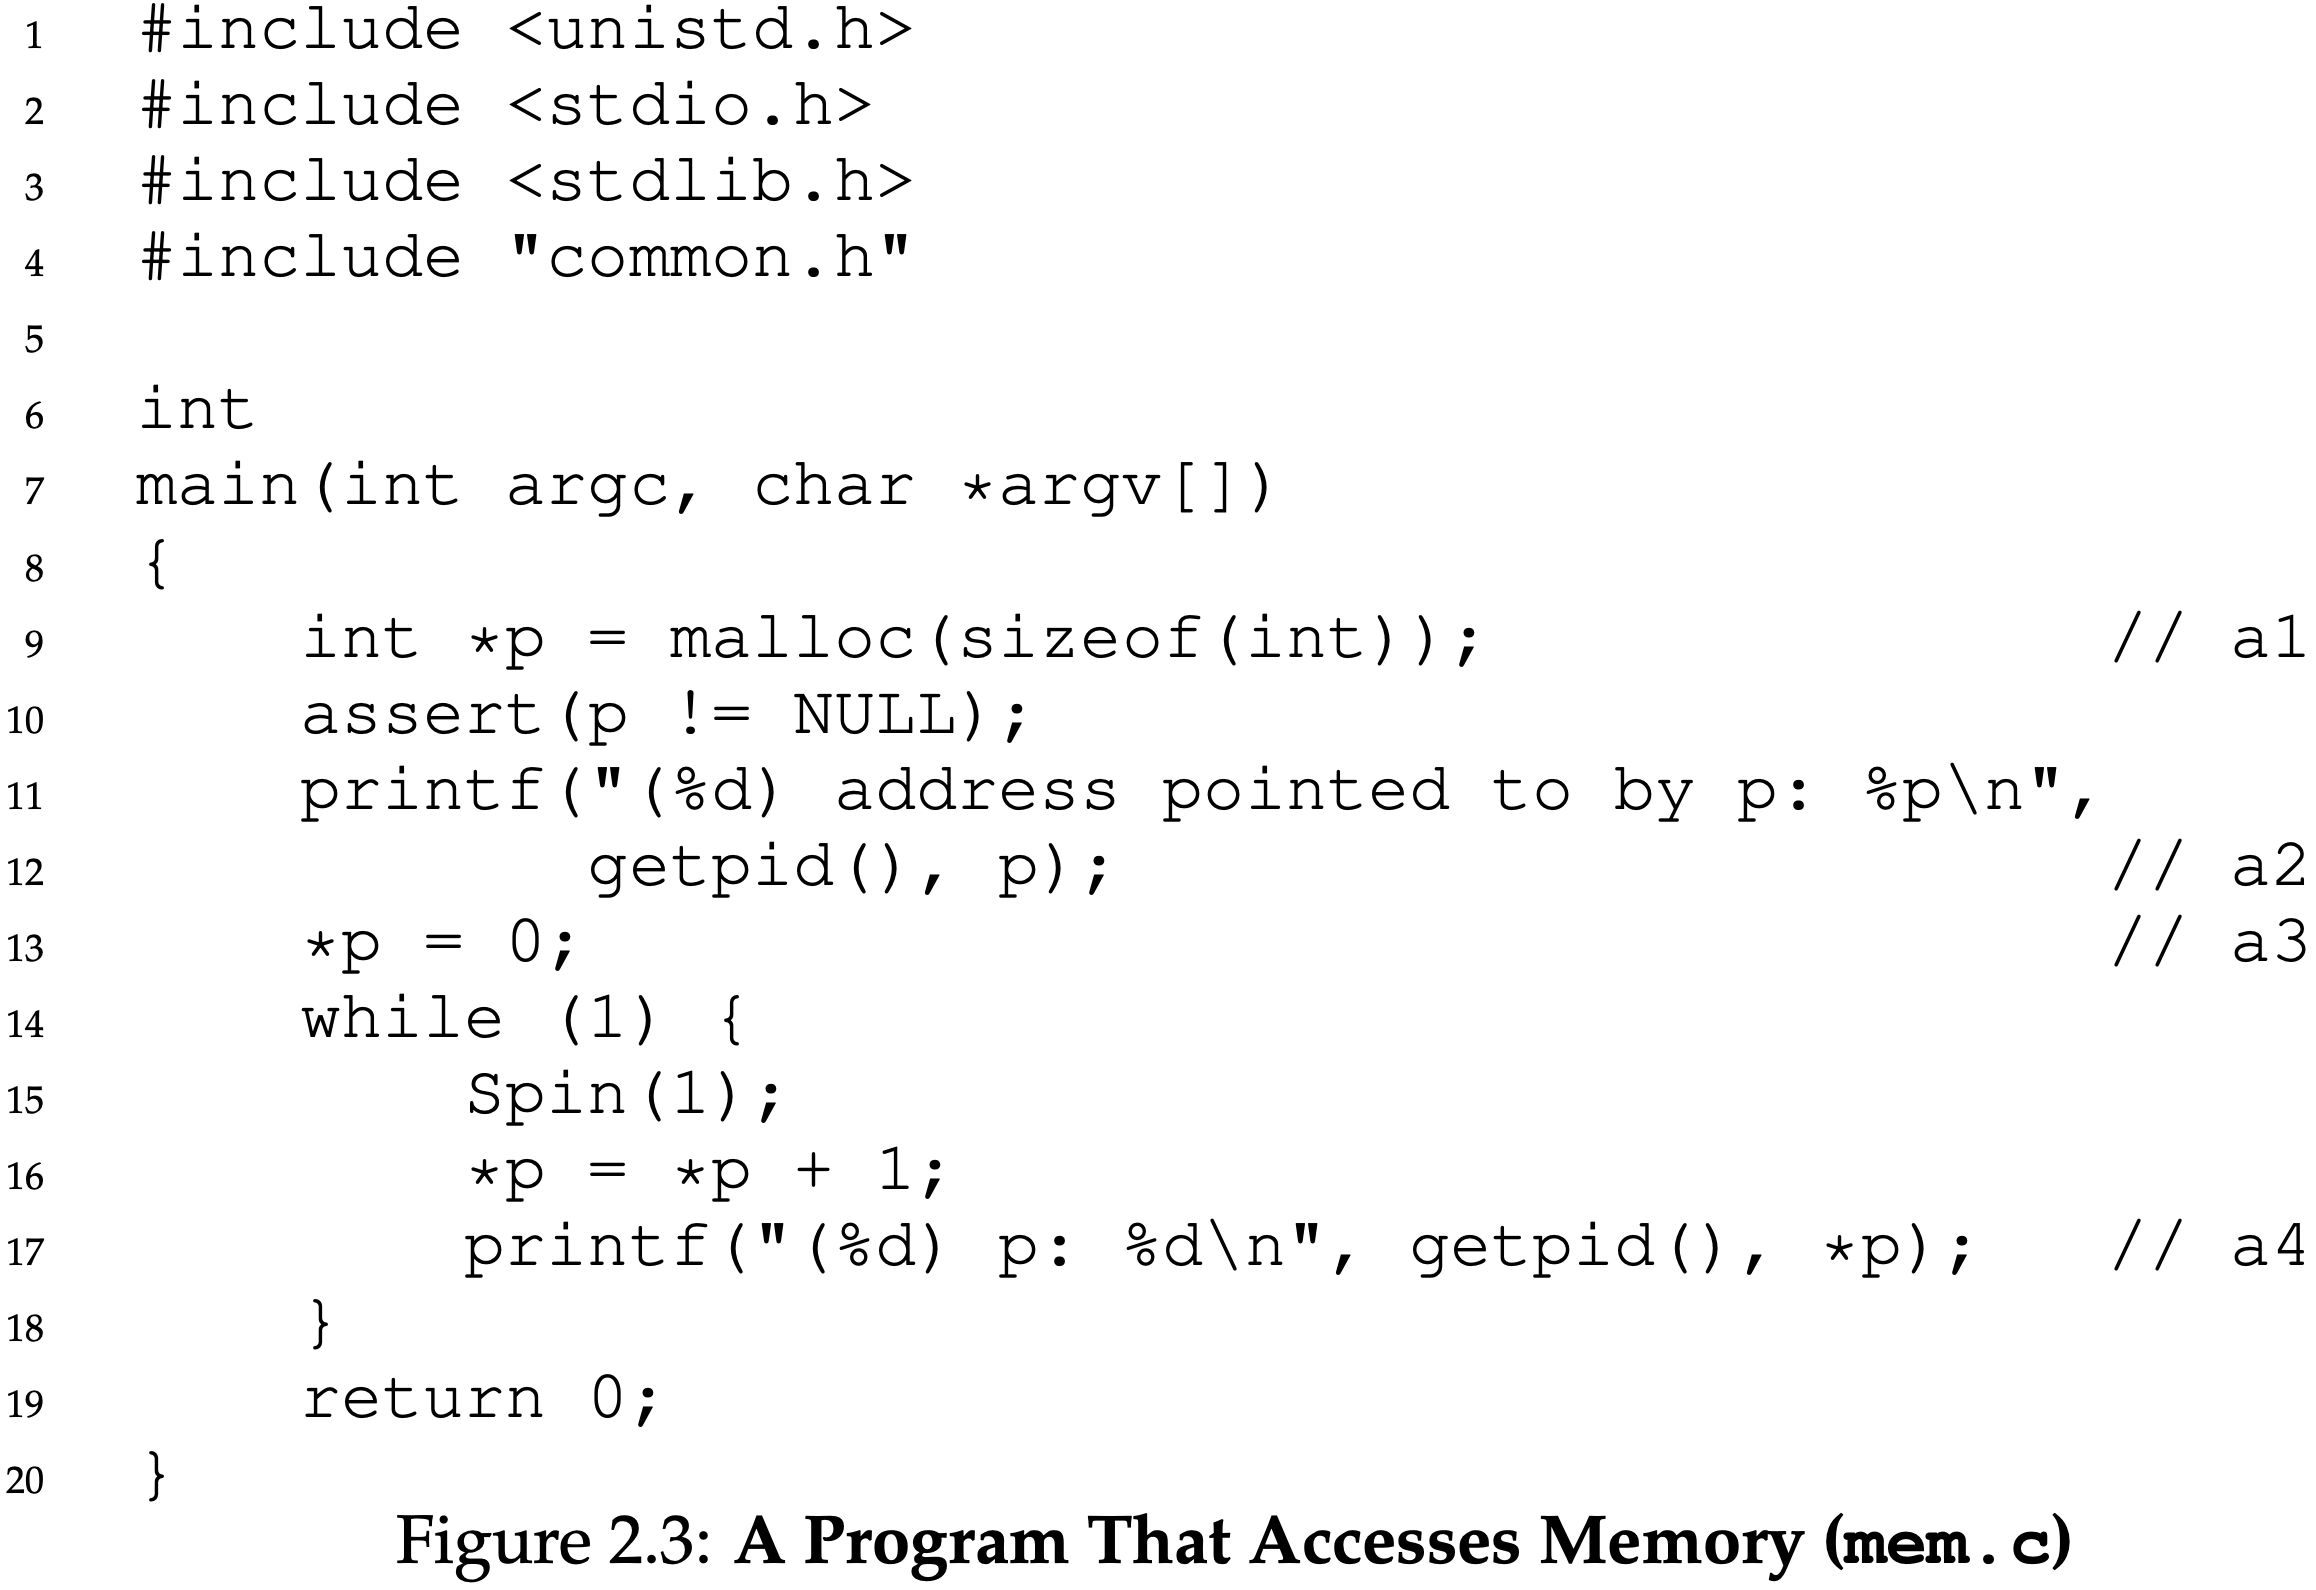
\includegraphics[width=1.1\linewidth]{figs/chapter-2/figure-2.3.png}
        \caption*{Source: chapter page 5.}
        \label{fig:figure-2.3}
    \end{figure}
      % \figureplaceholder{Figure 2.3: mem.c}{Place the book figure here. Source: chapter page 5.}
  \end{columns}
\end{frame}

% Slide 6
\begin{frame}{Private Virtual Address Spaces}
  \begin{columns}[T,onlytextwidth]
    \column{0.48\textwidth}
    \begin{figure}
        \centering
        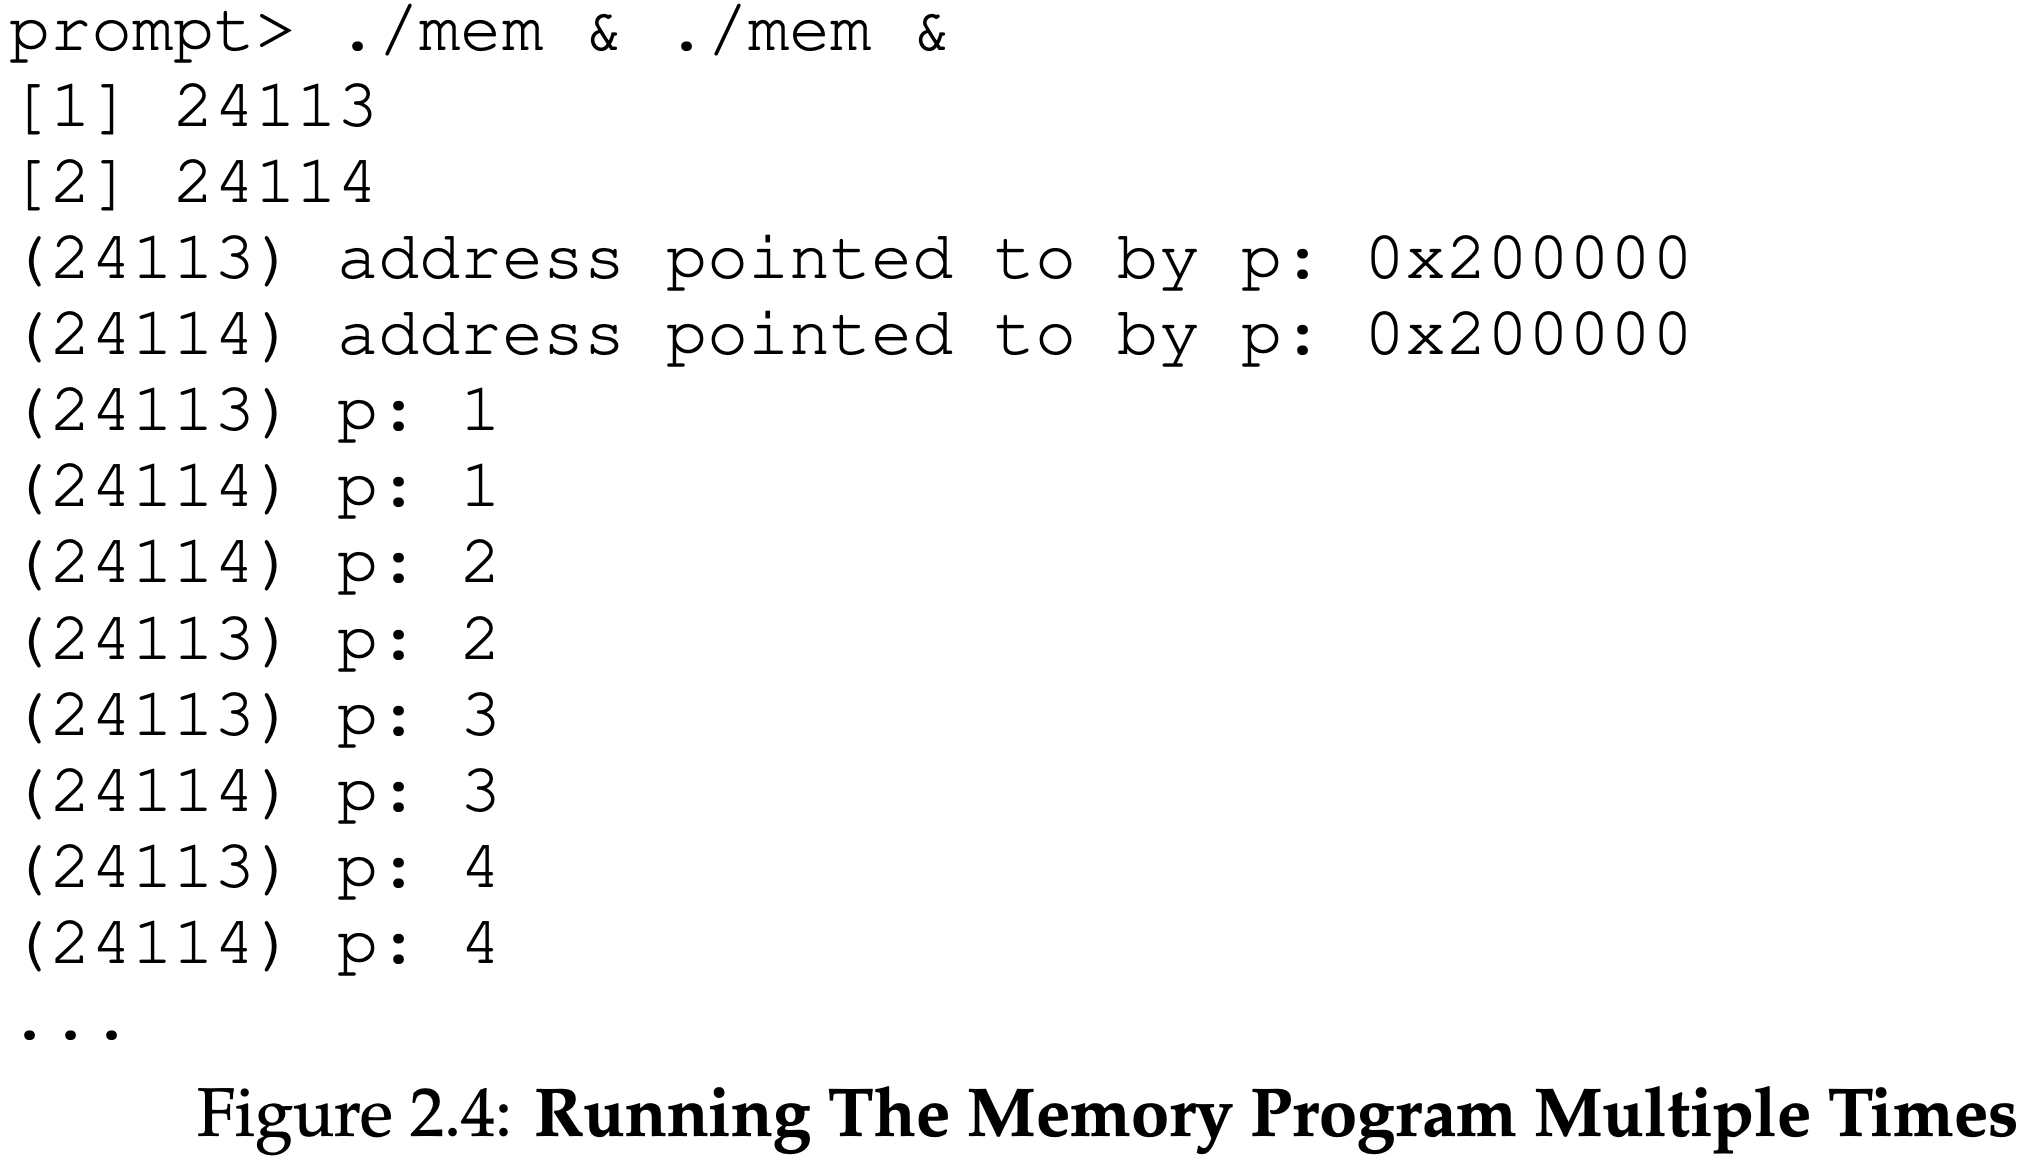
\includegraphics[width=1.1\linewidth]{figs/chapter-2/figure-2.4.png}
        \caption*{Source: chapter page 6.}
        \label{fig:figure-2.4}
    \end{figure}
      % \figureplaceholder{Figure 2.4: Running the Memory Program Multiple Times}{Place the book figure here. Source: chapter page 6.}

    \column{0.50\textwidth}
      \begin{itemize}
        \item Two processes can appear to use the same address independently.
        \item Each process sees its own private \textbf{virtual address space}.
        \item The OS maps each virtual address space onto shared physical memory.
        \item One process normally does not affect another process's address space.
      \end{itemize}
  \end{columns}
\end{frame}

% Slide 7
\begin{frame}{Concurrency}
  \begin{columns}[T,onlytextwidth]
    \column{0.48\textwidth}
      \begin{itemize}
        \item Concurrency refers to problems that arise when multiple activities proceed at the same time.
        \item Modern programs may contain multiple threads sharing the same memory space.
        \item The example creates two worker threads that increment a shared counter.
      \end{itemize}

    \column{0.50\textwidth}
    \begin{figure}
        \centering
        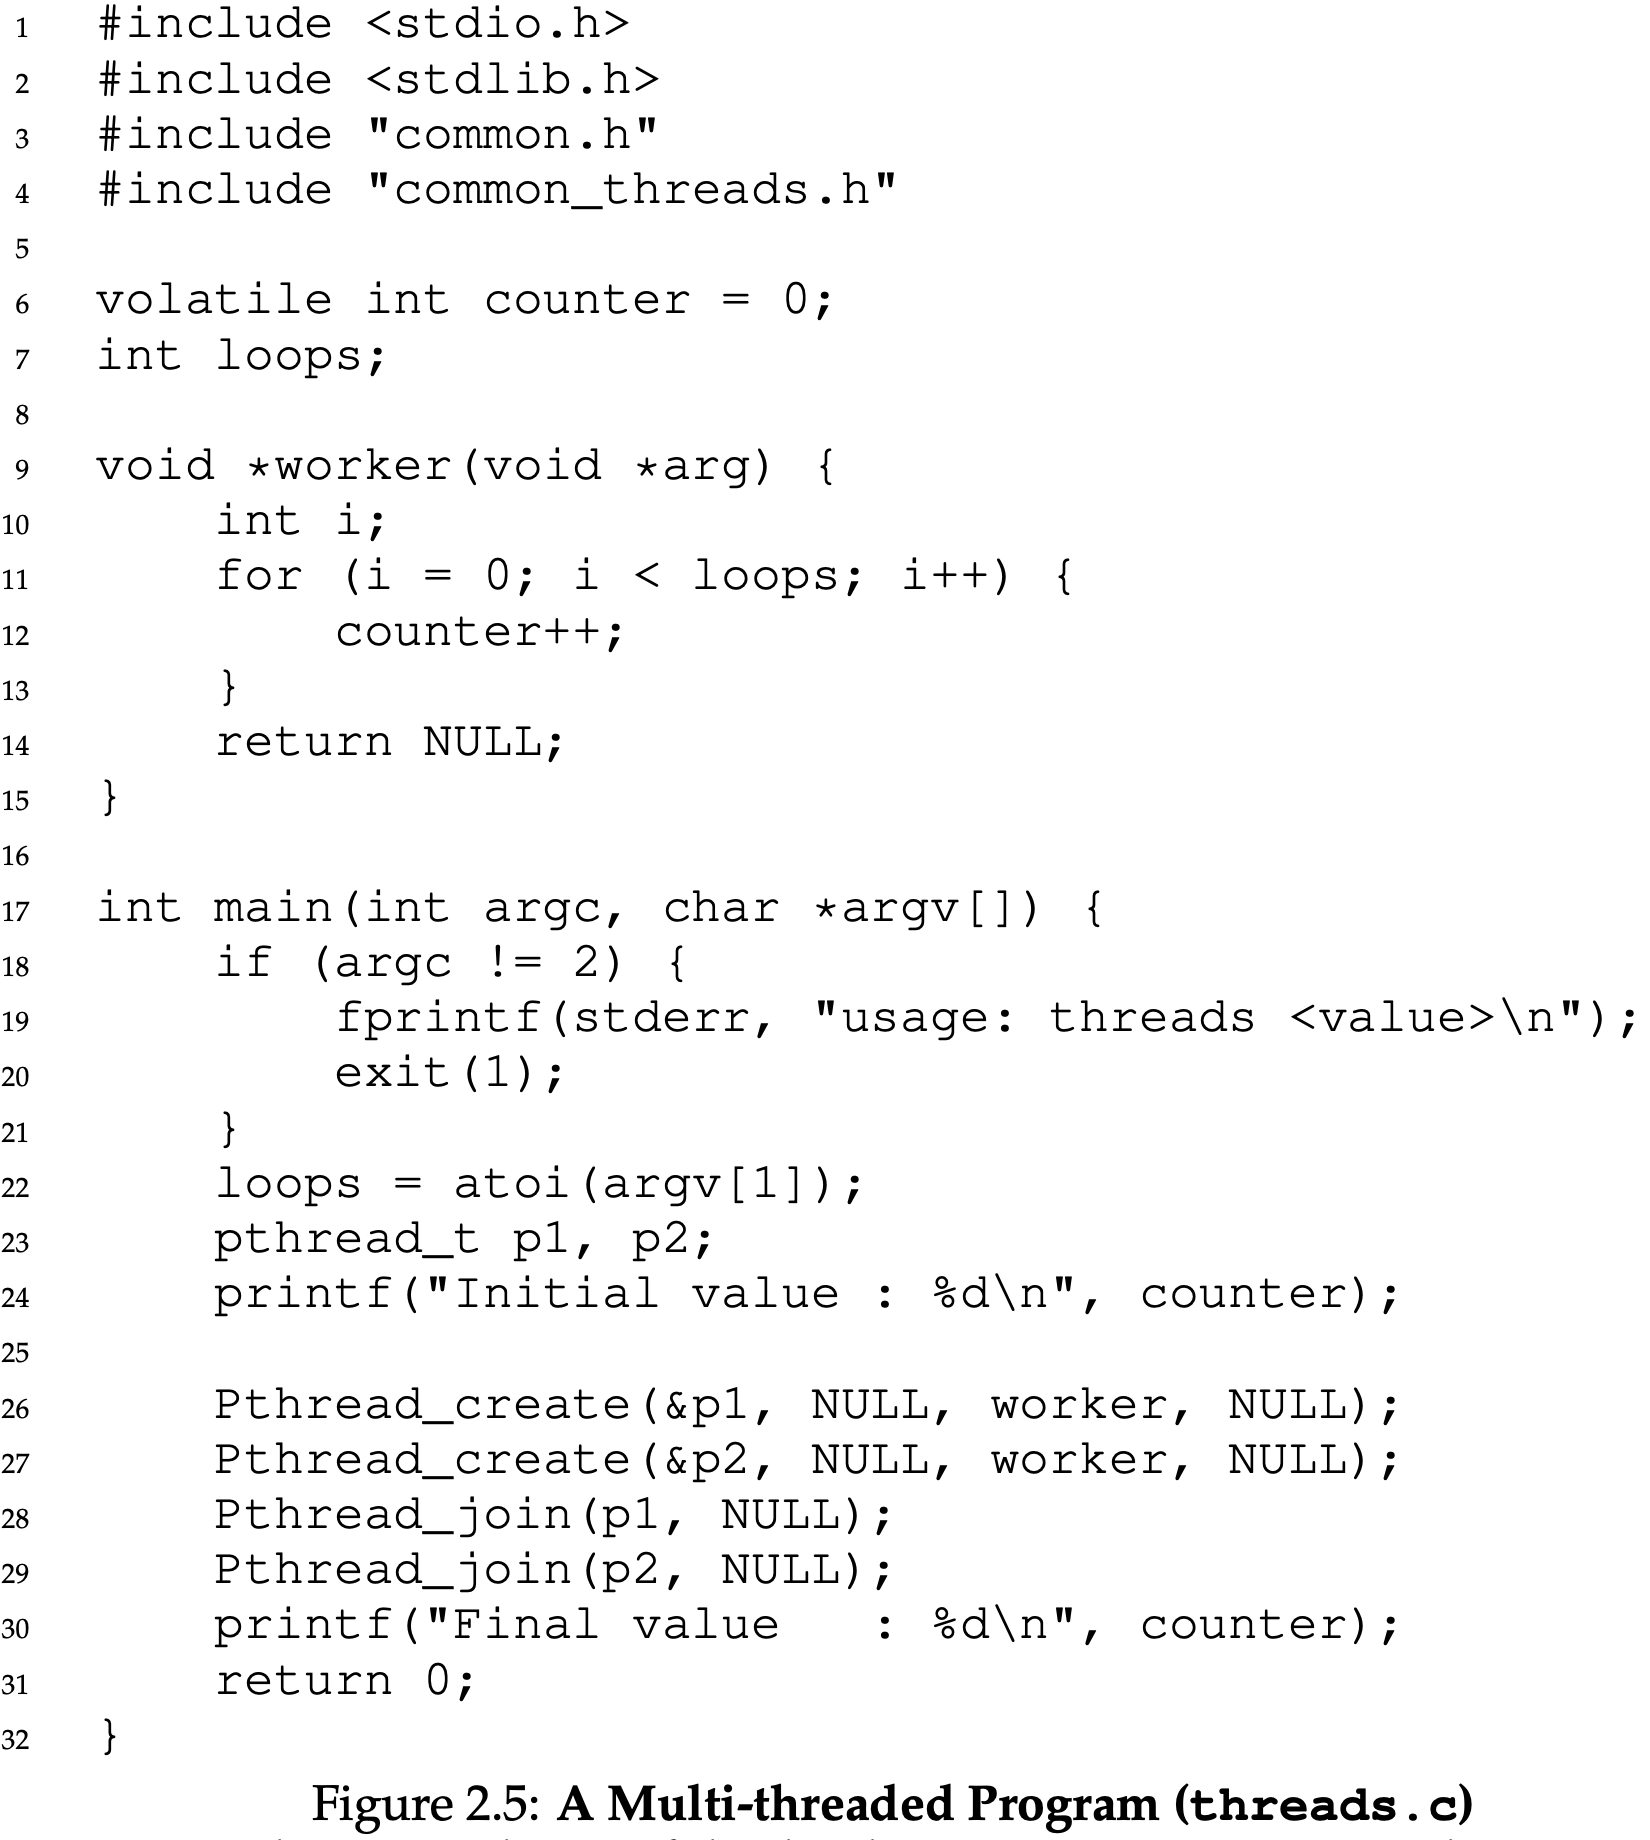
\includegraphics[width=1.1\linewidth]{figs/chapter-2/figure-2.5.png}
        \caption*{Source: chapter page 7.}
        \label{fig:figure-2.5}
    \end{figure}
      % \figureplaceholder{Figure 2.5: threads.c}{Place the book figure here. Source: chapter page 7.}
  \end{columns}
\end{frame}

% Slide 8
\begin{frame}{Why Concurrency Is Difficult}
  \begin{itemize}
    \item With 1,000 increments per thread, the expected final value can be observed.
    \item With larger loop counts, the program may produce incorrect and different results.
    \item Incrementing a shared counter requires multiple machine instructions.
    \item Because the operation is not atomic, thread interleavings can produce unexpected outcomes.
  \end{itemize}

  \vspace{0.5em}
  \begin{alertblock}{The Crux of the Problem}
    How can we build correct programs when many threads execute concurrently in the same memory space?
  \end{alertblock}

  % Source location: shaded ``Crux of the Problem'' box, chapter page 9.
\end{frame}

% Slide 9
\begin{frame}{Persistence}
  \begin{columns}[T,onlytextwidth]
    \column{0.48\textwidth}
      \begin{itemize}
        \item Main memory is volatile: data can disappear after power loss or a crash.
        \item Persistent storage keeps data for the long term.
        \item The file system manages persistent data on storage devices.
        \item Applications use system calls such as \texttt{open()}, \texttt{write()}, and \texttt{close()}.
      \end{itemize}

    \column{0.50\textwidth}
    \begin{figure}
        \centering
        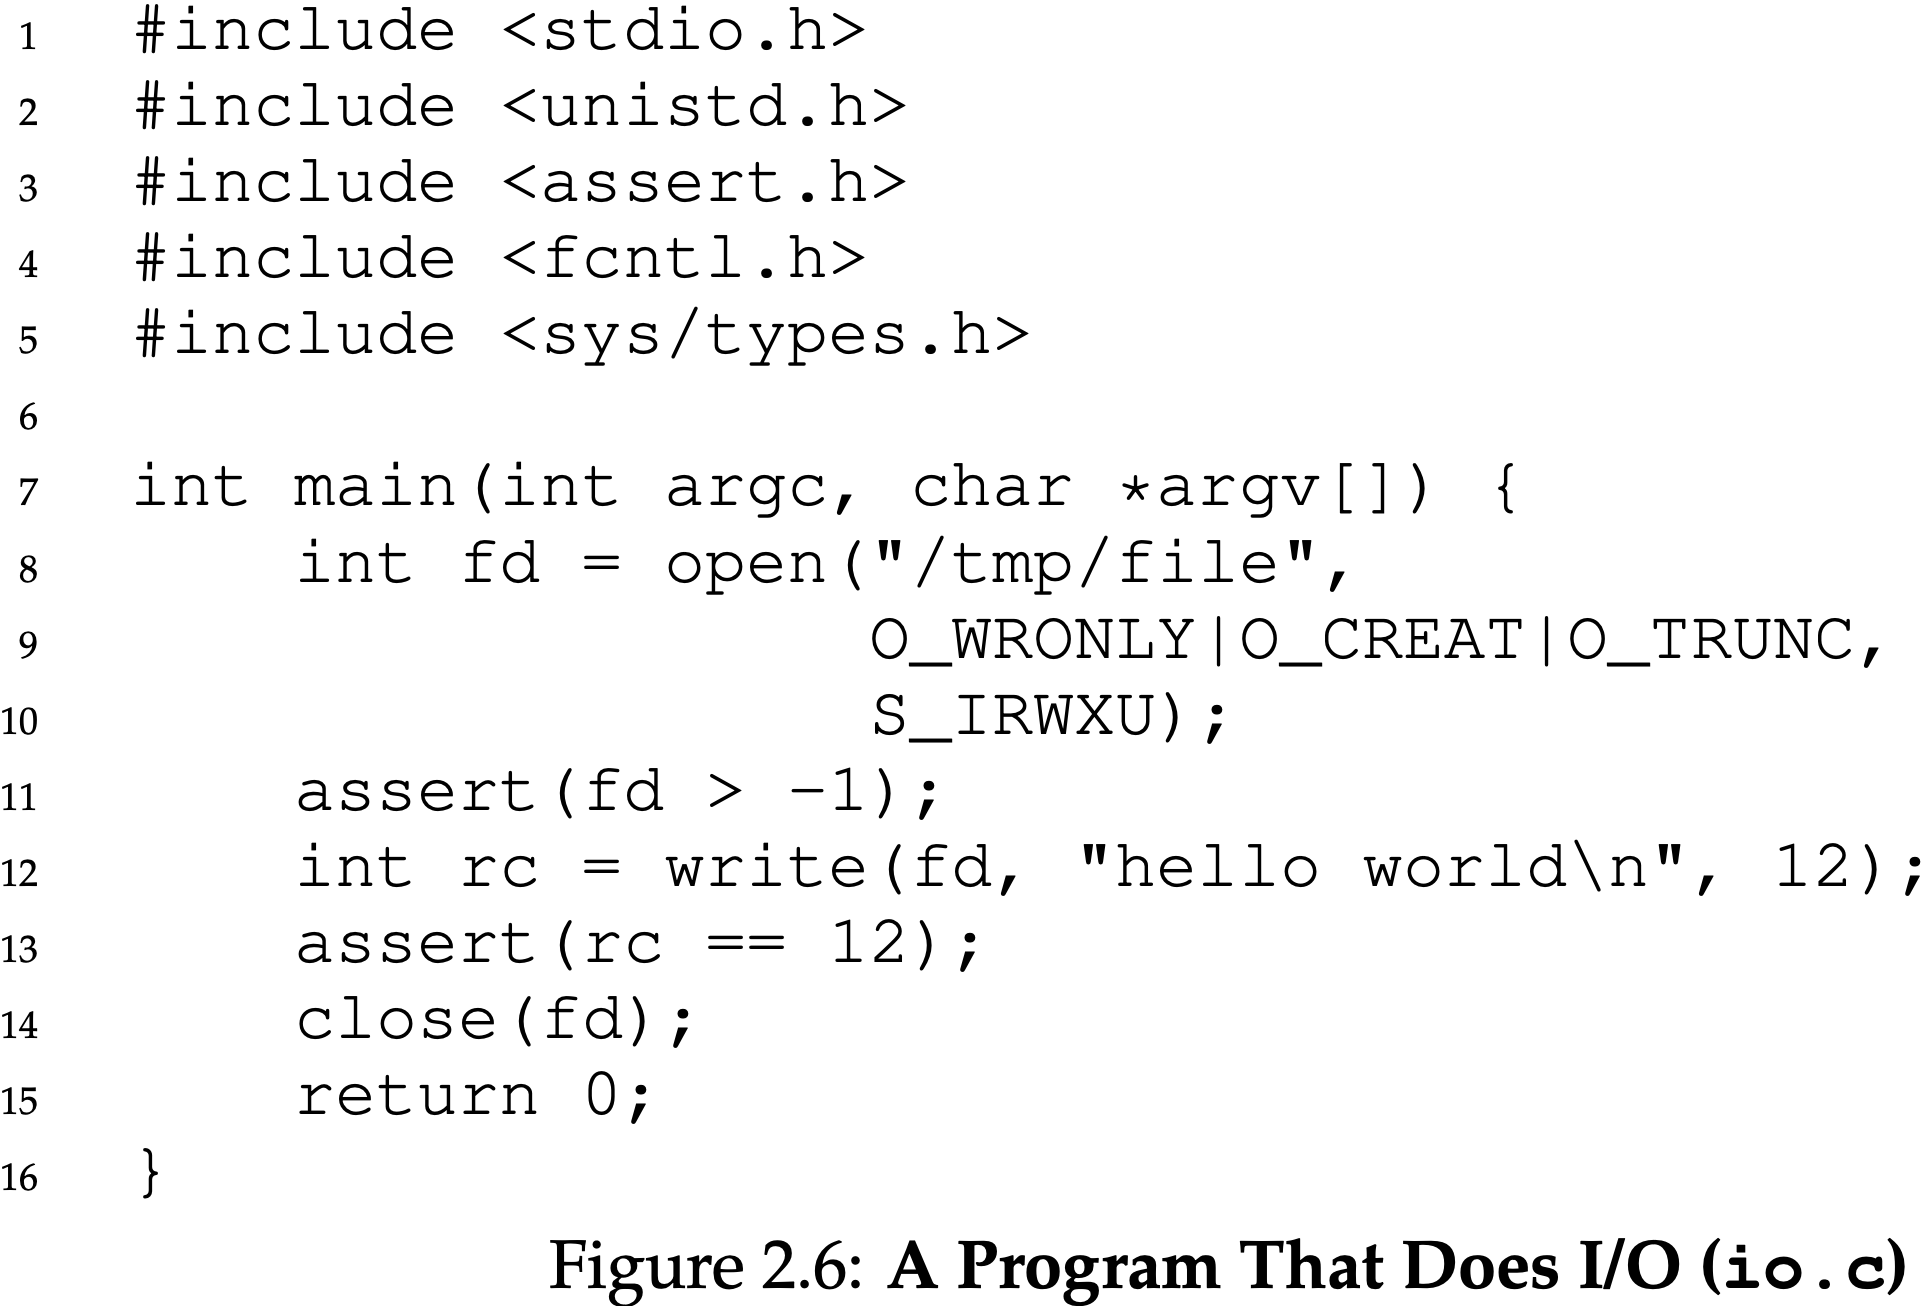
\includegraphics[width=1.1\linewidth]{figs/chapter-2/figure-2.6.png}
        \caption*{Source: chapter page 10.}
        \label{fig:figure-2.6}
    \end{figure}
      % \figureplaceholder{Figure 2.6: io.c}{Place the book figure here. Source: chapter page 10.}
  \end{columns}
\end{frame}

% Slide 10
\begin{frame}{Reliable Persistent Storage}
  \begin{itemize}
    \item File systems must determine where data is stored and maintain metadata about it.
    \item They issue I/O requests to underlying storage devices.
    \item For performance, writes may be delayed and grouped.
    \item Techniques such as \textbf{journaling} and \textbf{copy-on-write} help systems recover from failures.
  \end{itemize}

  \vspace{0.5em}
  \begin{alertblock}{The Crux of the Problem}
    How can the OS store data persistently with correctness, performance, and reliability?
  \end{alertblock}

  % Source location: shaded ``Crux of the Problem'' box, chapter page 11.
\end{frame}

% Slide 11
\begin{frame}{Operating System Design Goals}
  \begin{itemize}
    \item \textbf{Abstraction:} make the system convenient and manageable.
    \item \textbf{Performance:} minimize time and space overheads.
    \item \textbf{Protection and isolation:} prevent applications from harming one another or the OS.
    \item \textbf{Reliability:} keep the operating system running correctly.
    \item Additional goals may include energy efficiency, security, and mobility.
  \end{itemize}
\end{frame}

% Slide 12
\begin{frame}{A Brief History of Operating Systems}
  \begin{enumerate}
    \item \textbf{Early systems:} OS as libraries of common functions; batch processing.
    \item \textbf{Protection:} system calls, user mode, kernel mode, and controlled privilege transitions.
    \item \textbf{Multiprogramming:} several jobs in memory, rapid switching, better CPU utilization.
    \item \textbf{UNIX:} simple, powerful abstractions and tools; strong influence on later systems.
    \item \textbf{Modern era:} mature OS ideas returned to personal computers and later to mobile systems.
  \end{enumerate}

  % Optional visual reference from the chapter:
  % - ``The Importance of UNIX'' aside: chapter page 15.
  % - ``And Then Came Linux'' aside: chapter page 16.
\end{frame}

% Slide 13
\begin{frame}{Chapter Summary}
  \begin{block}{Three Major Themes}
    \begin{enumerate}
      \item \textbf{Virtualization} of the CPU and memory.
      \item \textbf{Concurrency} and correct coordination among simultaneous activities.
      \item \textbf{Persistence} through devices and file systems.
    \end{enumerate}
  \end{block}

  \vspace{0.5em}
  \begin{itemize}
    \item The OS provides abstractions and interfaces that make hardware easier to use.
    \item It manages resources while pursuing performance, protection, and reliability.
  \end{itemize}
\end{frame}

% ---------------------------------------------------------
\begin{frame}{Part I --- Virtualization}

\begin{center}
    \Huge
    \textbf{Virtualization}
\end{center}

\end{frame}

% ---------------------------------------------------------
\section{A Dialogue on Virtualization}

% ---------------------------------------------------------
\begin{frame}{A Dialogue on Virtualization}

{\small
The dialogue introduces \textbf{virtualization} through the metaphor of a
single physical peach being shared among several people, while each person
has the illusion of having their own peach.

\vspace{0.1cm}

The same idea is applied to computing: a physical resource, such as a CPU,
can be shared among multiple applications while each application behaves as
if it had its own dedicated CPU.

\vspace{0.1cm}

The key idea is that the operating system creates this illusion by managing
and sharing physical resources efficiently. In the case of the CPU,
virtualization makes one physical processor appear as multiple virtual CPUs
to running applications.

\vspace{0.1cm}

Thus, virtualization allows several programs to use the same hardware while
giving each one the impression of exclusive access to the resource.
}

\end{frame}
\section{Processes}

% ---------------------------------------------------------
\begin{frame}{The Process Abstraction}

\begin{itemize}
    \item A \textbf{process} is a running program.
    \item A program stored on disk is passive:
    \begin{itemize}
        \item instructions;
        \item static data.
    \end{itemize}
    \item The operating system transforms a program into an active process.
    \item Modern systems execute many processes seemingly at the same time.
\end{itemize}

\begin{alertblock}{Crux of the Problem}
How can the OS provide the illusion of many CPUs when only a few
physical CPUs are available?
\end{alertblock}

\end{frame}

% ---------------------------------------------------------
\begin{frame}{Virtualizing the CPU}

\begin{itemize}
    \item The OS creates the illusion of many virtual CPUs.
    \item It runs one process, stops it, runs another, and so forth.
    \item This technique is called \textbf{time sharing}.
    \item CPU time is shared among concurrent processes.
    \item The main cost of sharing is reduced performance for each process.
\end{itemize}

\vspace{0.3cm}

\begin{block}{Time Sharing}
A resource is used by one entity for a period of time and then
assigned to another.
\end{block}

\end{frame}

% ---------------------------------------------------------
\begin{frame}{Mechanisms and Policies}

\begin{itemize}
    \item CPU virtualization requires two important OS concepts:
\end{itemize}

\begin{block}{Mechanisms}
Low-level methods that implement functionality.

\medskip

Example: stopping one process and starting another through a
\textbf{context switch}.
\end{block}

\begin{block}{Policies}
Algorithms that determine which decision the OS should make.

\medskip

Example: deciding which process should run next.
\end{block}

\begin{center}
\textbf{Mechanism = How? \qquad Policy = Which?}
\end{center}

\end{frame}

% ---------------------------------------------------------
\begin{frame}{What Defines a Process?}

A process can be described through its \textbf{machine state}.

\begin{itemize}
    \item \textbf{Address space}
    \begin{itemize}
        \item program instructions;
        \item program data.
    \end{itemize}

    \item \textbf{CPU registers}
    \begin{itemize}
        \item general-purpose registers;
        \item program counter (PC);
        \item stack pointer;
        \item frame pointer.
    \end{itemize}

    \item \textbf{I/O information}
    \begin{itemize}
        \item open files and other resources.
    \end{itemize}
\end{itemize}

\end{frame}

% ---------------------------------------------------------
\begin{frame}{Process API}

A modern operating system provides interfaces to manage processes.

\begin{itemize}
    \item \textbf{Create}: create a new process.
    \item \textbf{Destroy}: terminate a process.
    \item \textbf{Wait}: wait for a process to finish.
    \item \textbf{Miscellaneous Control}:
          suspend and resume processes.
    \item \textbf{Status}: obtain information about a process.
\end{itemize}

\end{frame}

% ---------------------------------------------------------
\begin{frame}{From Program to Process}

\begin{columns}

\column{0.52\textwidth}

\begin{itemize}
    \item Programs initially reside on persistent storage.
    \item The OS loads:
    \begin{itemize}
        \item program code;
        \item static data.
    \end{itemize}
    \item These elements are placed into the process address space.
    \item The process can then be prepared for execution.
\end{itemize}

\column{0.43\textwidth}
\begin{figure}
    \centering
    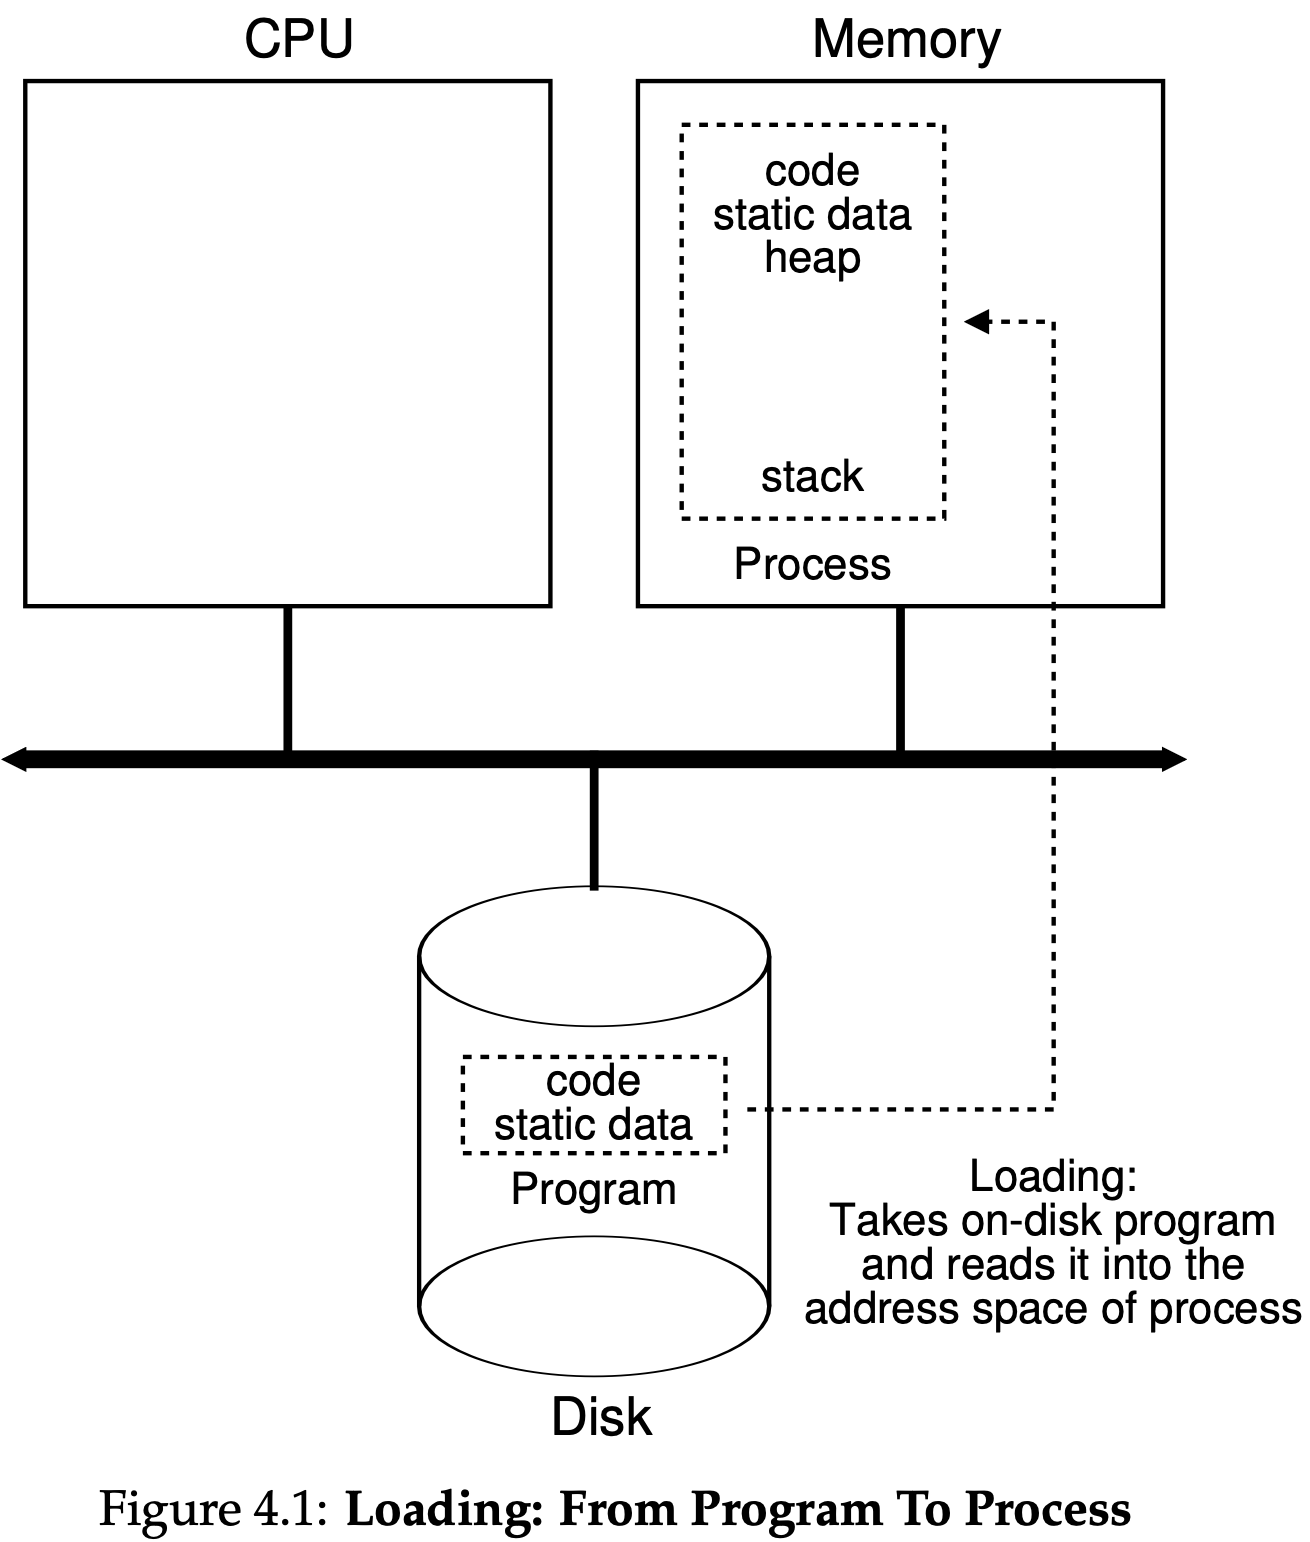
\includegraphics[width=1.1\linewidth]{figs/chapter-4/figure-4.1.png}
    \caption*{Source: chapter page 4.}
    \label{fig:figure-4.1}
\end{figure}
\end{columns}

\end{frame}

% ---------------------------------------------------------
\begin{frame}{Process Creation}

Before starting execution, the OS performs several steps:

\begin{enumerate}
    \item Load code and static data into memory.
    \item Allocate the run-time \textbf{stack}.
    \item Initialize arguments such as \texttt{argc} and \texttt{argv}.
    \item Allocate initial space for the \textbf{heap}.
    \item Initialize I/O resources.
    \item Transfer control to the program entry point.
\end{enumerate}

\vspace{0.2cm}

\begin{block}{UNIX Processes}
A process normally starts with three open file descriptors:
standard input, standard output, and standard error.
\end{block}

\end{frame}

% ---------------------------------------------------------
\begin{frame}{Loading: Eager vs. Lazy}

\begin{itemize}
    \item Early or simple operating systems may load the entire program
          before execution.
\end{itemize}

\begin{block}{Eager Loading}
Code and data are loaded into memory all at once before execution.
\end{block}

\begin{block}{Lazy Loading}
Modern systems can load pieces of code and data only when they
are needed during execution.
\end{block}

\vspace{0.2cm}

Lazy loading is related to memory virtualization mechanisms such as
paging and swapping.

\end{frame}

% ---------------------------------------------------------
\begin{frame}{Process States}

\begin{columns}

\column{0.53\textwidth}

A simplified process model contains three states:

\begin{itemize}
    \item \textbf{Running}: executing instructions on a CPU.
    \item \textbf{Ready}: able to run, but not currently selected.
    \item \textbf{Blocked}: waiting for an event, such as I/O completion.
\end{itemize}

\column{0.42\textwidth}
\begin{figure}
    \centering
    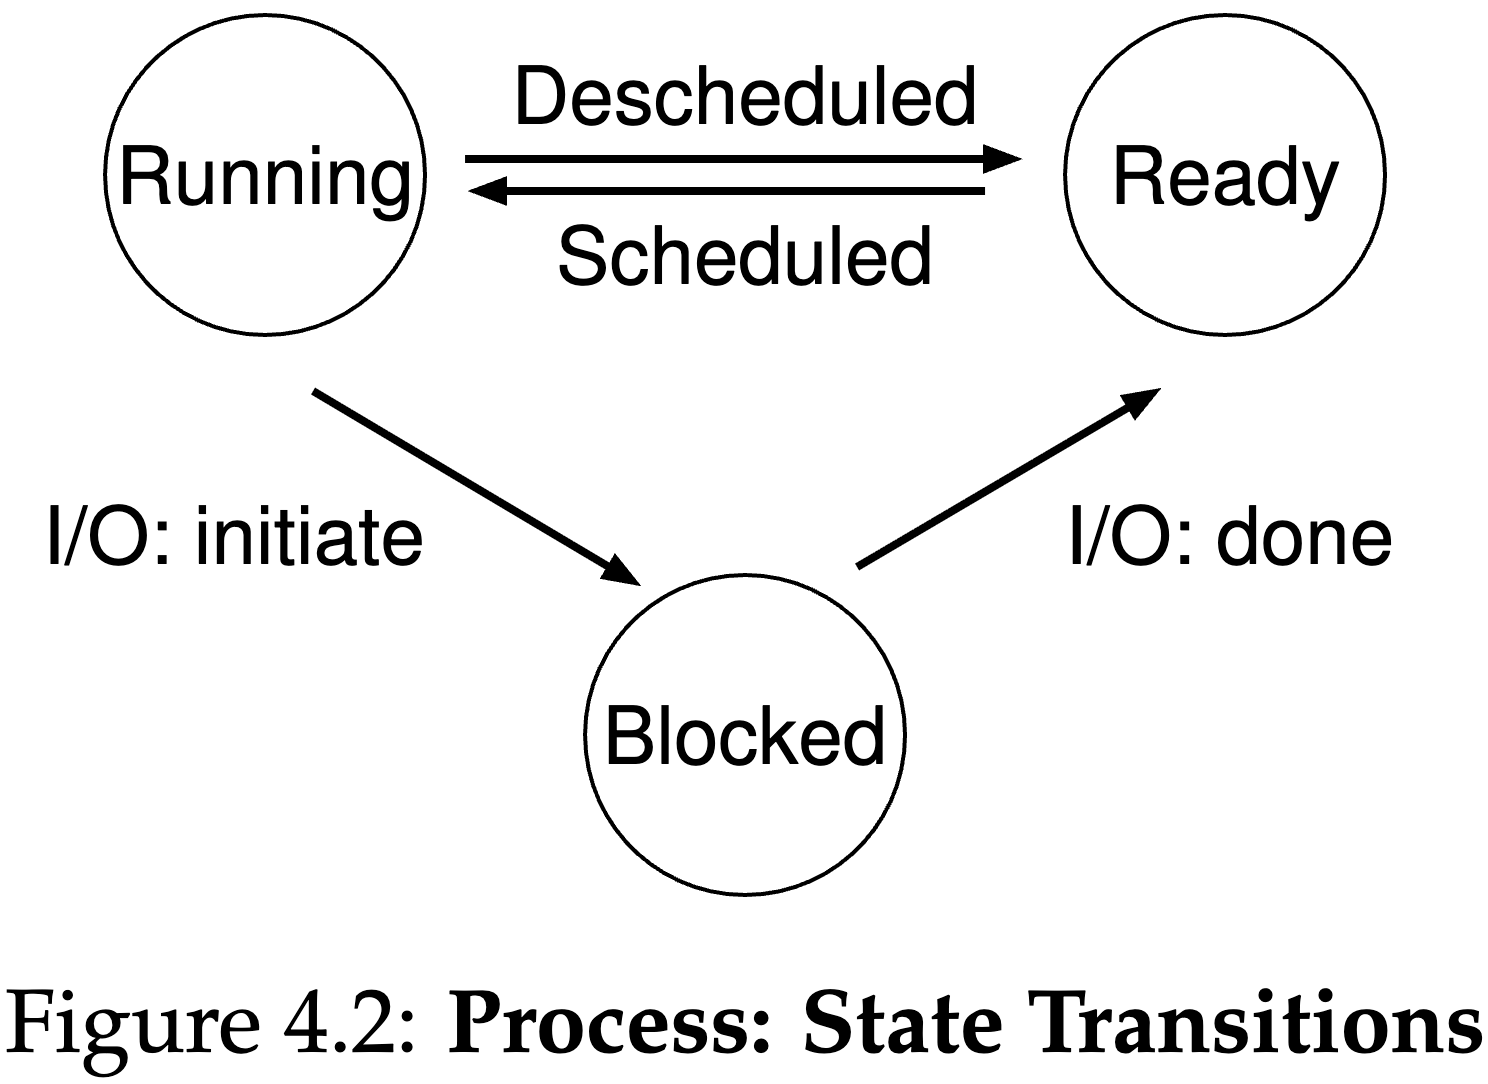
\includegraphics[width=1.1\linewidth]{figs/chapter-4/figure-4.2.png}
    \caption*{Source: chapter page 6}
    \label{fig:figure-4.2}
\end{figure}
\end{columns}

\end{frame}

% ---------------------------------------------------------
\begin{frame}{Process State Transitions}

\begin{itemize}
    \item \textbf{Ready $\rightarrow$ Running}
    \begin{itemize}
        \item the process is \textbf{scheduled}.
    \end{itemize}

    \item \textbf{Running $\rightarrow$ Ready}
    \begin{itemize}
        \item the process is \textbf{descheduled}.
    \end{itemize}

    \item \textbf{Running $\rightarrow$ Blocked}
    \begin{itemize}
        \item the process initiates an operation such as I/O.
    \end{itemize}

    \item \textbf{Blocked $\rightarrow$ Ready}
    \begin{itemize}
        \item the event or I/O operation completes.
    \end{itemize}
\end{itemize}

\end{frame}

% ---------------------------------------------------------
\begin{frame}{Example: CPU-Only Processes}

\begin{columns}

\column{0.48\textwidth}

\begin{itemize}
    \item Consider two processes that only use the CPU.
    \item One process runs while the other remains ready.
    \item When the first process finishes, the second can run.
\end{itemize}

\column{0.47\textwidth}
\begin{figure}
    \centering
    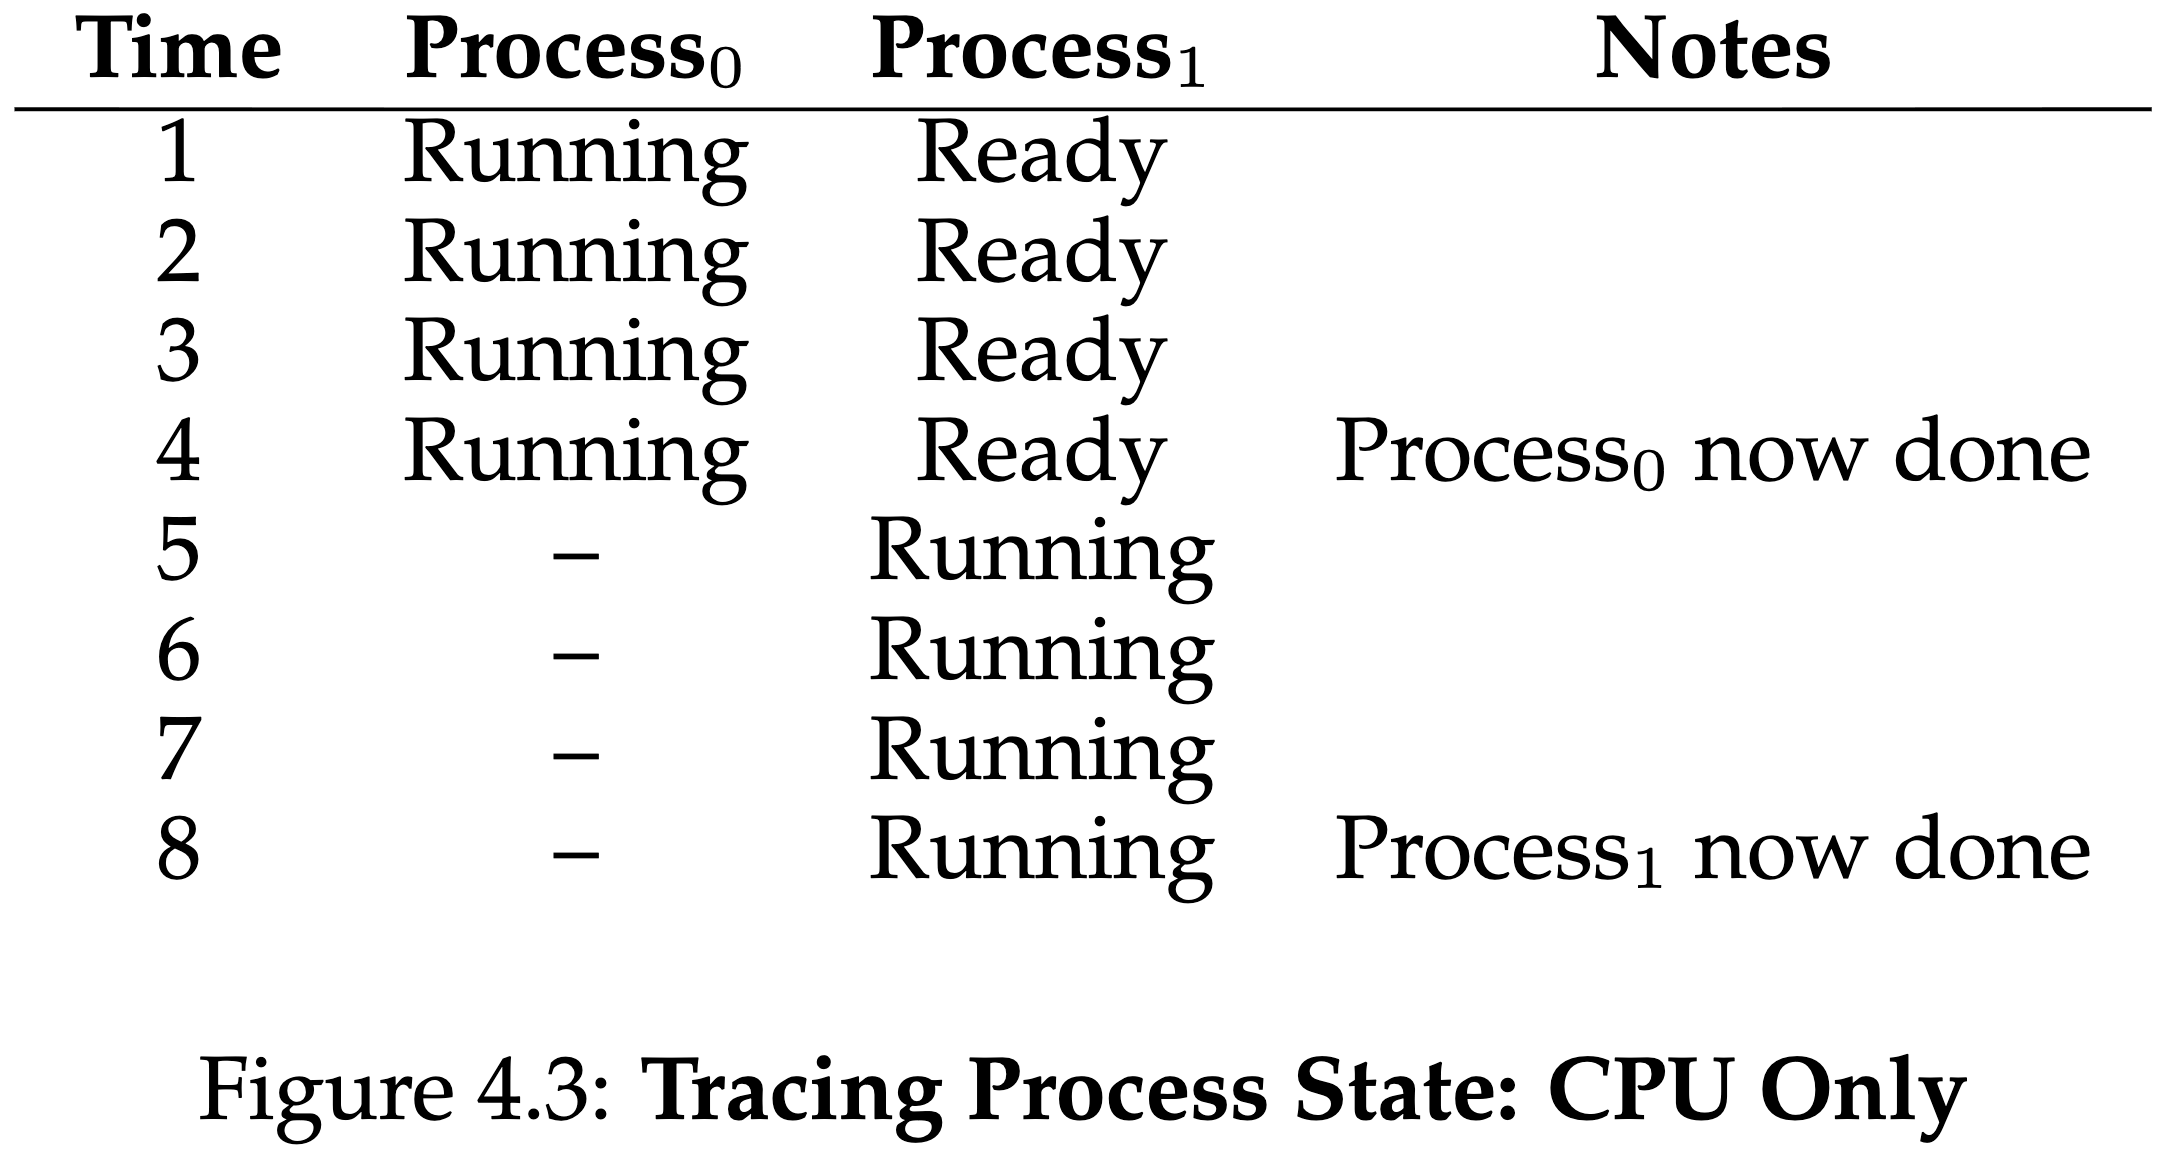
\includegraphics[width=1.1\linewidth]{figs/chapter-4/figure-4.3.png}
    \caption*{Source: chapter page 6.}
    \label{fig:figure-4.3}
\end{figure}
\end{columns}

\end{frame}

% ---------------------------------------------------------
\begin{frame}{Example: CPU and I/O}

\begin{columns}

\column{0.50\textwidth}

\begin{itemize}
    \item Process0 starts running.
    \item Process0 initiates I/O and becomes blocked.
    \item Process1 uses the CPU while Process0 waits.
    \item When I/O completes, Process0 becomes ready again.
    \item This improves CPU utilization.
\end{itemize}

\column{0.45\textwidth}
\begin{figure}
    \centering
    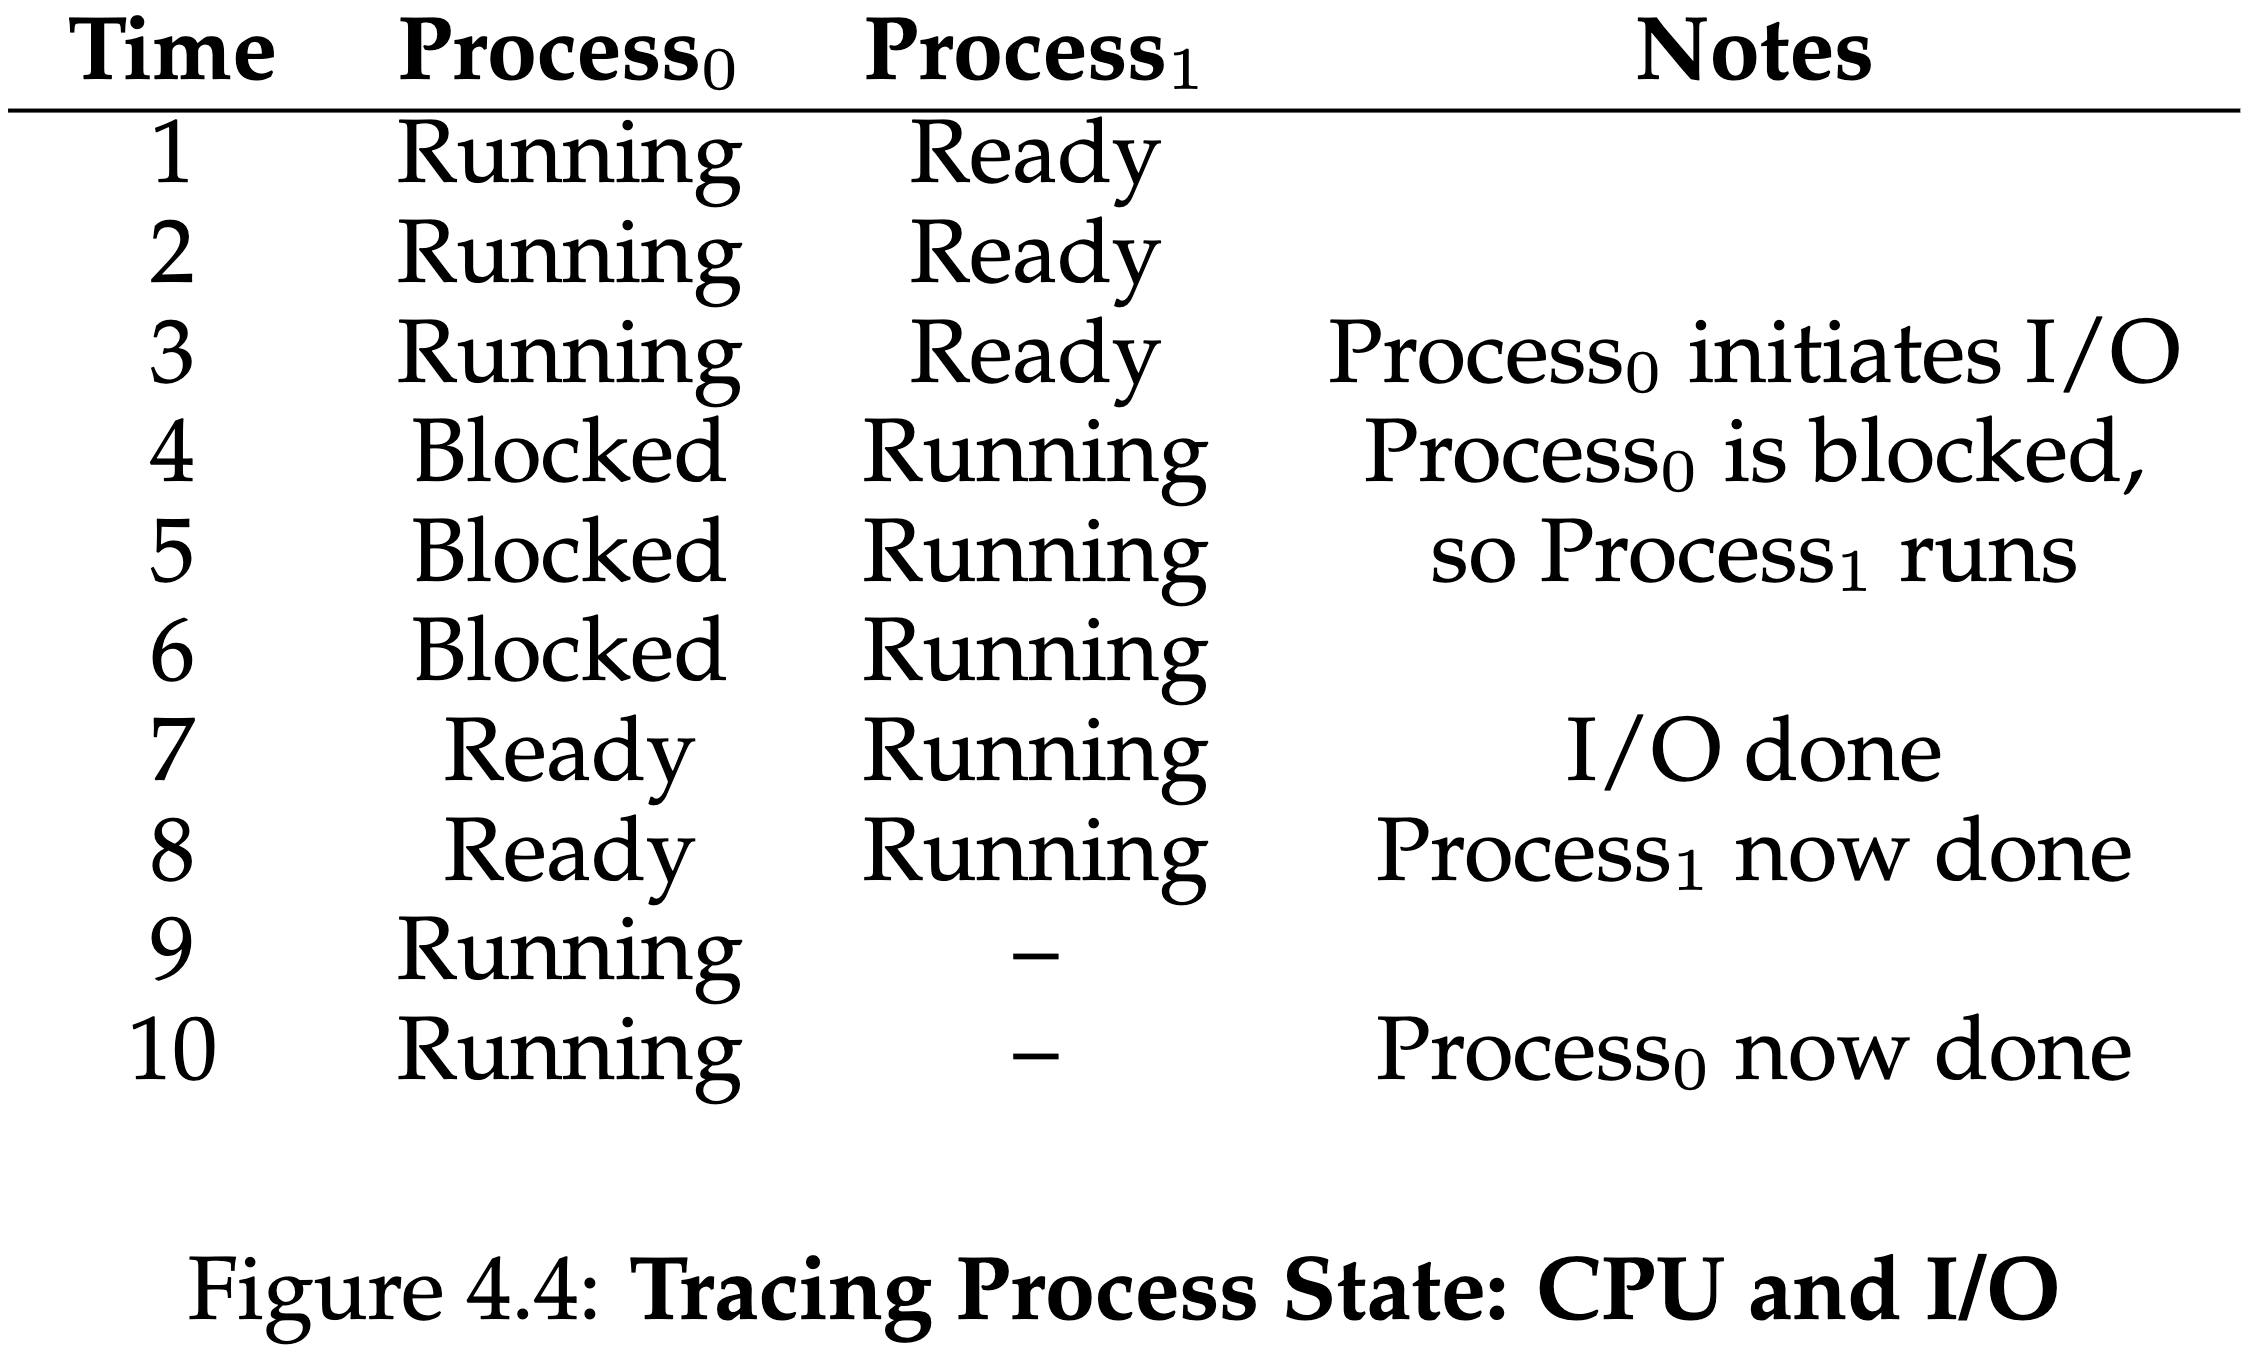
\includegraphics[width=1.1\linewidth]{figs/chapter-4/figure-4.4.png}
    \caption*{Source: chapter page 7.}
    \label{fig:figure-4.4}
\end{figure}
\end{columns}

\end{frame}

% ---------------------------------------------------------
\begin{frame}{Scheduling Decisions}

Even a simple CPU/I/O example requires OS decisions.

\begin{itemize}
    \item Which ready process should run?
    \item Should the OS switch processes when one becomes blocked?
    \item Should a process run immediately after its I/O completes?
    \item Should the currently running process continue?
\end{itemize}

\vspace{0.3cm}

\begin{block}{Scheduler}
The OS component responsible for deciding which process should
use the CPU.
\end{block}

\end{frame}

% ---------------------------------------------------------
\begin{frame}{Process Data Structures}

\begin{columns}

\column{0.48\textwidth}

The OS must keep information about every process.

\begin{itemize}
    \item process state;
    \item process identifier (PID);
    \item memory information;
    \item register context;
    \item open files;
    \item parent process;
    \item current directory.
\end{itemize}

\column{0.47\textwidth}
\begin{figure}
    \centering
    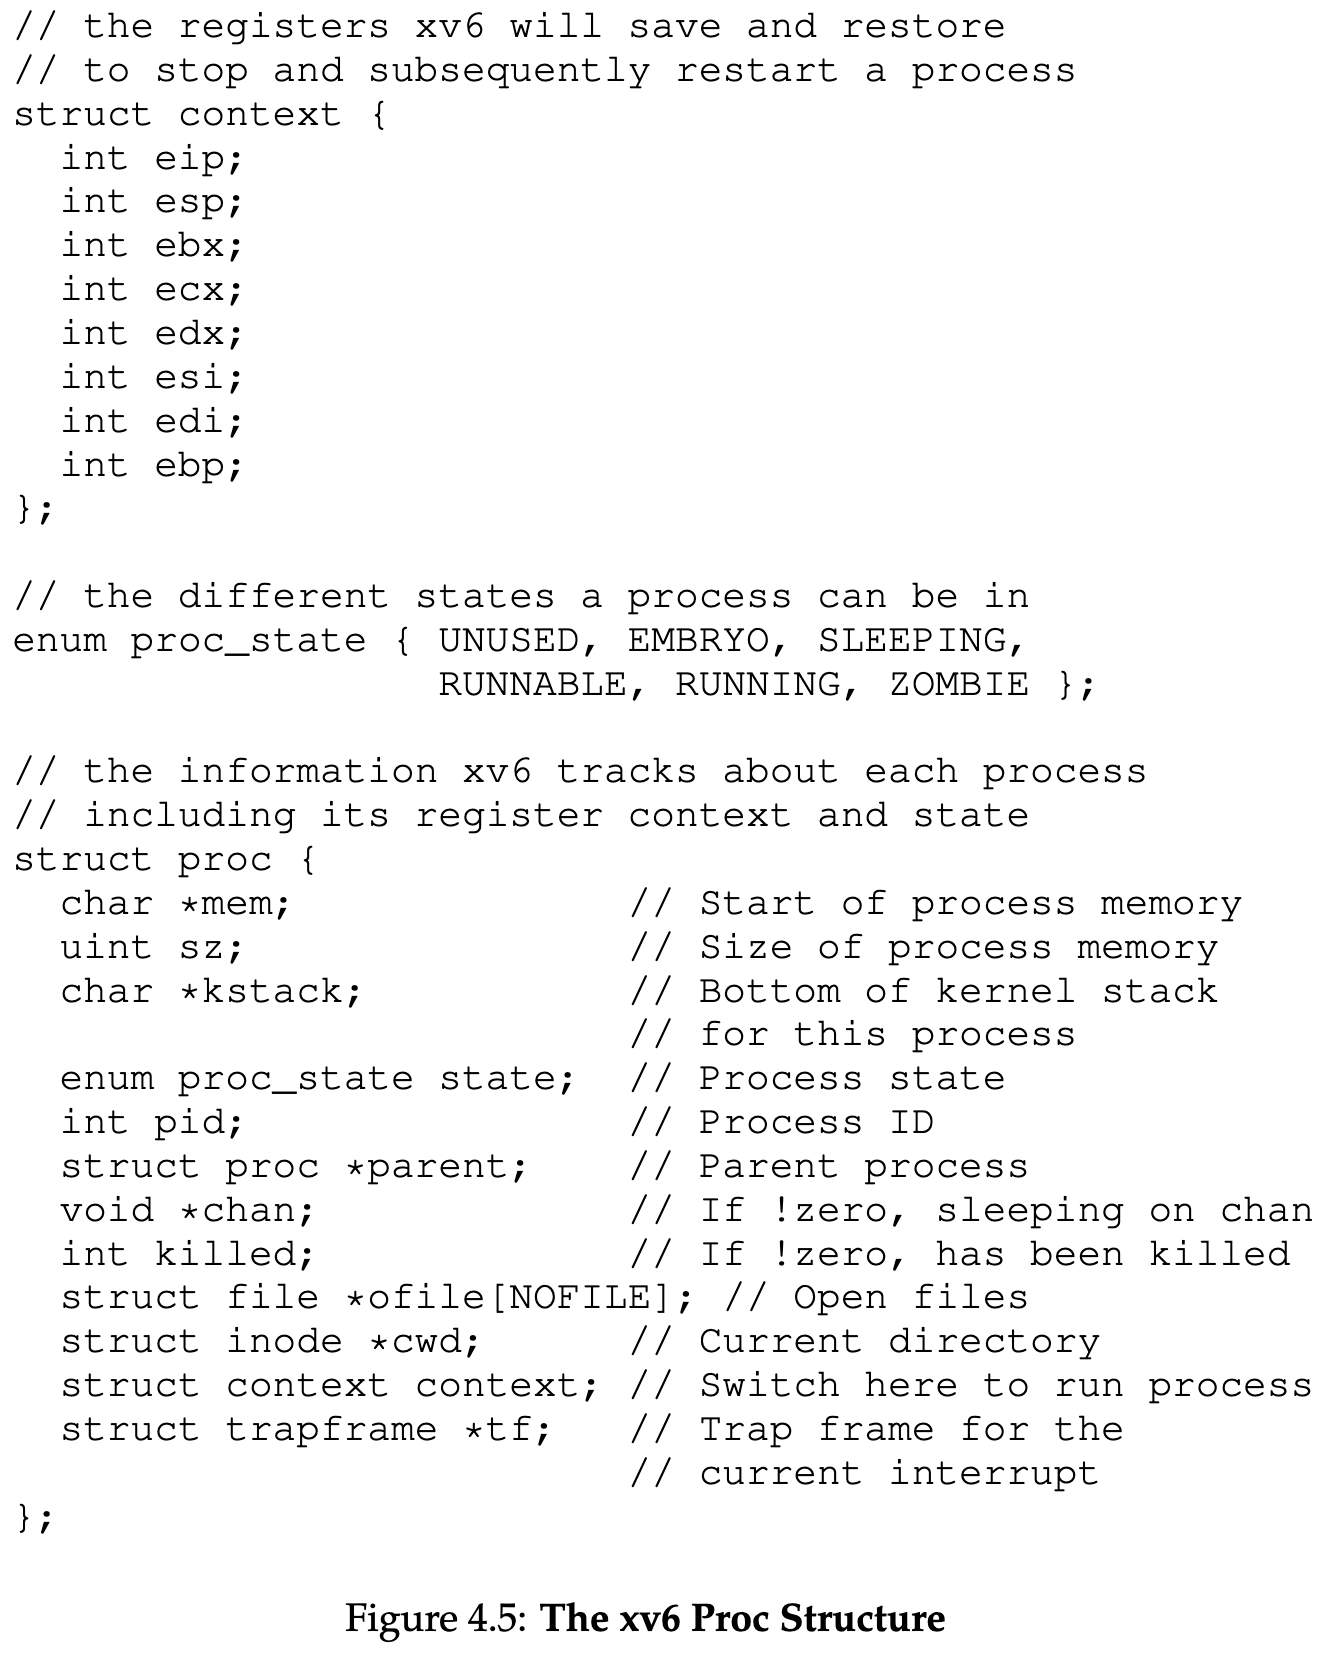
\includegraphics[width=1.1\linewidth]{figs/chapter-4/figure-4.5.png}
    \caption*{Source: chapter page 8.}
    \label{fig:figure-4.5}
\end{figure}
\end{columns}

\end{frame}

% ---------------------------------------------------------
\begin{frame}{Process List and PCB}

\begin{itemize}
    \item The OS maintains a \textbf{process list} or \textbf{task list}.
    \item It tracks:
    \begin{itemize}
        \item ready processes;
        \item running processes;
        \item blocked processes.
    \end{itemize}
    \item Information about an individual process is often stored in a
          \textbf{Process Control Block (PCB)}.
    \item The saved register context allows the OS to stop and later
          resume a process.
\end{itemize}

\begin{block}{Context Switch}
The OS saves the state of one process and restores the state
of another process.
\end{block}

\end{frame}

% ---------------------------------------------------------
\begin{frame}{Additional Process States}

Real operating systems may use more states than the simplified model.

\begin{itemize}
    \item A process may have an initial state while it is being created.
    \item A process may remain temporarily after it finishes execution.
\end{itemize}

\begin{block}{Zombie State}
In UNIX-based systems, an exited process can remain in a zombie
state until its parent obtains its return status, typically using
\texttt{wait()}.
\end{block}

\end{frame}

% ---------------------------------------------------------
\begin{frame}{Chapter Summary}

\begin{itemize}
    \item A \textbf{process} is the OS abstraction of a running program.
    \item CPU virtualization allows many processes to share a small
          number of physical CPUs.
    \item A process is characterized by:
    \begin{itemize}
        \item its address space;
        \item CPU registers;
        \item I/O state.
    \end{itemize}
    \item Processes transition among states such as
          \textbf{running}, \textbf{ready}, and \textbf{blocked}.
    \item The OS tracks processes through structures such as the
          \textbf{process list} and \textbf{PCB}.
    \item Mechanisms and policies together enable CPU virtualization.
\end{itemize}

\end{frame}
% =========================================================
% Section: Process API
% =========================================================

\section{Process API}

% ---------------------------------------------------------
\begin{frame}{Process Creation and Control}

\begin{block}{Key Question}
What interfaces should the operating system provide for
\textbf{process creation and control}?
\end{block}

\begin{itemize}
    \item UNIX provides a distinctive process creation API.
    \item Three fundamental system calls:
    \begin{itemize}
        \item \texttt{fork()} -- create a new process;
        \item \texttt{exec()} -- execute a different program;
        \item \texttt{wait()} -- wait for a child process to finish.
    \end{itemize}
\end{itemize}

\end{frame}

% ---------------------------------------------------------
\begin{frame}{The \texttt{fork()} System Call}

\begin{columns}[T]

\begin{column}{0.47\textwidth}
\begin{itemize}
    \item \texttt{fork()} creates a new process.
    \item The original process is the \textbf{parent}.
    \item The newly created process is the \textbf{child}.
    \item The child is an almost exact copy of the parent.
    \item Both continue execution after \texttt{fork()}.
\end{itemize}

\begin{block}{Return Value}
\begin{itemize}
    \item Parent: child PID.
    \item Child: \texttt{0}.
    \item Failure: negative value.
\end{itemize}
\end{block}
\end{column}

\begin{column}{0.50\textwidth}
\begin{figure}
    \centering
    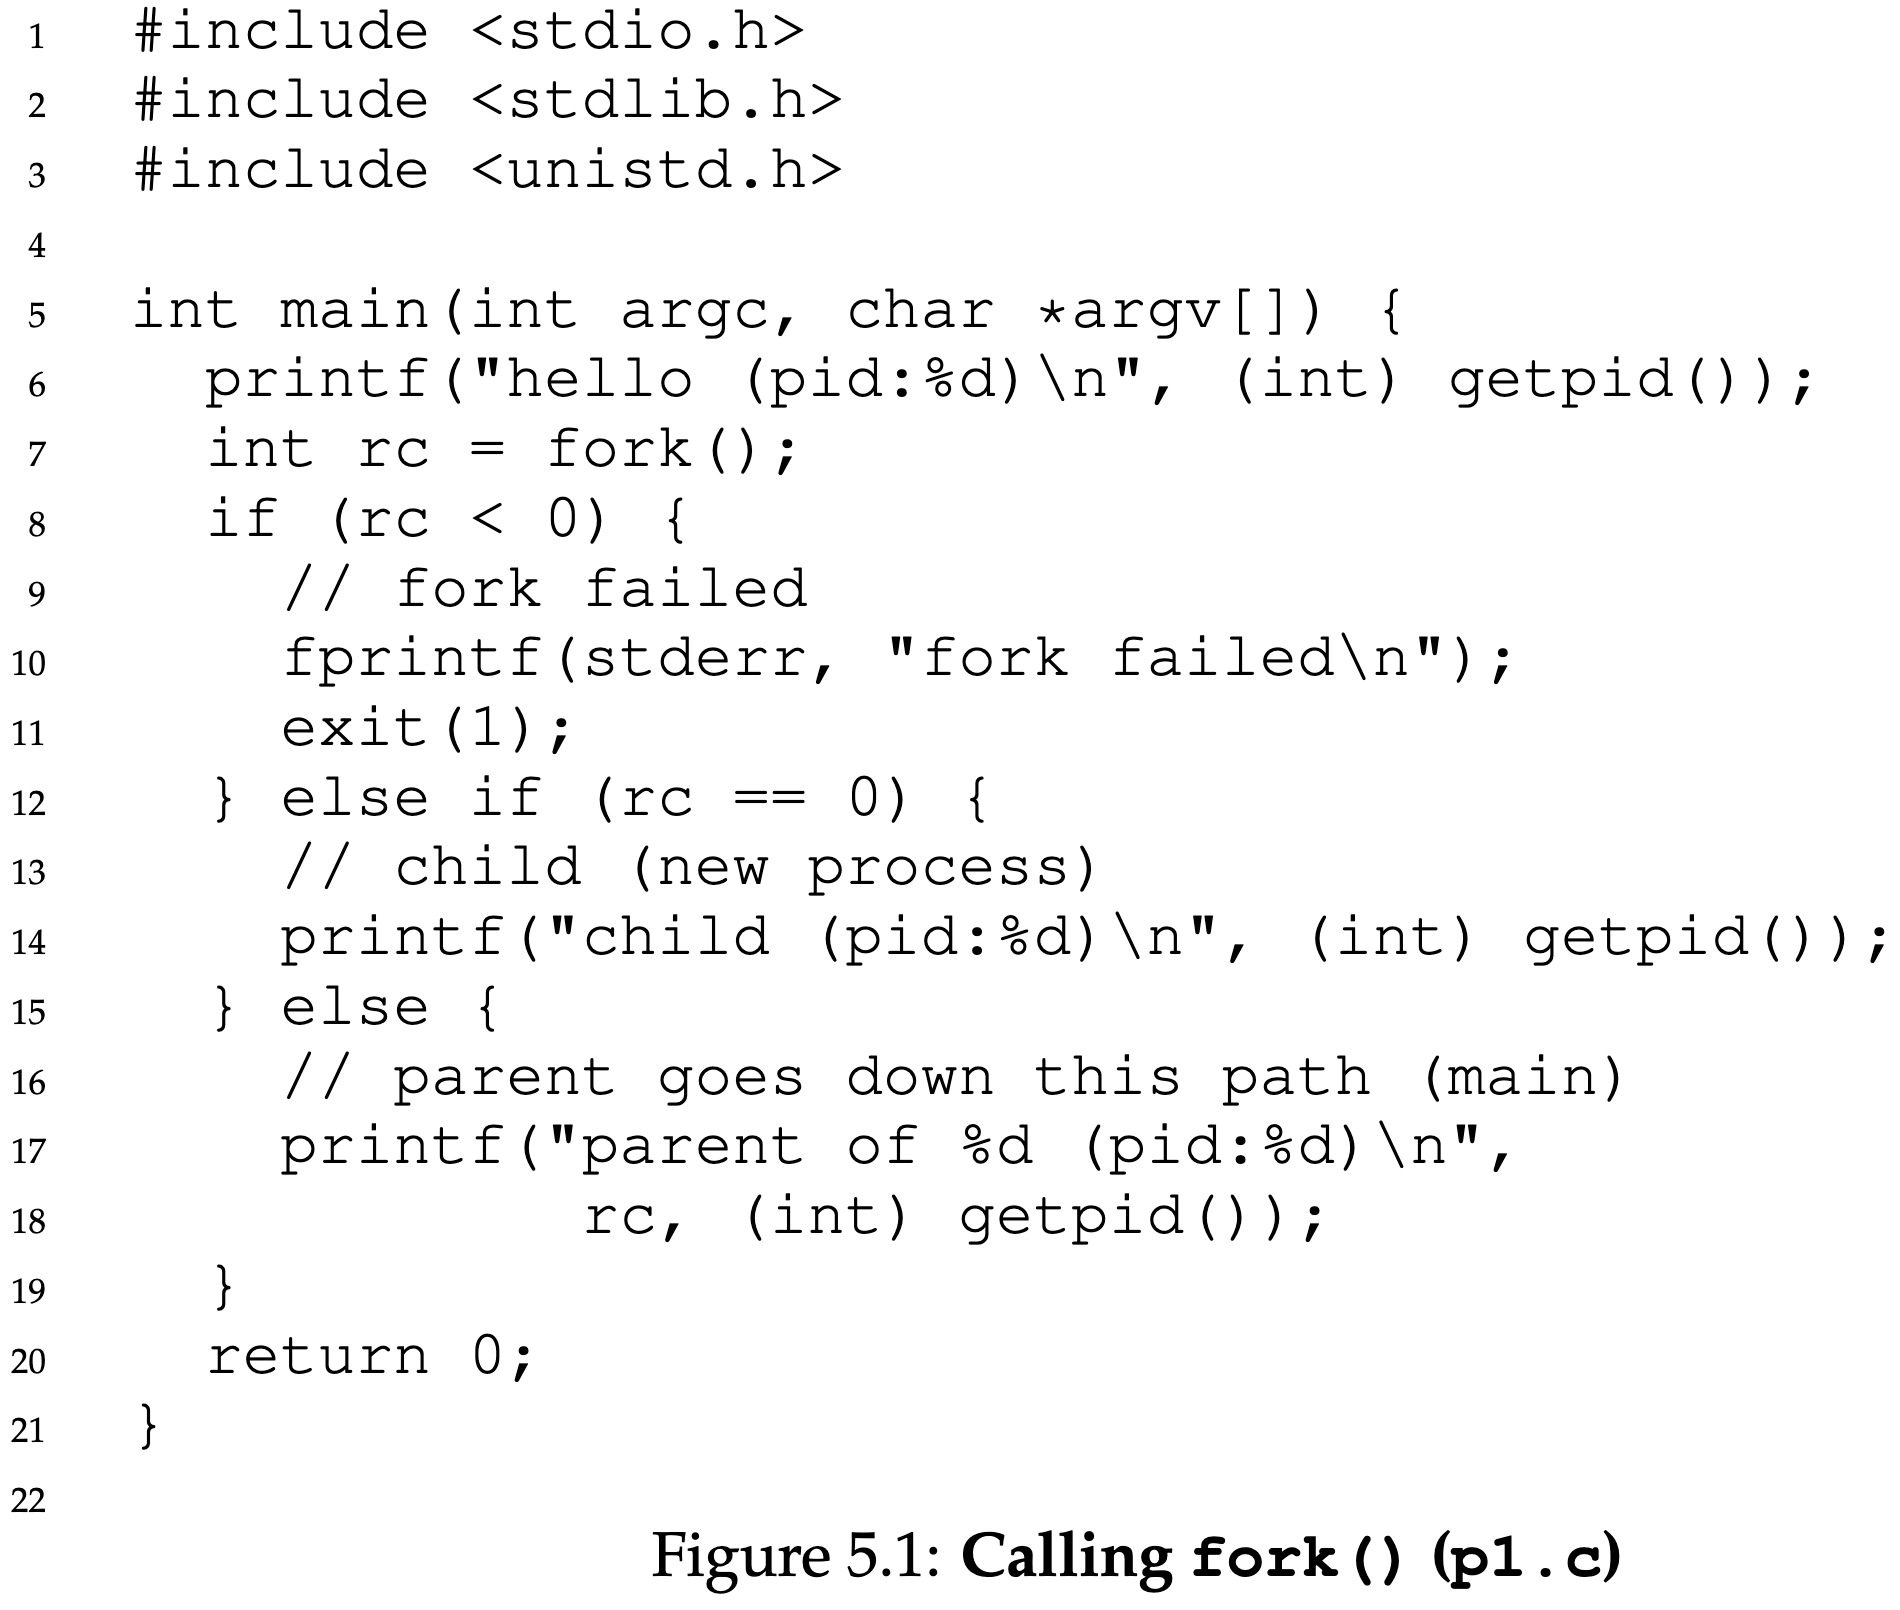
\includegraphics[width=1.1\linewidth]{figs/chapter-5/figure-5.1.png}
    \caption*{Source: chapter page 2.}
    \label{fig:figure-5.1}
\end{figure}
\end{column}

\end{columns}

\end{frame}

% ---------------------------------------------------------
\begin{frame}{Parent and Child Execution}

\begin{itemize}
    \item Each process has its own:
    \begin{itemize}
        \item address space;
        \item registers;
        \item program counter.
    \end{itemize}

    \item Parent and child may execute in different orders.
    \item The scheduler determines which process runs first.
    \item Execution after \texttt{fork()} is therefore
          \textbf{non-deterministic}.
\end{itemize}

\vspace{0.3cm}

\begin{block}{Process Identifier}
Each process is identified by a unique \textbf{PID}
(Process Identifier).
\end{block}

\end{frame}

% ---------------------------------------------------------
\begin{frame}{The \texttt{wait()} System Call}

\begin{columns}[T]

\begin{column}{0.45\textwidth}

\begin{itemize}
    \item A parent may need to wait for a child to finish.
    \item \texttt{wait()} blocks the parent.
    \item The parent becomes runnable again after the child terminates.
    \item This can make execution order predictable.
\end{itemize}

\vspace{0.2cm}

\begin{block}{Execution Order}
With \texttt{wait()}, the child completes before the parent continues
past the system call.
\end{block}

\end{column}

\begin{column}{0.52\textwidth}
\begin{figure}
    \centering
    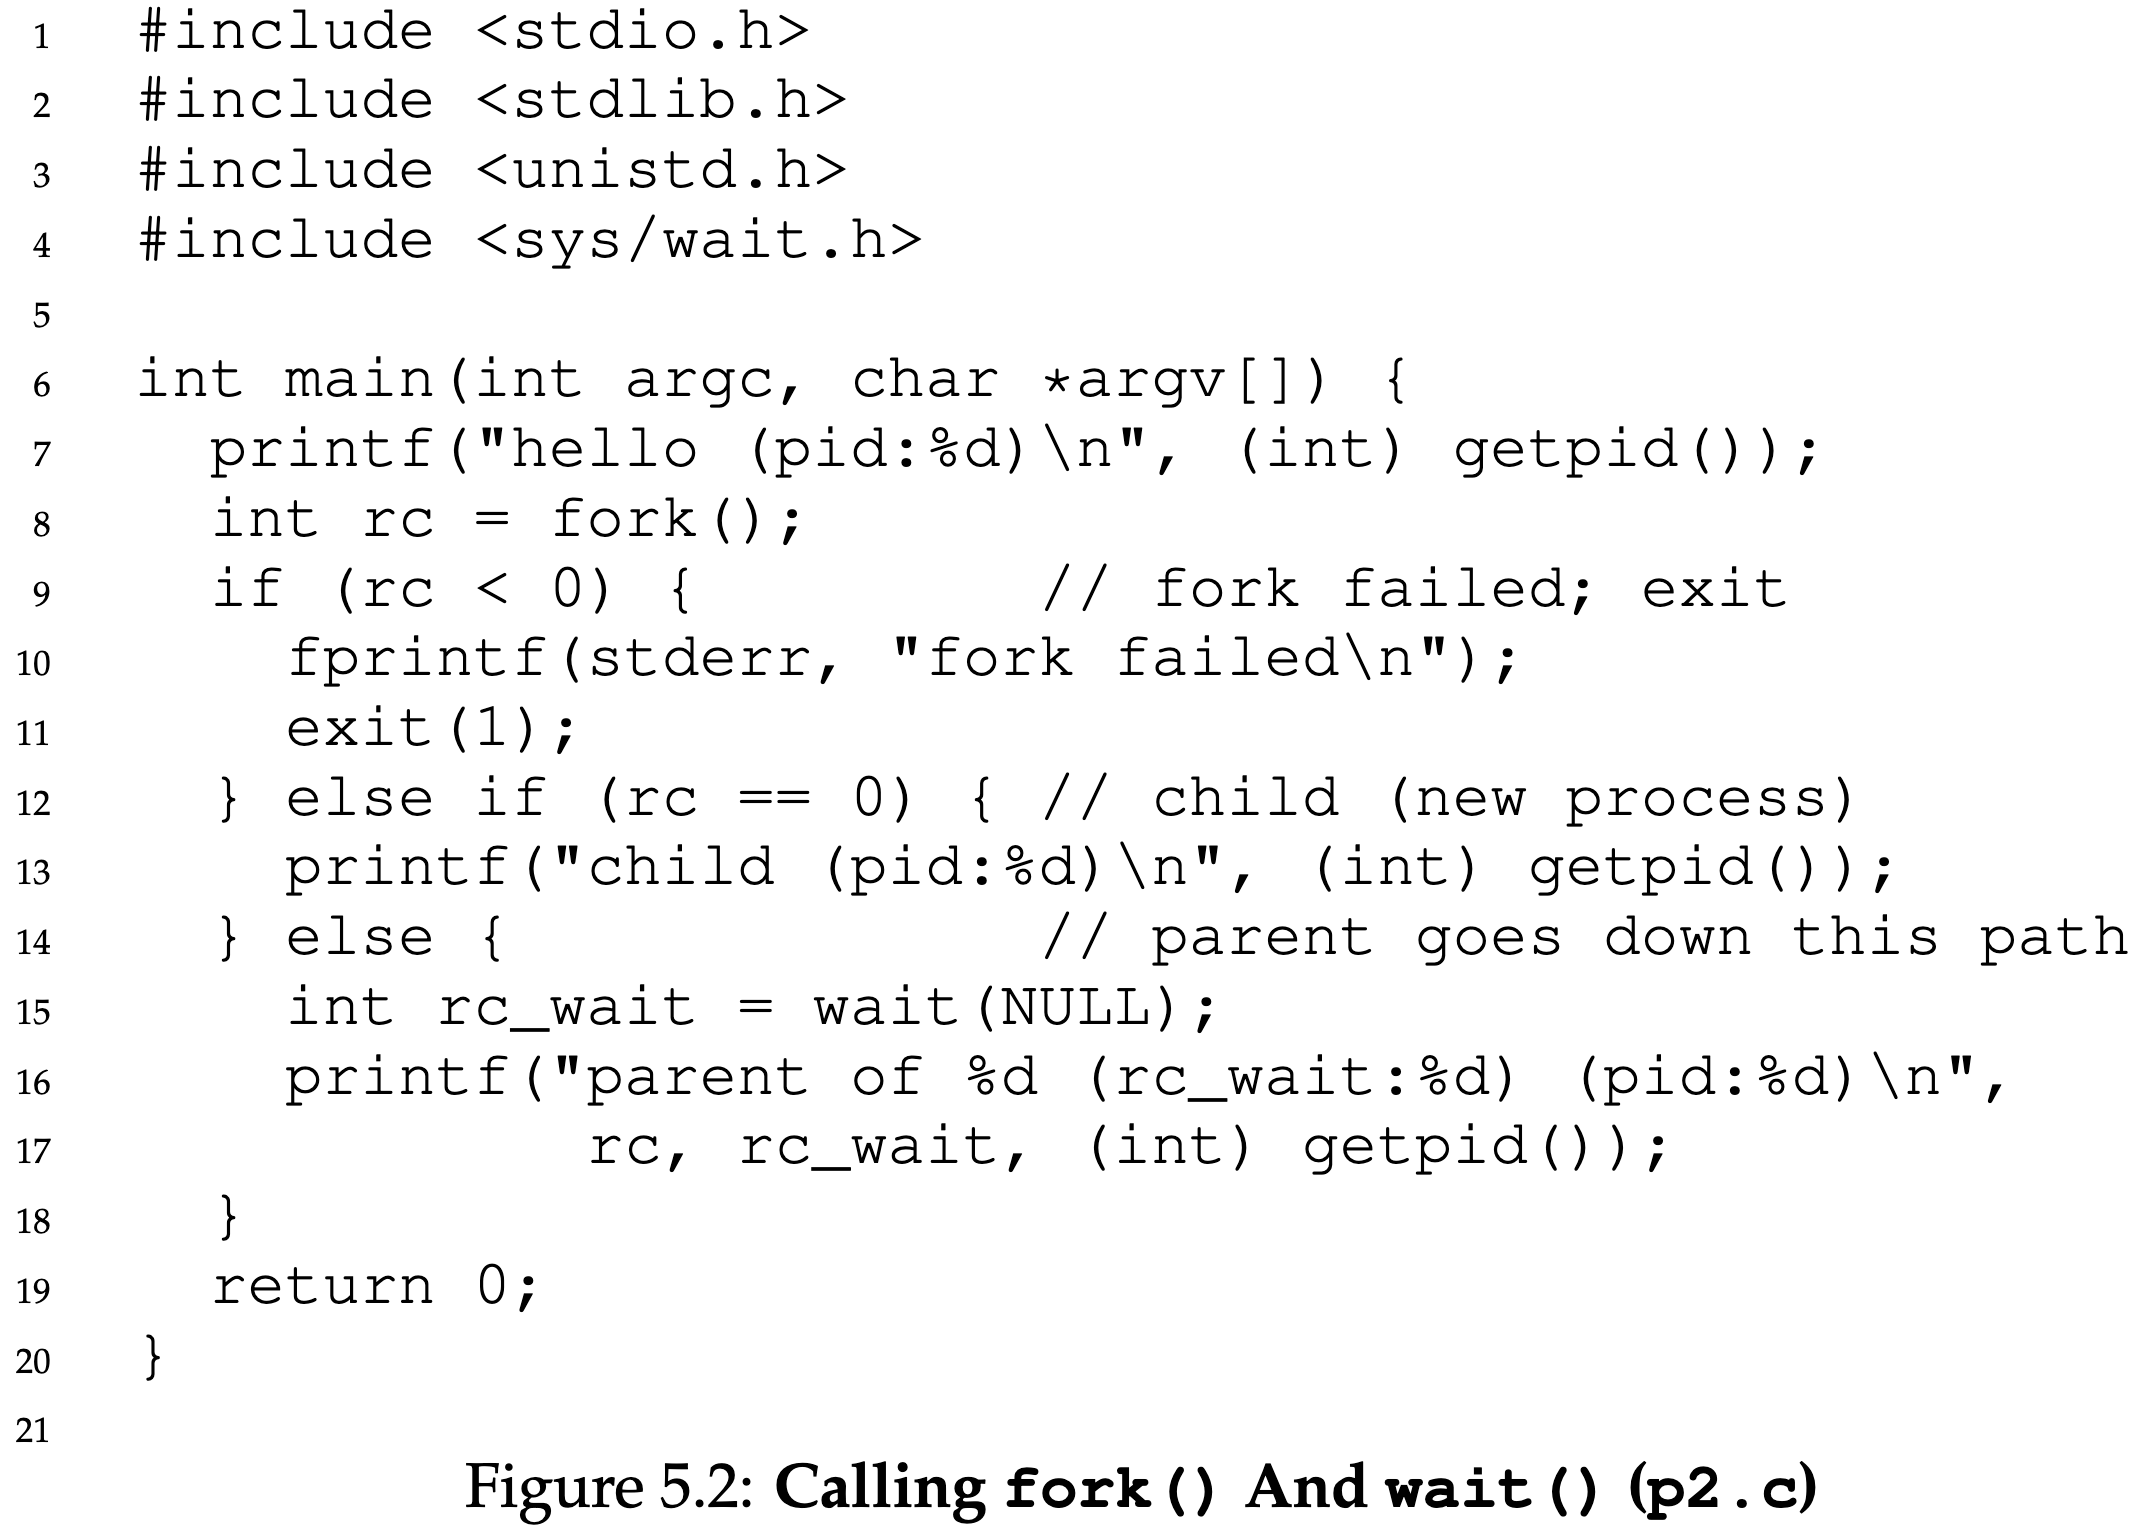
\includegraphics[width=1.1\linewidth]{figs/chapter-5/figure-5.2.png}
    \caption*{Source: chapter page 3.}
    \label{fig:figure-5.2}
\end{figure}
\end{column}

\end{columns}

\end{frame}

% ---------------------------------------------------------
\begin{frame}{The \texttt{exec()} System Call}

\begin{columns}[T]

\begin{column}{0.44\textwidth}

\begin{itemize}
    \item \texttt{exec()} runs a different program.
    \item It replaces the current process image.
    \item Code and static data are replaced.
    \item Heap and stack are re-initialized.
    \item It does \textbf{not} create a new process.
    \item A successful \texttt{exec()} does not return.
\end{itemize}

\end{column}

\begin{column}{0.53\textwidth}
\begin{figure}
    \centering
    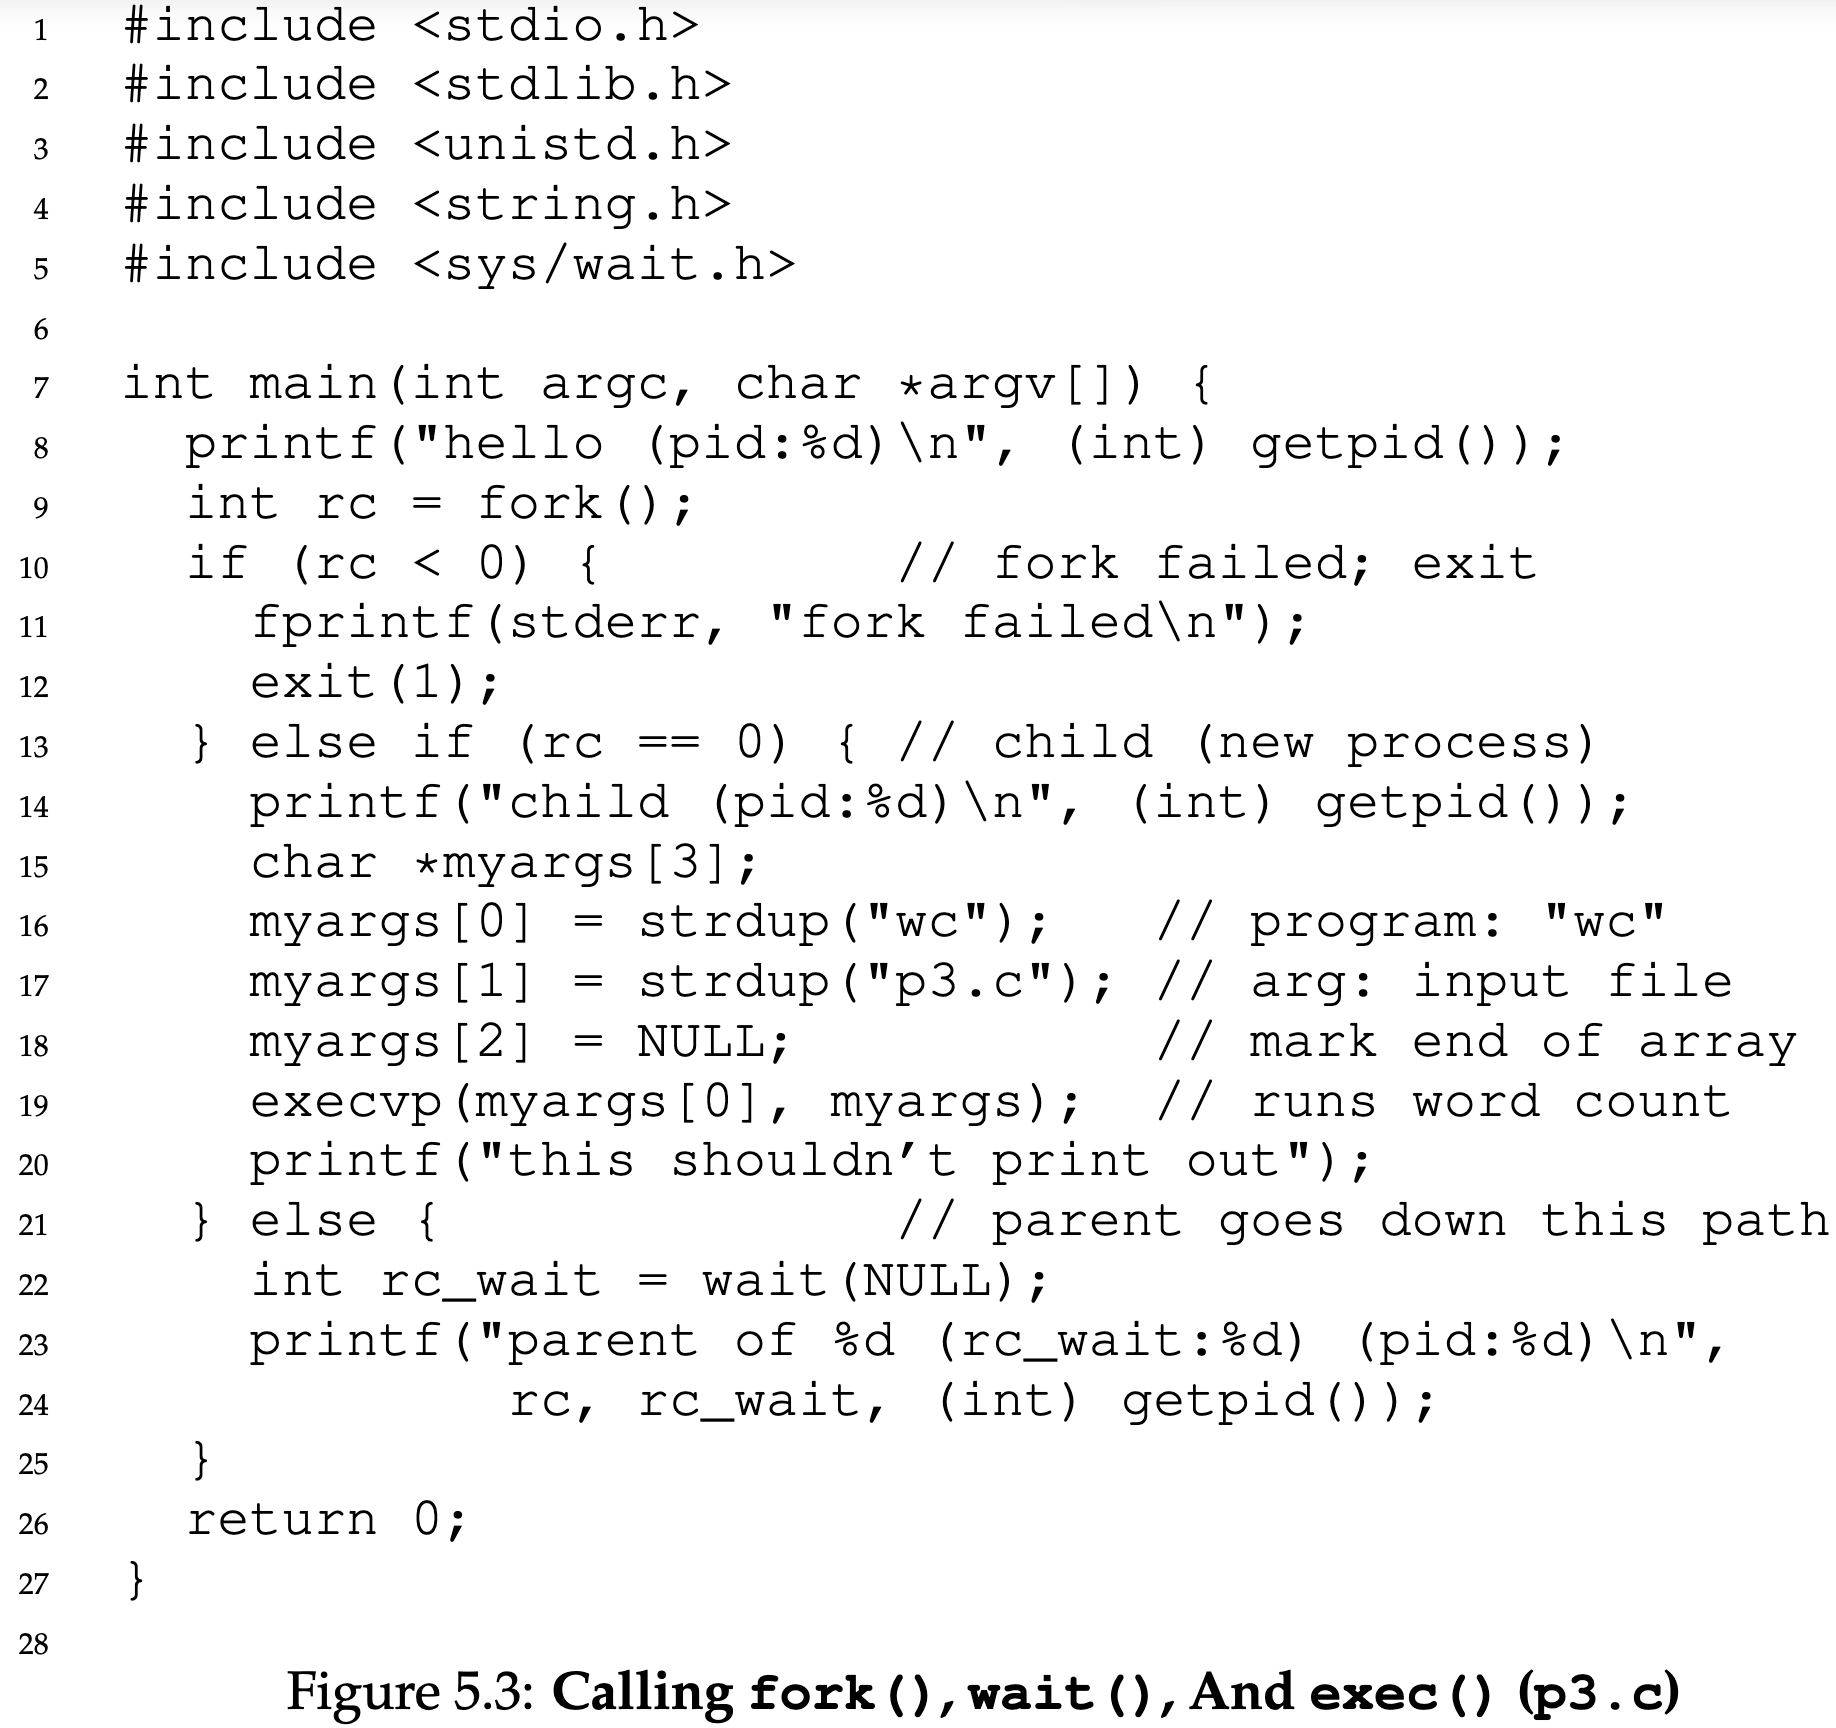
\includegraphics[width=1.1\linewidth]{figs/chapter-5/figure-5.3.png}
    \caption*{Source: chapter page 5.}
    \label{fig:figure-5.3}
\end{figure}
\end{column}

\end{columns}

\end{frame}

% ---------------------------------------------------------
\begin{frame}{Why Separate \texttt{fork()} and \texttt{exec()}?}

\begin{itemize}
    \item The separation is essential to the design of the UNIX shell.
    \item A shell typically:
    \begin{enumerate}
        \item reads a command;
        \item calls \texttt{fork()};
        \item modifies the child's environment if necessary;
        \item calls \texttt{exec()};
        \item waits for completion with \texttt{wait()}.
    \end{enumerate}
\end{itemize}

\vspace{0.3cm}

\begin{block}{Key Advantage}
The shell can perform operations \textbf{between}
\texttt{fork()} and \texttt{exec()}.
\end{block}

\end{frame}

% ---------------------------------------------------------
\begin{frame}[fragile]{I/O Redirection}

\begin{columns}[T]

\begin{column}{0.42\textwidth}

Example:

\begin{verbatim}
wc p3.c > newfile.txt
\end{verbatim}

\begin{itemize}
    \item The shell creates a child with \texttt{fork()}.
    \item The child closes standard output.
    \item It opens the destination file.
    \item The file becomes the new standard output.
    \item File descriptors remain open across \texttt{exec()}.
\end{itemize}

\end{column}

\begin{column}{0.55\textwidth}
\begin{figure}
    \centering
    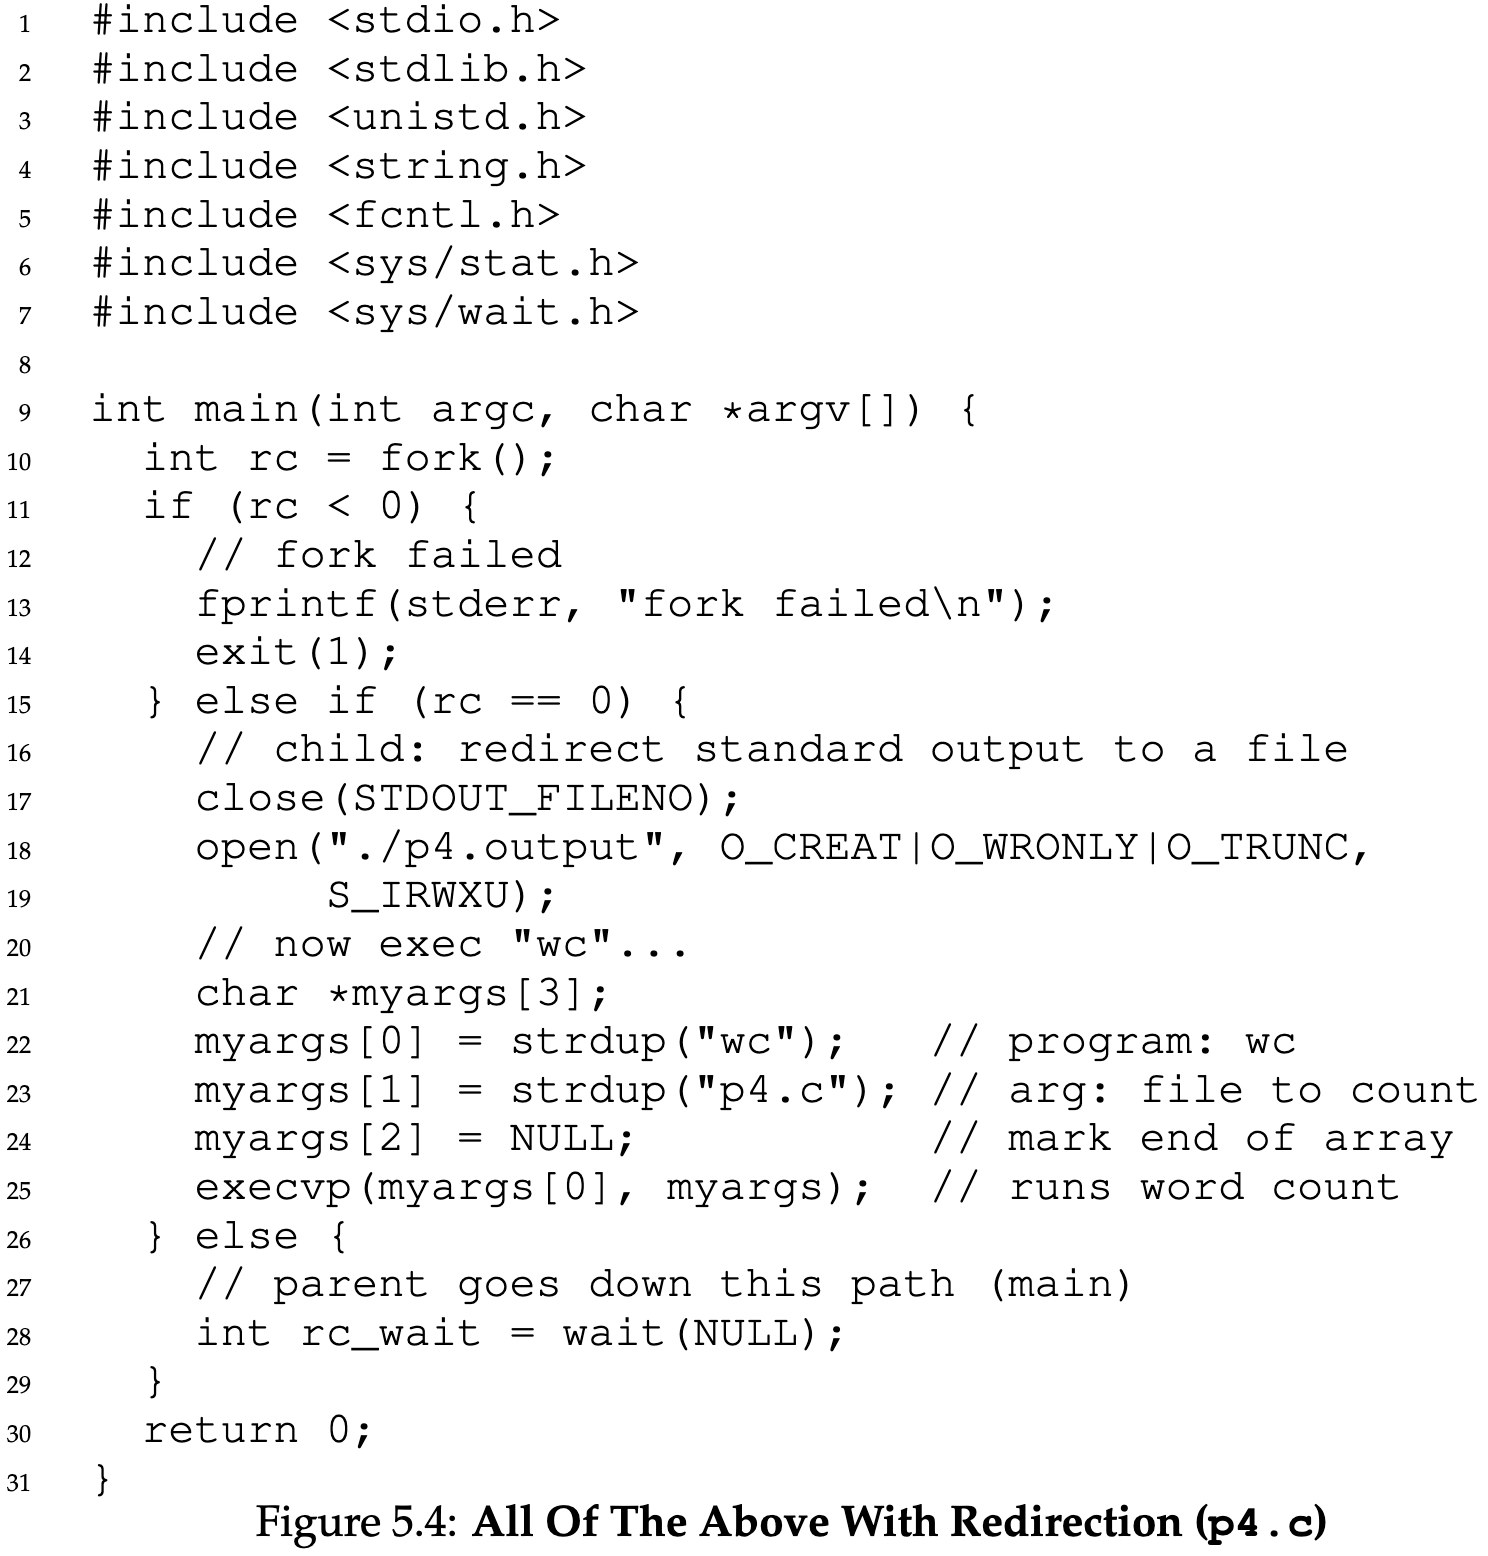
\includegraphics[width=1.1\linewidth]{figs/chapter-5/figure-5.4.png}
    \caption*{Source: chapter page 8.}
    \label{fig:figure-5.4}
\end{figure}
\end{column}

\end{columns}

\end{frame}

% ---------------------------------------------------------
\begin{frame}[fragile]{Pipes}

\begin{itemize}
    \item UNIX pipes use the \texttt{pipe()} system call.
    \item The output of one process is connected to an
          in-kernel pipe.
    \item The input of another process is connected to the same pipe.
    \item This allows commands to be combined into processing chains.
\end{itemize}

\vspace{0.3cm}

\begin{exampleblock}{Example}
\begin{verbatim}
grep -o foo file | wc -l
\end{verbatim}
\end{exampleblock}

The output of \texttt{grep} becomes the input of \texttt{wc}.

\end{frame}

% ---------------------------------------------------------
\begin{frame}{Process Control and Signals}

\begin{itemize}
    \item UNIX provides additional interfaces for process control.
    \item \texttt{kill()} sends signals to processes.
    \item Signals can stop, continue, interrupt, or terminate processes.
\end{itemize}

\vspace{0.2cm}

\begin{block}{Common Shell Shortcuts}
\begin{itemize}
    \item \texttt{Ctrl+C} $\rightarrow$ \texttt{SIGINT}
    \item \texttt{Ctrl+Z} $\rightarrow$ \texttt{SIGTSTP}
    \item \texttt{fg} can resume a stopped job.
\end{itemize}
\end{block}

\begin{itemize}
    \item Processes can use \texttt{signal()} to react to signals.
\end{itemize}

\end{frame}

% ---------------------------------------------------------
\begin{frame}{Users and Process Control}

\begin{itemize}
    \item UNIX systems support multiple users.
    \item Users generally control only their own processes.
    \item The operating system protects processes belonging to
          different users.
    \item The \textbf{superuser} (\texttt{root}) has broader privileges.
    \item Root can control processes belonging to other users.
\end{itemize}

\vspace{0.3cm}

\begin{alertblock}{Superuser}
Administrative privileges should be used carefully because they provide
extensive control over the system.
\end{alertblock}

\end{frame}

% ---------------------------------------------------------
\begin{frame}{Useful Process Tools}

\begin{itemize}
    \item \texttt{ps} -- displays running processes.
    \item \texttt{top} -- displays processes and resource usage.
    \item \texttt{kill} -- sends signals to processes.
    \item \texttt{killall} -- another interface for sending signals.
\end{itemize}

\vspace{0.3cm}

\begin{block}{Good Practice}
Use UNIX \texttt{man} pages to study system calls,
return values, options, and error conditions.
\end{block}

\end{frame}

% ---------------------------------------------------------
\begin{frame}{Process API: Summary}

\begin{itemize}
    \item \texttt{fork()} creates a new child process.
    \item \texttt{wait()} allows a parent to wait for a child.
    \item \texttt{exec()} replaces the current program with another.
    \item UNIX shells combine these mechanisms to execute commands.
    \item The separation of \texttt{fork()} and \texttt{exec()}
          enables redirection and pipes.
    \item Signals provide mechanisms for process control.
    \item Users and permissions determine which processes can be controlled.
\end{itemize}

\end{frame}
% =========================================================
% Section: Mechanism -- Limited Direct Execution
% =========================================================

\section{Direct Execution}

% ---------------------------------------------------------
\begin{frame}{CPU Virtualization: The Main Challenge}

\begin{block}{Goal}
The operating system must virtualize the CPU efficiently
while retaining control over the system.
\end{block}

\begin{itemize}
    \item The CPU is shared among multiple processes through
          \textbf{time sharing}.
    \item Two central challenges:
    \begin{itemize}
        \item \textbf{Performance}: minimize virtualization overhead.
        \item \textbf{Control}: prevent processes from taking over the system.
    \end{itemize}
    \item Hardware and operating-system support are both required.
\end{itemize}

\end{frame}

% ---------------------------------------------------------
\begin{frame}{Basic Technique (Mechanism): Limited Direct Execution}

\begin{itemize}
    \item The basic idea is to run programs \textbf{directly on the CPU}.
    \item Direct execution provides high performance.
    \item Before execution, the OS:
    \begin{itemize}
        \item creates a process entry;
        \item allocates memory;
        \item loads the program;
        \item prepares the stack;
        \item starts execution at the program entry point.
    \end{itemize}
\end{itemize}

\begin{alertblock}{Problem}
How can the OS run a program directly while still maintaining
control over the CPU?
\end{alertblock}

\end{frame}

% ---------------------------------------------------------
\begin{frame}{Direct Execution Without Limits}

\begin{columns}[T]
    \begin{column}{0.45\textwidth}
        \begin{itemize}
            \item The OS starts the program.
            \item The program executes directly on the processor.
            \item When it finishes, control returns to the OS.
        \end{itemize}

        \vspace{0.2cm}

        Two problems emerge:
        \begin{enumerate}
            \item How to restrict privileged operations?
            \item How to regain control of the CPU?
        \end{enumerate}
    \end{column}

    \begin{column}{0.52\textwidth}
    \begin{figure}
        \centering
        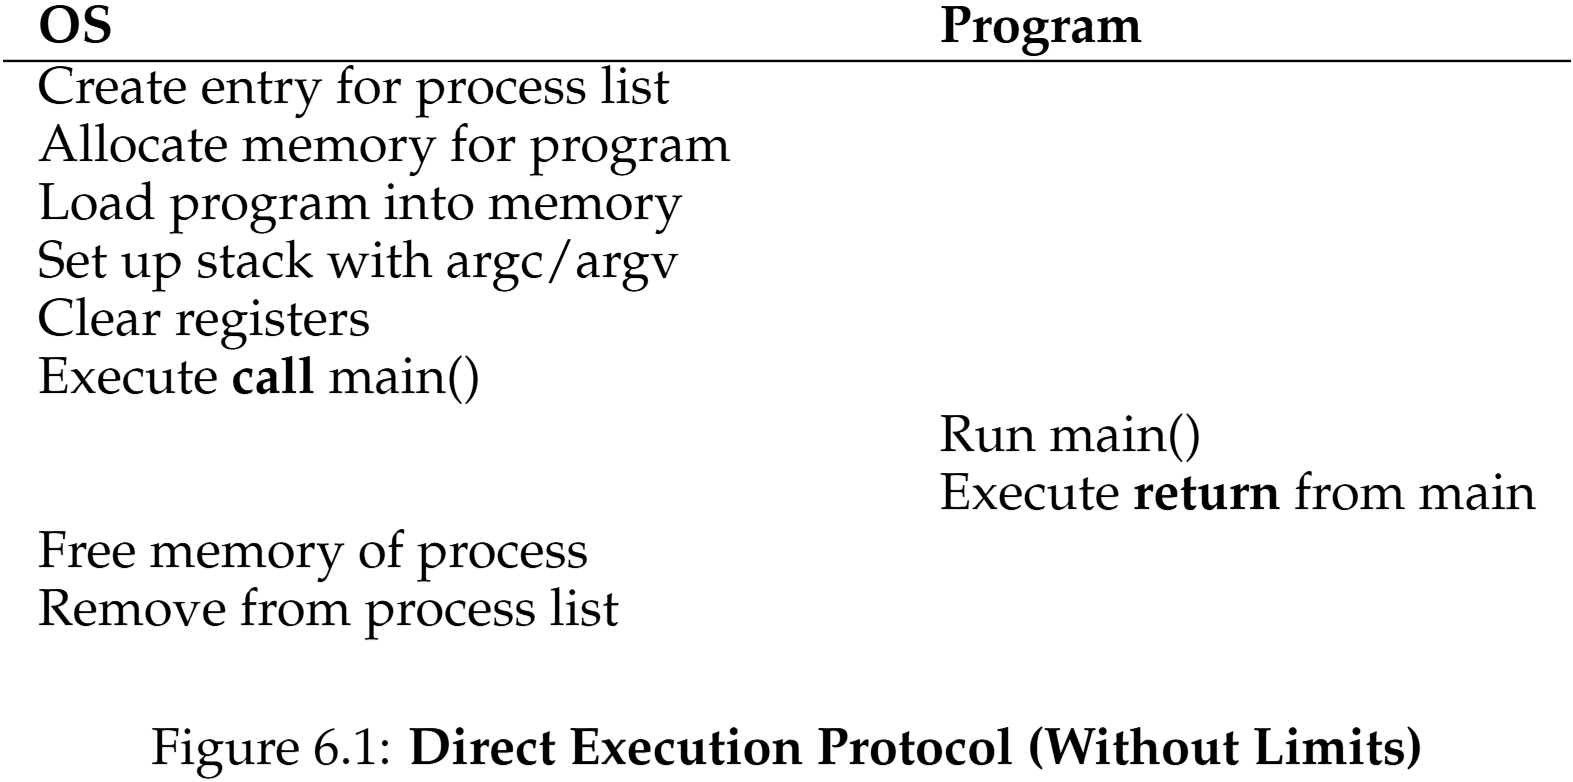
\includegraphics[width=1.1\linewidth]{figs/chapter-6/figure-6.1.png}
        \caption*{Source: chapter page 2.}
        \label{fig:figure-6.1}
    \end{figure}
    \end{column}
\end{columns}

\end{frame}

% ---------------------------------------------------------
\subsection*{Restricted Operations}

\begin{frame}{Problem \#1: Restricted Operations}

\begin{block}{The Crux}
A process must perform I/O and other restricted operations
without gaining complete control over the system.
\end{block}

\begin{itemize}
    \item Direct execution alone would allow applications to perform
          operations that should be controlled by the OS.
    \item The processor therefore supports different execution modes:
    \begin{itemize}
        \item \textbf{User mode}: restricted execution.
        \item \textbf{Kernel mode}: privileged execution.
    \end{itemize}
    \item Privileged operations are performed by the operating system.
\end{itemize}

\end{frame}

% ---------------------------------------------------------
\begin{frame}{System Calls and Protected Control Transfer}

\begin{itemize}
    \item User programs request OS services through
          \textbf{system calls}.
    \item A system call uses a special \textbf{trap instruction}.
    \item The trap:
    \begin{enumerate}
        \item saves the required processor state;
        \item switches execution to kernel mode;
        \item transfers control to a predefined OS handler.
    \end{enumerate}
    \item The OS performs the requested operation.
    \item A \textbf{return-from-trap} instruction restores execution
          in user mode.
\end{itemize}

\begin{block}{Key Idea}
System calls provide controlled access to privileged OS services.
\end{block}

\end{frame}

% ---------------------------------------------------------
\begin{frame}{Why System Calls Look Like Procedure Calls}

\begin{itemize}
    \item Calls such as \texttt{open()} and \texttt{read()} appear
          to be ordinary C procedure calls.
    \item The C library prepares:
    \begin{itemize}
        \item system-call arguments;
        \item the system-call number.
    \end{itemize}
    \item Library code then executes the hardware-specific
          \textbf{trap instruction}.
    \item After returning from the kernel, the library processes the
          return value and returns control to the application.
\end{itemize}

\end{frame}

% ---------------------------------------------------------
\begin{frame}{The Trap Table}

\begin{itemize}
    \item User programs cannot choose arbitrary kernel addresses
          as trap destinations.
    \item During boot, the OS initializes a \textbf{trap table}.
    \item The table defines handlers for events such as:
    \begin{itemize}
        \item system calls;
        \item hardware interrupts;
        \item exceptional conditions.
    \end{itemize}
    \item Installing the trap table is a
          \textbf{privileged operation}.
\end{itemize}

\begin{alertblock}{Protection}
User code requests a service through a system-call number,
rather than specifying an arbitrary kernel address.
\end{alertblock}

\end{frame}

% ---------------------------------------------------------
\begin{frame}{Limited Direct Execution Protocol}

\centering

\begin{figure}
    \centering
    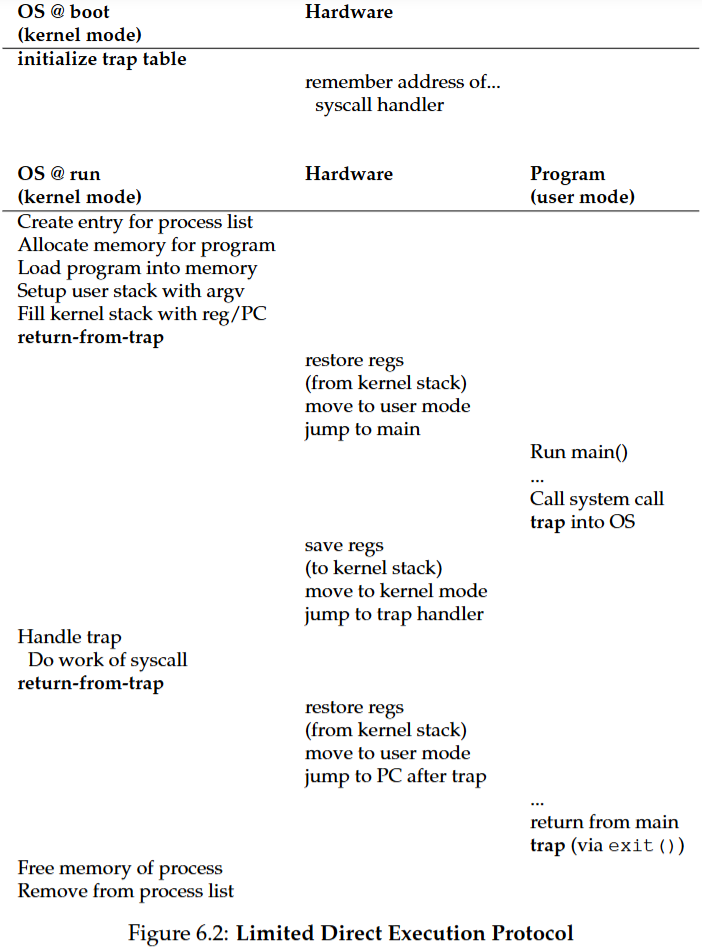
\includegraphics[width=0.5\linewidth]{figs/chapter-6/figure-6.2.png}
    \caption*{Source: chapter page 5.}
    \label{fig:figure-6.2}
\end{figure}

\end{frame}

% ---------------------------------------------------------
\subsection*{Regaining Control of the CPU}

\begin{frame}{Problem \#2: Switching Between Processes}

\begin{block}{The Crux}
How can the operating system regain control of the CPU
while a process is running?
\end{block}

\begin{itemize}
    \item If a user process is executing, the OS itself is not executing.
    \item The OS therefore needs a mechanism to regain control.
    \item Two approaches are discussed:
    \begin{itemize}
        \item cooperative;
        \item non-cooperative.
    \end{itemize}
\end{itemize}

\end{frame}

% ---------------------------------------------------------
\begin{frame}{Cooperative Approach}

\begin{itemize}
    \item The OS waits for the process to voluntarily transfer control.
    \item Control can return to the OS through:
    \begin{itemize}
        \item system calls;
        \item an explicit \texttt{yield()} system call;
        \item traps caused by illegal operations.
    \end{itemize}
\end{itemize}

\begin{alertblock}{Limitation}
A process running forever without making a system call
could monopolize the CPU.
\end{alertblock}

\end{frame}

% ---------------------------------------------------------
\begin{frame}{Non-Cooperative Approach: Timer Interrupt}

\begin{itemize}
    \item Hardware provides a programmable
          \textbf{timer interrupt}.
    \item The timer periodically interrupts the running process.
    \item When the interrupt occurs:
    \begin{enumerate}
        \item the running process is halted;
        \item its state is saved;
        \item the CPU switches to kernel mode;
        \item the OS interrupt handler executes.
    \end{enumerate}
    \item The OS has regained control of the CPU.
\end{itemize}

\begin{block}{Key Mechanism}
The timer interrupt prevents a process from monopolizing the CPU.
\end{block}

\end{frame}

% ---------------------------------------------------------
\subsection*{Context Switching}

\begin{frame}{Saving and Restoring Context}

\begin{itemize}
    \item After regaining control, the OS scheduler decides whether:
    \begin{itemize}
        \item to continue executing the current process; or
        \item to switch to another process.
    \end{itemize}

    \item A \textbf{context switch} saves the state of one process
          and restores the state of another.

    \item Relevant state includes:
    \begin{itemize}
        \item general-purpose registers;
        \item program counter;
        \item kernel stack pointer.
    \end{itemize}
\end{itemize}

\end{frame}

% ---------------------------------------------------------
\begin{frame}{Timer Interrupt and Context Switch}

\begin{columns}[T]
    \begin{column}{0.38\textwidth}
        \begin{itemize}
            \item Process A is executing.
            \item A timer interrupt occurs.
            \item Hardware saves A's user state.
            \item The OS enters the interrupt handler.
            \item The OS switches from A to B.
            \item B resumes execution.
        \end{itemize}
    \end{column}

    \begin{column}{0.60\textwidth}
    \begin{figure}
        \centering
        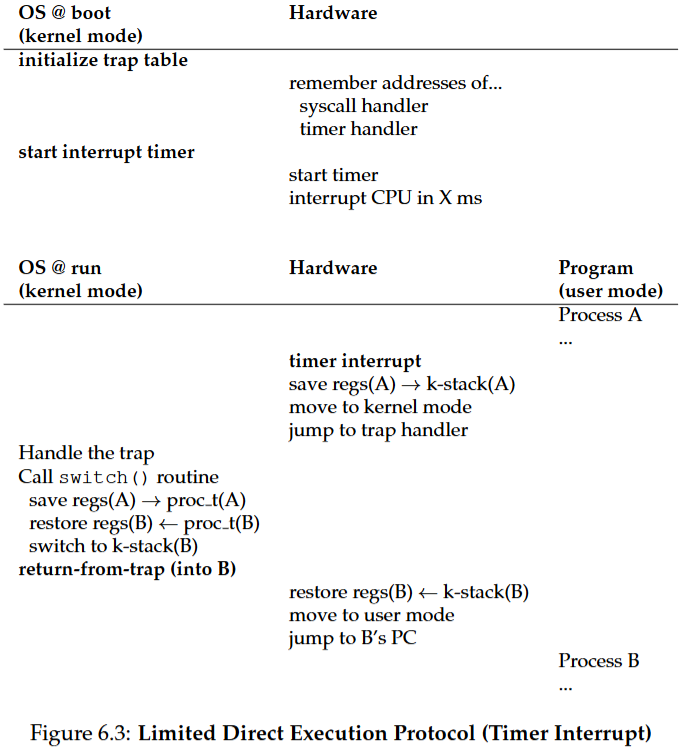
\includegraphics[width=0.9\linewidth]{figs/chapter-6/figure-6.3.png}
        \caption*{Source: chapter page 11.}
        \label{fig:figure-6.3}
    \end{figure}
    \end{column}
\end{columns}

\end{frame}

% ---------------------------------------------------------
\begin{frame}{Two Types of State Saving}

\begin{enumerate}
    \item \textbf{Hardware save/restore}
    \begin{itemize}
        \item occurs when the timer interrupt happens;
        \item saves the user registers;
        \item uses the process kernel stack.
    \end{itemize}

    \vspace{0.3cm}

    \item \textbf{Software save/restore}
    \begin{itemize}
        \item occurs during the context switch;
        \item performed explicitly by the OS;
        \item saves and restores kernel context.
    \end{itemize}
\end{enumerate}

\end{frame}

% ---------------------------------------------------------
\begin{frame}{Example: xv6 Context Switch}

\begin{columns}[T]
    \begin{column}{0.35\textwidth}
        \begin{itemize}
            \item Save registers of the old process.
            \item Restore registers of the new process.
            \item Switch the kernel stack.
            \item Return into the new execution context.
        \end{itemize}
    \end{column}

    \begin{column}{0.63\textwidth}
    \begin{figure}
        \centering
        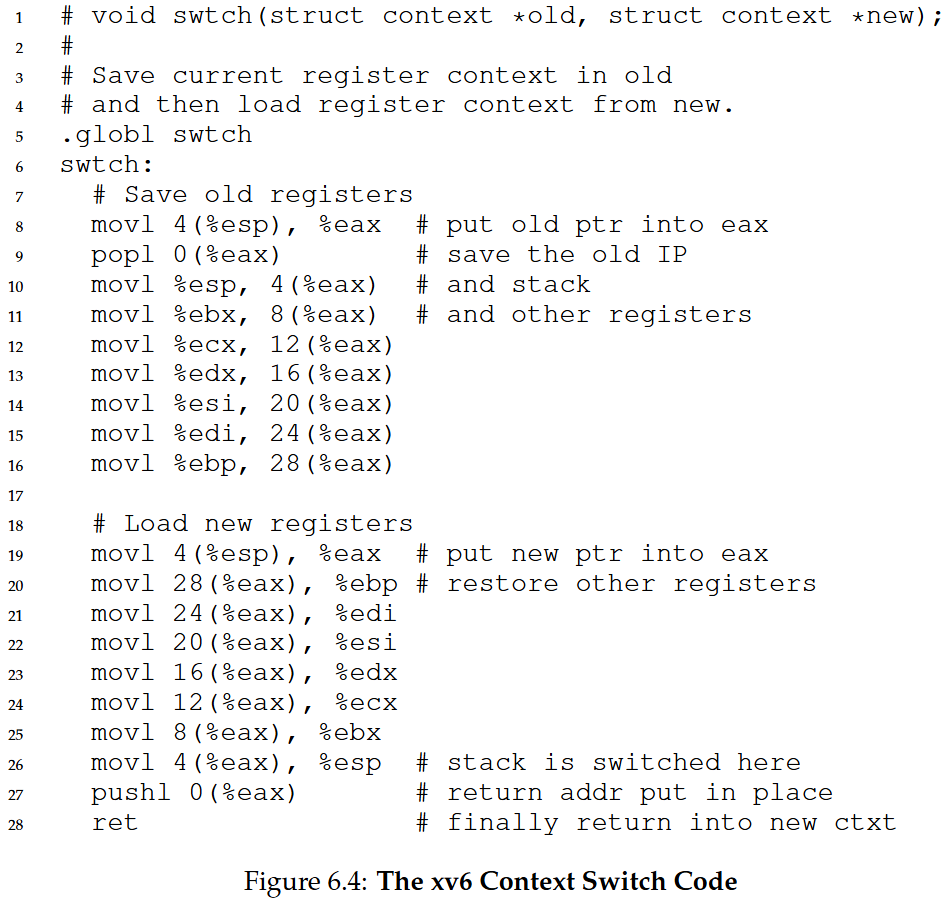
\includegraphics[width=1.1\linewidth]{figs/chapter-6/figure-6.4.png}
        \caption*{Source: chapter page 12.}
        \label{fig:figure-6.4}
    \end{figure}
    \end{column}
\end{columns}

\end{frame}

% ---------------------------------------------------------
\subsection*{Concurrency}

\begin{frame}{What About Concurrency?}

\begin{itemize}
    \item What happens if a timer interrupt occurs during a system call?
    \item What happens if another interrupt arrives while one is being handled?
\end{itemize}

\vspace{0.3cm}

The chapter briefly introduces two approaches:

\begin{itemize}
    \item temporarily disabling interrupts during interrupt processing;
    \item using locking mechanisms to protect kernel data structures.
\end{itemize}

\begin{block}{Next Step}
Detailed treatment of these problems belongs to the study of
\textbf{concurrency}.
\end{block}

\end{frame}

% ---------------------------------------------------------
\begin{frame}{Limited Direct Execution: Summary}

\begin{itemize}
    \item Programs execute directly on the CPU for high performance.
    \item \textbf{User mode} restricts application privileges.
    \item \textbf{Kernel mode} allows privileged operations.
    \item \textbf{System calls} use traps to enter the kernel safely.
    \item A \textbf{trap table} determines valid kernel entry points.
    \item A \textbf{timer interrupt} allows the OS to regain CPU control.
    \item A \textbf{context switch} changes the running process.
\end{itemize}

\begin{block}{Central Idea}
Limited direct execution combines efficient execution with
operating-system control.
\end{block}

\end{frame}

% ---------------------------------------------------------
\begin{frame}{Performance Measurement}

The chapter suggests measuring two fundamental operating-system costs:

\begin{itemize}
    \item \textbf{System-call cost}
    \begin{itemize}
        \item repeatedly execute a simple system call;
        \item measure total execution time;
        \item estimate the average cost per call.
    \end{itemize}

    \item \textbf{Context-switch cost}
    \begin{itemize}
        \item use two processes communicating through UNIX pipes;
        \item force repeated switches between the processes;
        \item measure the communication cycle.
    \end{itemize}
\end{itemize}

\begin{block}{Tools Mentioned in the Chapter}
\texttt{gettimeofday()}, \texttt{rdtsc}, \texttt{sched\_setaffinity()},
and \texttt{lmbench}.
\end{block}

\end{frame}

\begin{frame}{Direct Execution: Summary}

\begin{itemize}
    \item \textbf{Limited Direct Execution} combines performance and OS control.
    \item \textbf{User/kernel modes} restrict privileged operations.
    \item \textbf{System calls} use traps to safely enter the kernel.
    \item \textbf{Timer interrupts} allow the OS to regain CPU control.
    \item \textbf{Context switches} enable execution to move between processes.
\end{itemize}

\vspace{0.4cm}

\begin{block}{Next Step}
With these mechanisms in place, the remaining question is:

\begin{center}
\textbf{Which process should run at a given time?}
\end{center}

This is the responsibility of the \textbf{CPU scheduler}.
\end{block}

\end{frame}
% =========================================================
% SECTION: SCHEDULING
% =========================================================

\section{CPU Scheduling}

% ---------------------------------------------------------
\begin{frame}{From Mechanisms to Scheduling}

\begin{itemize}
    \item We now understand the low-level mechanisms for running processes:
    \begin{itemize}
        \item timer interrupts;
        \item context switching;
        \item switching between processes.
    \end{itemize}

    \item The next question concerns \textbf{policy}:
    \begin{itemize}
        \item Which process should run?
        \item When should it run?
        \item For how long?
    \end{itemize}
\end{itemize}

\begin{block}{The Crux}
How should we develop a basic framework for thinking about
\textbf{scheduling policies}?
\end{block}

\end{frame}

% ---------------------------------------------------------
\begin{frame}{Workload Assumptions}

To develop basic scheduling policies, we initially assume:

\begin{enumerate}
    \item Each job runs for the same amount of time.
    \item All jobs arrive at the same time.
    \item Once started, each job runs to completion.
    \item Jobs use only the CPU and perform no I/O.
    \item The run-time of each job is known.
\end{enumerate}

\medskip

These assumptions are intentionally unrealistic and will be
\textbf{relaxed progressively}.

\end{frame}

% ---------------------------------------------------------
\begin{frame}{Scheduling Metrics}

The main performance metric initially considered is
\textbf{turnaround time}:

\[
T_{\text{turnaround}}
=
T_{\text{completion}}
-
T_{\text{arrival}}
\]

With all jobs arriving at \(t=0\):

\[
T_{\text{turnaround}} = T_{\text{completion}}
\]

\begin{block}{Performance vs. Fairness}
Scheduling policies may improve performance at the cost of fairness,
or improve fairness at the cost of performance.
\end{block}

\end{frame}

% ---------------------------------------------------------
\begin{frame}{First In, First Out (FIFO)}

\begin{columns}[T]

\column{0.43\textwidth}

\begin{itemize}
    \item Also called \textbf{First Come, First Served (FCFS)}.
    \item Simple and easy to implement.
    \item Jobs execute in arrival order.
\end{itemize}

\medskip

Example:

\[
A = B = C = 10
\]

\[
\overline{T}_{turnaround}
=
\frac{10+20+30}{3}
=
20
\]

\column{0.55\textwidth}
\begin{figure}
    \centering
    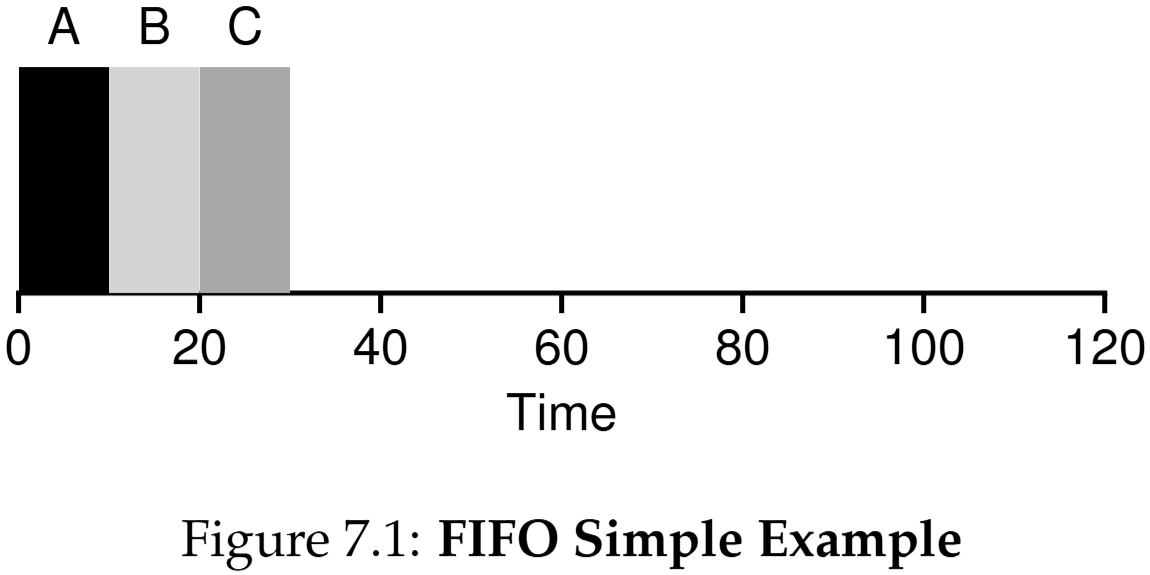
\includegraphics[width=1.1\linewidth]{figs/chapter-7/figure-7.1.png}
    \caption*{Source: chapter page 3.}
    \label{fig:figure-7.1}
\end{figure}
\end{columns}

\end{frame}

% ---------------------------------------------------------
\begin{frame}{The Convoy Effect}

Relax assumption 1: jobs may have \textbf{different lengths}.

\begin{columns}[T]

\column{0.43\textwidth}

Example:

\[
A=100,\qquad B=C=10
\]

Under FIFO:

\[
\overline{T}_{turnaround}
=
\frac{100+110+120}{3}
=
110
\]

\begin{block}{Convoy Effect}
Short jobs wait behind a long-running job.
\end{block}

\column{0.55\textwidth}
\begin{figure}
    \centering
    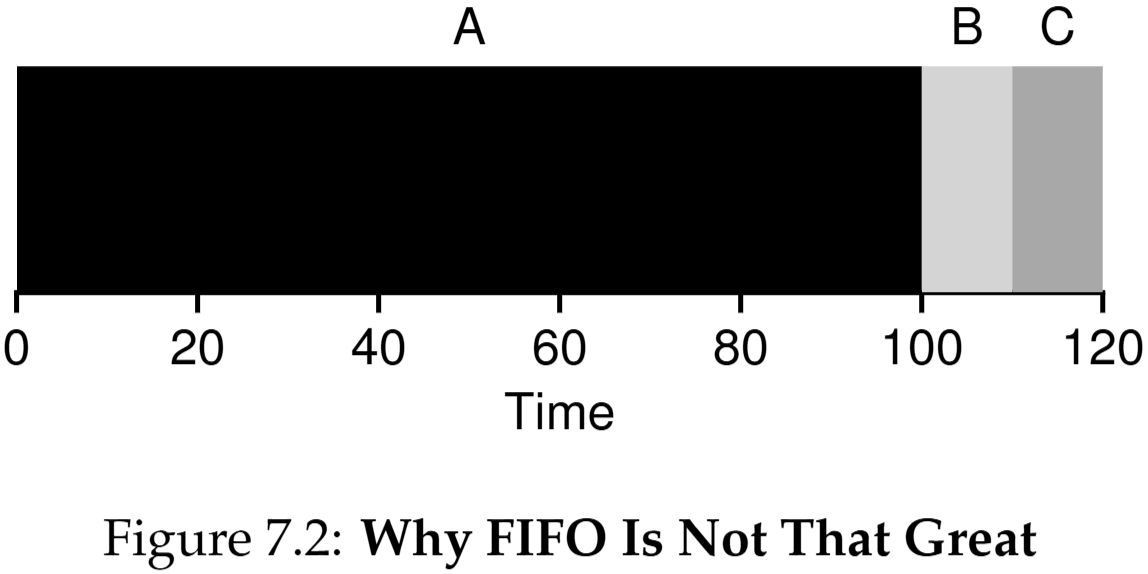
\includegraphics[width=1.1\linewidth]{figs/chapter-7/figure-7.2.png}
    \caption*{Source: chapter page 3.}
    \label{fig:figure-7.2}
\end{figure}
\end{columns}

\end{frame}

% ---------------------------------------------------------
\begin{frame}{Shortest Job First (SJF)}

\begin{columns}[T]

\column{0.43\textwidth}

\textbf{Shortest Job First (SJF)} executes jobs in increasing order
of run time.

\medskip

For:

\[
A=100,\qquad B=C=10
\]

SJF executes:

\[
B \rightarrow C \rightarrow A
\]

and obtains:

\[
\overline{T}_{turnaround}
=
\frac{10+20+120}{3}
=
50
\]

\column{0.55\textwidth}
\begin{figure}
    \centering
    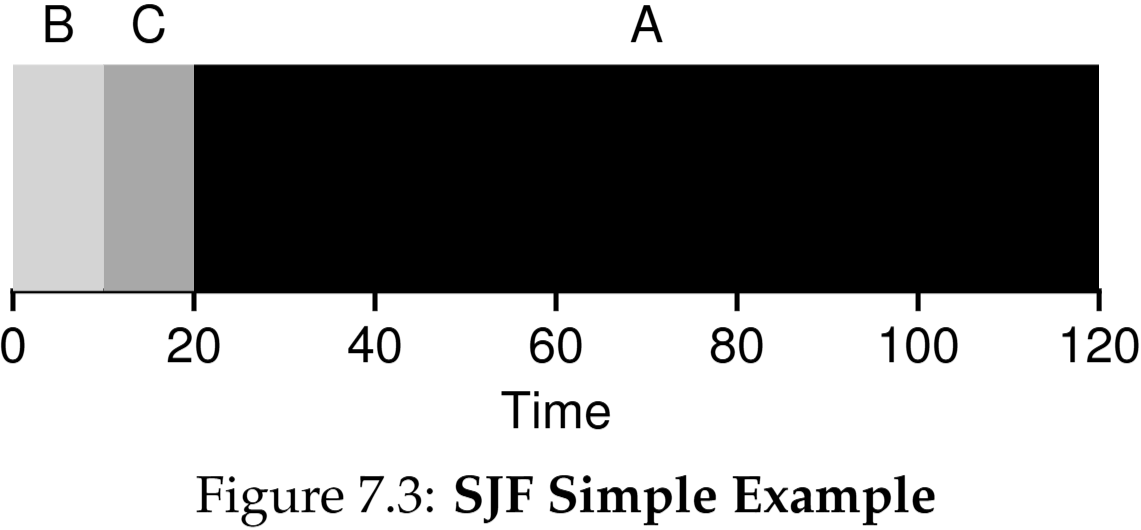
\includegraphics[width=1.1\linewidth]{figs/chapter-7/figure-7.3.png}
    \caption*{Source: chapter page 4.}
    \label{fig:figure-7.3}
\end{figure}
\end{columns}

\end{frame}

% ---------------------------------------------------------
\begin{frame}{SJF and Late Arrivals}

Now relax assumption 2: jobs may arrive at
\textbf{different times}.

\begin{columns}[T]

\column{0.43\textwidth}

Example:

\begin{itemize}
    \item \(A\) arrives at \(t=0\), requiring 100 s.
    \item \(B\) and \(C\) arrive at \(t=10\), requiring 10 s each.
\end{itemize}

Because SJF is non-preemptive, \(B\) and \(C\) must still wait for
\(A\).

\[
\overline{T}_{turnaround}=103.33
\]

\column{0.55\textwidth}
\begin{figure}
    \centering
    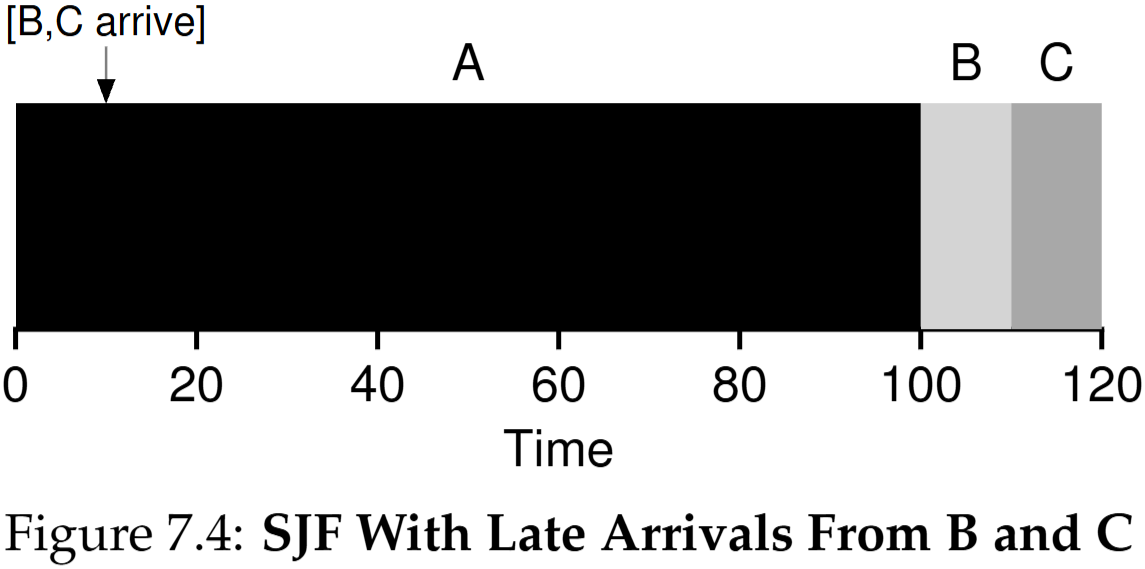
\includegraphics[width=1.1\linewidth]{figs/chapter-7/figure-7.4.png}
    \caption*{Source: chapter page 5.}
    \label{fig:figure-7.4}
\end{figure}
\end{columns}

\end{frame}

% ---------------------------------------------------------
\begin{frame}{Shortest Time-to-Completion First (STCF)}

Relax assumption 3: a running job may be
\textbf{preempted}.

\begin{columns}[T]

\column{0.43\textwidth}

\textbf{STCF} is the preemptive version of SJF.

\begin{itemize}
    \item When a new job arrives, compare the remaining execution times.
    \item Run the job with the least time remaining.
    \item A running process may therefore be preempted.
\end{itemize}

For the previous example:

\[
\overline{T}_{turnaround}=50
\]

\column{0.55\textwidth}
\begin{figure}
    \centering
    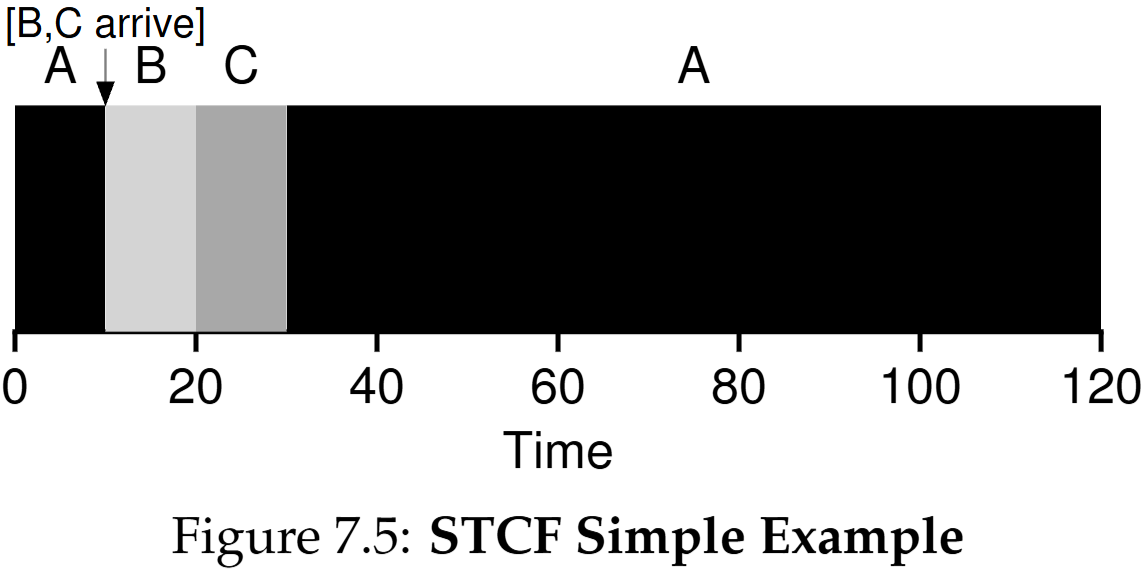
\includegraphics[width=1.1\linewidth]{figs/chapter-7/figure-7.5.png}
    \caption*{Source: chapter page 6.}
    \label{fig:figure-7.5}
\end{figure}
\end{columns}

\end{frame}

% ---------------------------------------------------------
\begin{frame}{A New Metric: Response Time}

Interactive systems require another metric:
\textbf{response time}.

\[
T_{\text{response}}
=
T_{\text{firstrun}}
-
T_{\text{arrival}}
\]

\begin{itemize}
    \item Turnaround time focuses on \textbf{completion}.
    \item Response time focuses on how quickly a job
          \textbf{starts receiving CPU time}.
    \item SJF/STCF may provide excellent turnaround time but poor
          interactive response.
\end{itemize}

\end{frame}

% ---------------------------------------------------------
\begin{frame}{SJF vs. Round Robin}

\begin{columns}[T]

\column{0.49\textwidth}

\centering

\textbf{SJF}

\vspace{0.2cm}

\begin{figure}
    \centering
    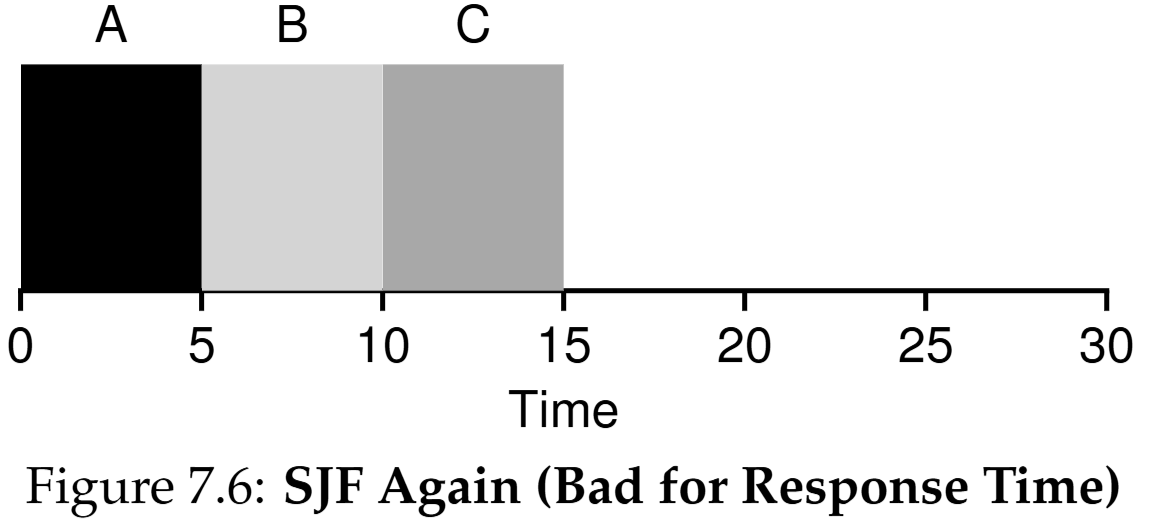
\includegraphics[width=1.1\linewidth]{figs/chapter-7/figure-7.6.png}
    \caption*{Source: chapter page 7.}
    \label{fig:figure-7.6}
\end{figure}

\[
\overline{T}_{response}
=
\frac{0+5+10}{3}=5
\]

\column{0.49\textwidth}

\centering

\textbf{Round Robin}

\vspace{0.2cm}

\begin{figure}
    \centering
    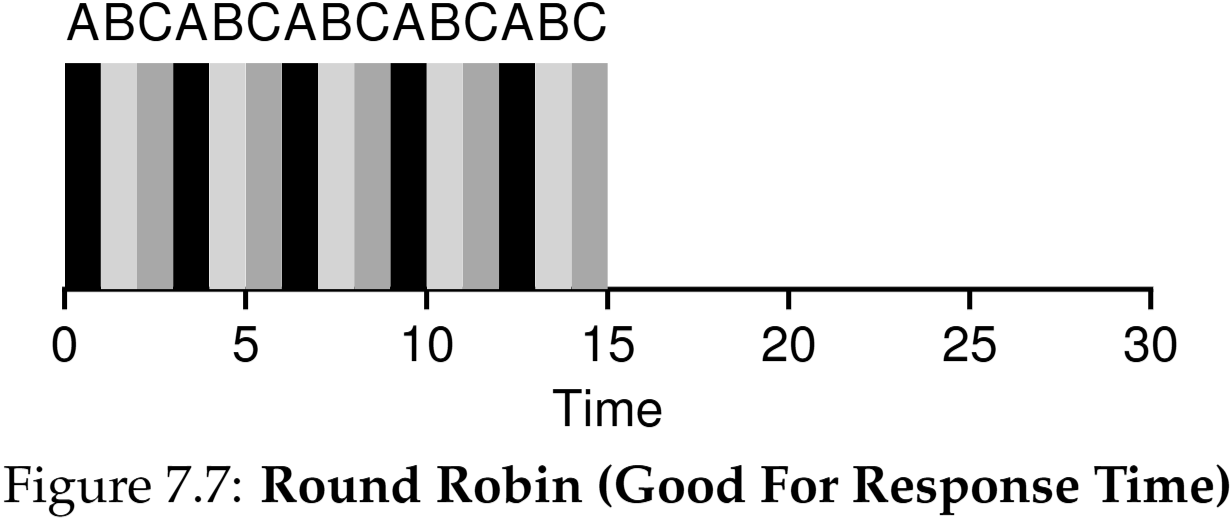
\includegraphics[width=1.1\linewidth]{figs/chapter-7/figure-7.7.png}
    \caption*{Source: chapter page 7.}
    \label{fig:figure-7.7}
\end{figure}

\[
\overline{T}_{response}
=
\frac{0+1+2}{3}=1
\]

\end{columns}

\end{frame}

% ---------------------------------------------------------
\begin{frame}{Round Robin (RR)}

Round Robin introduces \textbf{time slicing}.

\begin{itemize}
    \item Each job runs for a fixed \textbf{time slice} or
          \textbf{scheduling quantum}.
    \item After the quantum expires, the scheduler switches to the
          next job in the run queue.
    \item The process repeats until all jobs finish.
\end{itemize}

\begin{block}{Time-Slice Trade-off}
A shorter time slice improves response time, but increases the
relative cost of context switching.
\end{block}

\begin{itemize}
    \item Example: 10 ms quantum + 1 ms context switch
          \(\Rightarrow\) roughly 10\% switching overhead.
    \item Increasing the quantum amortizes this fixed cost.
\end{itemize}

\end{frame}

% ---------------------------------------------------------
\begin{frame}{Turnaround Time vs. Response Time}

The scheduling policies studied so far optimize different goals.

\begin{table}
\centering
\small

\begin{tabular}{lcc}
\hline
\textbf{Policy} &
\textbf{Turnaround} &
\textbf{Response} \\
\hline
FIFO      & workload-dependent & poor with convoy effect \\
SJF       & very good          & potentially poor \\
STCF      & very good          & potentially poor \\
RR        & poor               & very good \\
\hline
\end{tabular}

\end{table}

\begin{block}{Fundamental Trade-off}
Policies that divide CPU time fairly among active processes tend to
improve response time, but usually increase turnaround time.
\end{block}

\end{frame}

% ---------------------------------------------------------
\begin{frame}{Incorporating I/O}

Relax assumption 4: processes may perform \textbf{I/O}.

\begin{itemize}
    \item A process issuing I/O becomes blocked.
    \item The scheduler can run another process while the I/O proceeds.
    \item When the I/O completes, the blocked process becomes ready again.
\end{itemize}

\medskip

Example:

\begin{itemize}
    \item Job A: five 10-ms CPU bursts separated by I/O.
    \item Job B: one continuous 50-ms CPU burst.
\end{itemize}

\end{frame}

% ---------------------------------------------------------
\begin{frame}{Overlapping CPU and I/O}

\begin{columns}[T]

\column{0.49\textwidth}

\centering

\textbf{Poor Resource Use}

\vspace{0.2cm}

\begin{figure}
    \centering
    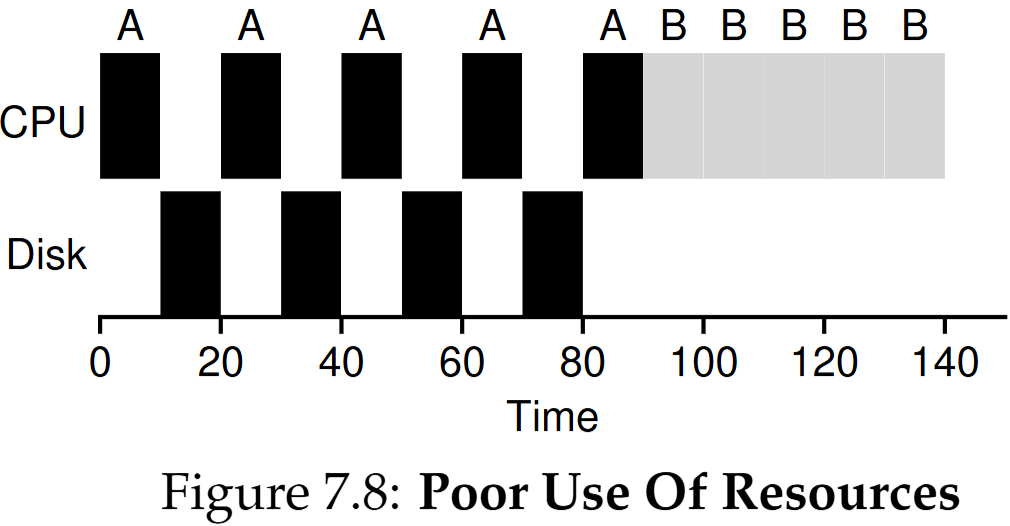
\includegraphics[width=1.1\linewidth]{figs/chapter-7/figure-7.8.png}
    \caption*{Source: chapter page 10.}
    \label{fig:figure-7.8}
\end{figure}

\column{0.49\textwidth}

\centering

\textbf{CPU/I/O Overlap}

\vspace{0.2cm}

\begin{figure}
    \centering
    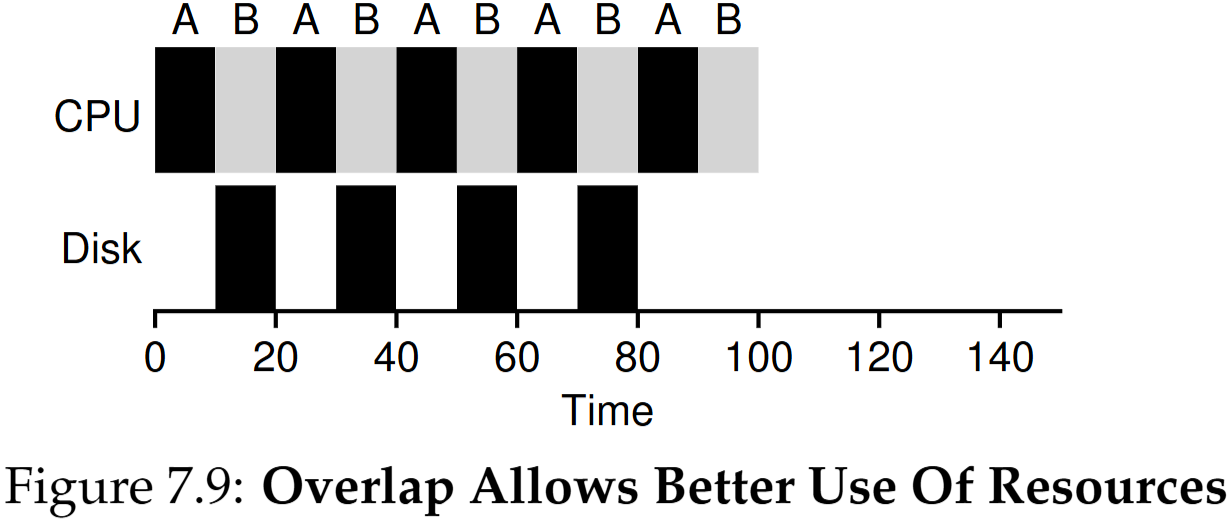
\includegraphics[width=1.1\linewidth]{figs/chapter-7/figure-7.9.png}
    \caption*{Source: chapter page 10.}
    \label{fig:figure-7.9}
\end{figure}

\end{columns}

\vspace{0.3cm}

\begin{block}{Key Idea}
Treating each CPU burst as a separate job enables CPU execution to
overlap with another process's I/O, improving system utilization.
\end{block}

\end{frame}

% ---------------------------------------------------------
\begin{frame}{No More Oracle}

One assumption still remains:

\begin{center}
\textbf{The scheduler knows the run-time of each job.}
\end{center}

In a general-purpose operating system, this information is normally
\textbf{not known in advance}.

\medskip

The remaining challenge is therefore:

\begin{itemize}
    \item obtain SJF/STCF-like turnaround behavior;
    \item preserve good response time;
    \item operate without knowing future job lengths.
\end{itemize}

\begin{block}{Next Step}
Use the \textbf{recent past to predict the future}:
the Multi-Level Feedback Queue (MLFQ).
\end{block}

\end{frame}

% ---------------------------------------------------------
\begin{frame}{CPU Scheduling: Summary}

\begin{itemize}
    \item Scheduling policy determines \textbf{which process runs}.
    \item \textbf{FIFO} is simple but may suffer from the convoy effect.
    \item \textbf{SJF/STCF} optimize turnaround time.
    \item \textbf{Round Robin} improves response time through time slicing.
    \item Response time and turnaround time represent an inherent
          scheduling trade-off.
    \item CPU and I/O can be overlapped to improve utilization.
    \item Real systems must schedule without knowing future job lengths.
\end{itemize}

\medskip

\begin{center}
\textbf{Next: Multi-Level Feedback Queue (MLFQ)}
\end{center}

\end{frame}
%------------------------------------------------
\section{Multi-Level Feedback Queue}
%------------------------------------------------

\begin{frame}{Multi-Level Feedback Queue (MLFQ)}
    \begin{itemize}
        \item MLFQ addresses two main scheduling goals:
        \begin{itemize}
            \item Minimize \textbf{turnaround time}.
            \item Minimize \textbf{response time} for interactive jobs.
        \end{itemize}

        \item Challenge:
        \begin{itemize}
            \item The OS usually does not know how long a job will run.
            \item SJF/STCF require such knowledge.
            \item Round Robin improves responsiveness but may hurt turnaround time.
        \end{itemize}
    \end{itemize}

    \begin{block}{The Crux}
        How can a scheduler achieve good response and turnaround times
        without a priori knowledge of job length?
    \end{block}
\end{frame}

%------------------------------------------------

\begin{frame}{Learning From History}
    \begin{itemize}
        \item MLFQ uses the \textbf{observed behavior} of jobs to determine priorities.
        \item It uses past behavior to predict future behavior.
        \item Interactive jobs tend to:
        \begin{itemize}
            \item run for short periods;
            \item frequently relinquish the CPU for I/O.
        \end{itemize}
        \item CPU-bound jobs tend to use the CPU for long periods.
    \end{itemize}
\end{frame}

%------------------------------------------------

\begin{frame}{MLFQ: Basic Structure}
    \begin{columns}
        \column{0.55\textwidth}
        \begin{itemize}
            \item MLFQ contains multiple queues with different priority levels.
            \item A ready job belongs to exactly one queue.
            \item Higher-priority jobs run before lower-priority jobs.
            \item Jobs at the same priority are scheduled using Round Robin.
        \end{itemize}

        \begin{block}{Basic Rules}
            \textbf{Rule 1:} If Priority(A) $>$ Priority(B), A runs.\\[0.3em]
            \textbf{Rule 2:} If Priority(A) = Priority(B), A and B run in RR.
        \end{block}

        \column{0.45\textwidth}
        \begin{figure}
            \centering
            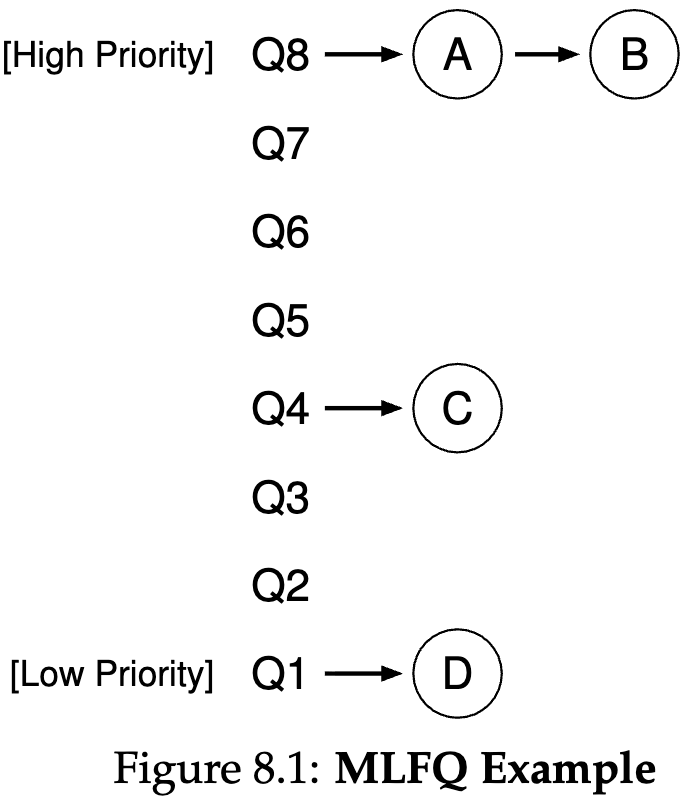
\includegraphics[width=1.1\linewidth]{figs/chapter-8/figure-8.1.png}
            \caption*{Source: chapter page 3.}
            \label{fig:figure-8.1}
        \end{figure}
    \end{columns}
\end{frame}

%------------------------------------------------

\begin{frame}{Changing Priority: First Attempt}
    \begin{itemize}
        \item A job's \textbf{allotment} is the amount of CPU time it may use
        at a priority level before being demoted.
        \item Initially, assume the allotment equals one time slice.
    \end{itemize}

    \begin{block}{Initial Priority Rules}
        \textbf{Rule 3:} A new job enters at the highest priority.\\[0.4em]

        \textbf{Rule 4a:} If a job uses its entire allotment, its priority is reduced.\\[0.4em]

        \textbf{Rule 4b:} If a job gives up the CPU before its allotment expires,
        it stays at the same priority.
    \end{block}
\end{frame}

%------------------------------------------------

\begin{frame}{Example 1: A Long-Running Job}
    \begin{columns}
        \column{0.48\textwidth}
        \begin{itemize}
            \item Consider three priority queues.
            \item Time slice: 10 ms.
            \item The job starts in the highest-priority queue.
            \item After consuming each allotment, it moves down one queue.
            \item Eventually, it remains in the lowest-priority queue.
        \end{itemize}

        \column{0.52\textwidth}
        \begin{figure}
            \centering
            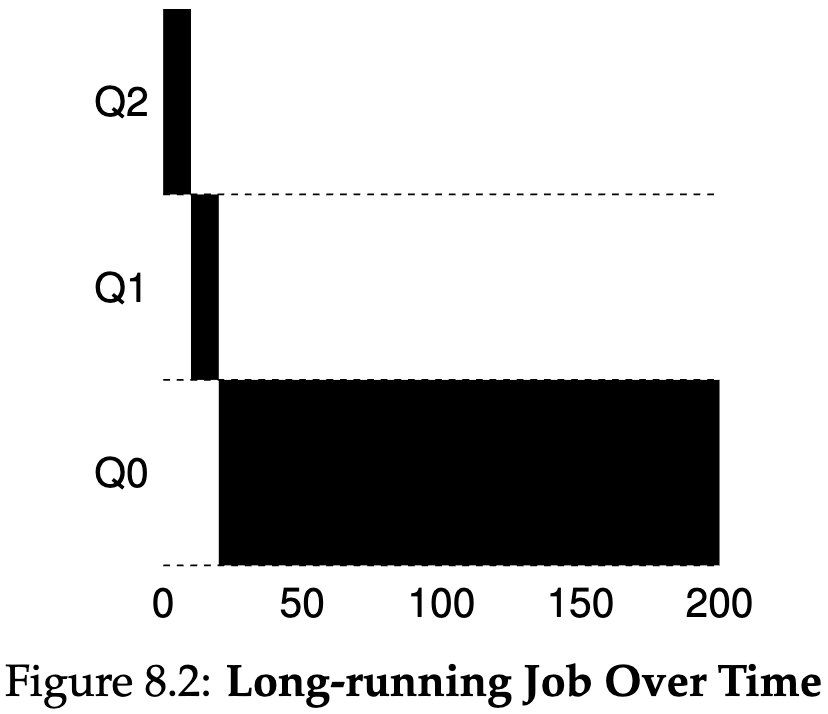
\includegraphics[width=1.1\linewidth]{figs/chapter-8/figure-8.2.png}
            \caption*{Source: chapter page 4.}
            \label{fig:figure-8.2}
        \end{figure}
    \end{columns}
\end{frame}

%------------------------------------------------

\begin{frame}{Example 2: A Short Job Arrives}
    \begin{columns}
        \column{0.48\textwidth}
        \begin{itemize}
            \item Job A is a long-running CPU-intensive job.
            \item Job B is a newly-arrived short job.
            \item B enters at the highest priority.
            \item Because B is short, it completes before reaching the lowest queue.
            \item MLFQ therefore approximates SJF without knowing job lengths.
        \end{itemize}

        \column{0.52\textwidth}
        \begin{figure}
            \centering
            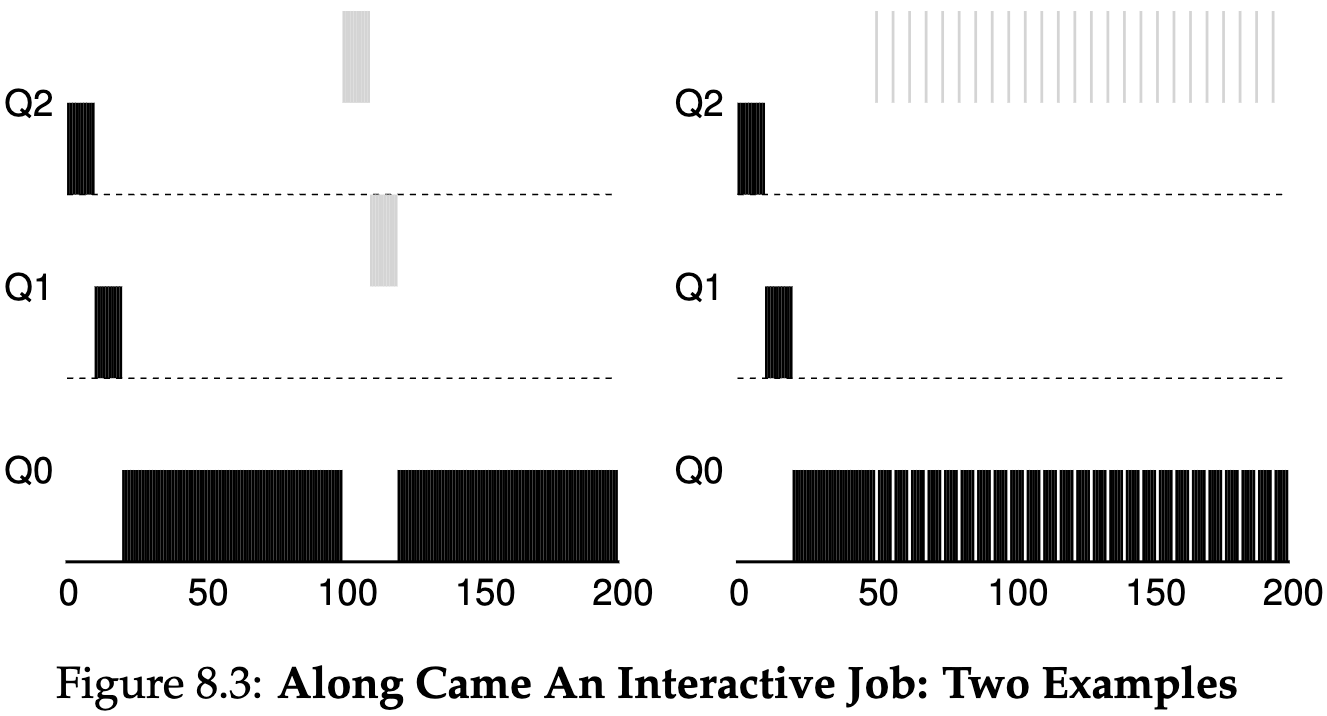
\includegraphics[width=1.1\linewidth]{figs/chapter-8/figure-8.3.png}
            \caption*{Source: chapter page 5.}
            \label{fig:figure-8.3-left}
        \end{figure}
    \end{columns}
\end{frame}

%------------------------------------------------

\begin{frame}{Example 3: Interactive Jobs and I/O}
    \begin{columns}
        \column{0.48\textwidth}
        \begin{itemize}
            \item Interactive jobs often relinquish the CPU for I/O.
            \item Under Rule 4b, such jobs remain at high priority.
            \item This allows interactive jobs to receive fast CPU service.
        \end{itemize}

        \column{0.52\textwidth}
        \begin{figure}
            \centering
            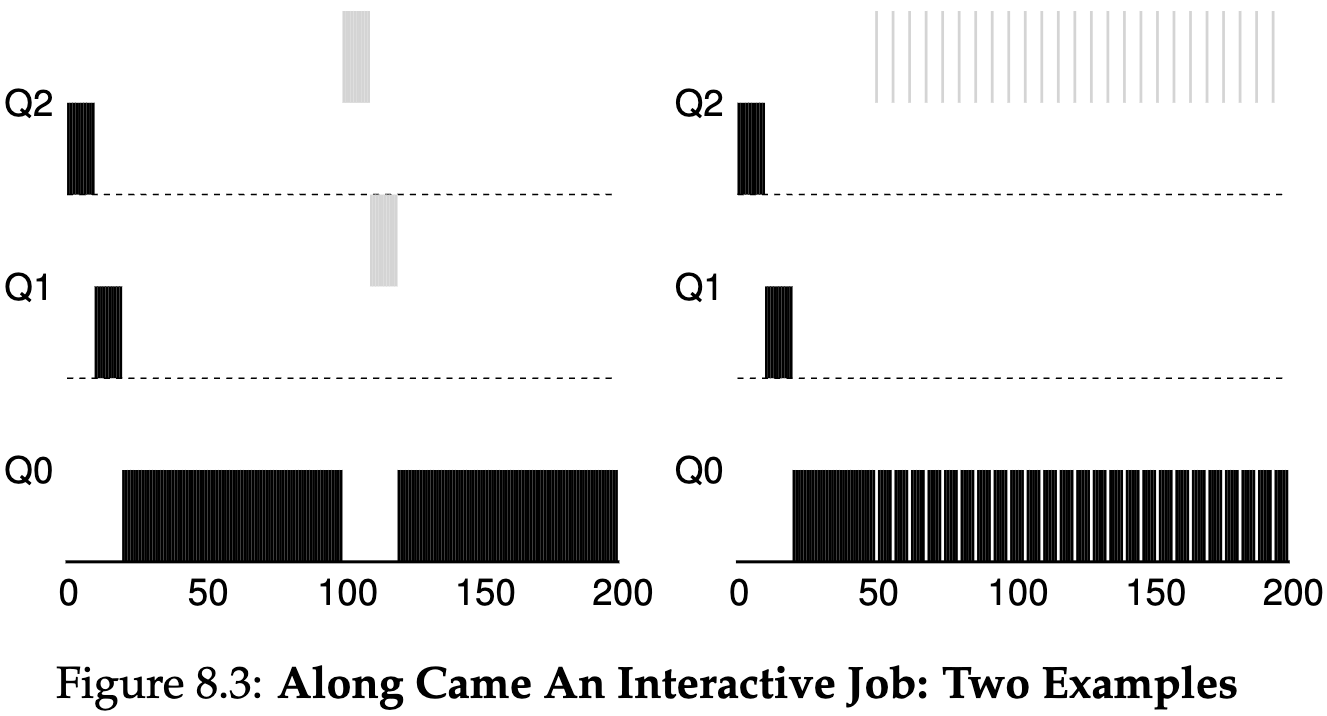
\includegraphics[width=1.1\linewidth]{figs/chapter-8/figure-8.3.png}
            \caption*{Source: chapter page 5.}
            \label{fig:figure-8.3-rigth}
        \end{figure}
    \end{columns}
\end{frame}

%------------------------------------------------

\begin{frame}{Problems With the Initial MLFQ}
    \begin{enumerate}
        \item \textbf{Starvation}
        \begin{itemize}
            \item Too many interactive jobs may consume all CPU time.
            \item Long-running jobs may never execute.
        \end{itemize}

        \item \textbf{Gaming the Scheduler}
        \begin{itemize}
            \item A job can issue I/O just before its allotment expires.
            \item It can remain at high priority and obtain an unfair CPU share.
        \end{itemize}

        \item \textbf{Changing Behavior}
        \begin{itemize}
            \item A CPU-bound process may later become interactive.
            \item The current rules do not adapt well to this change.
        \end{itemize}
    \end{enumerate}
\end{frame}

%------------------------------------------------

\begin{frame}{Attempt \#2: Priority Boost}
    \begin{block}{Rule 5}
        After some time period $S$, move all jobs in the system
        to the topmost queue.
    \end{block}

    \begin{itemize}
        \item Prevents starvation of long-running jobs.
        \item Allows jobs whose behavior changed to regain high priority.
        \item However, choosing a proper value for $S$ is difficult.
    \end{itemize}
\end{frame}

%------------------------------------------------

\begin{frame}{Priority Boost in Action}
    \begin{columns}
        \column{0.45\textwidth}
        \begin{itemize}
            \item Without priority boosts:
            \begin{itemize}
                \item a long-running job may starve.
            \end{itemize}

            \item With periodic boosts:
            \begin{itemize}
                \item the long-running job periodically receives CPU time.
            \end{itemize}
        \end{itemize}

        \column{0.55\textwidth}
        \begin{figure}
            \centering
            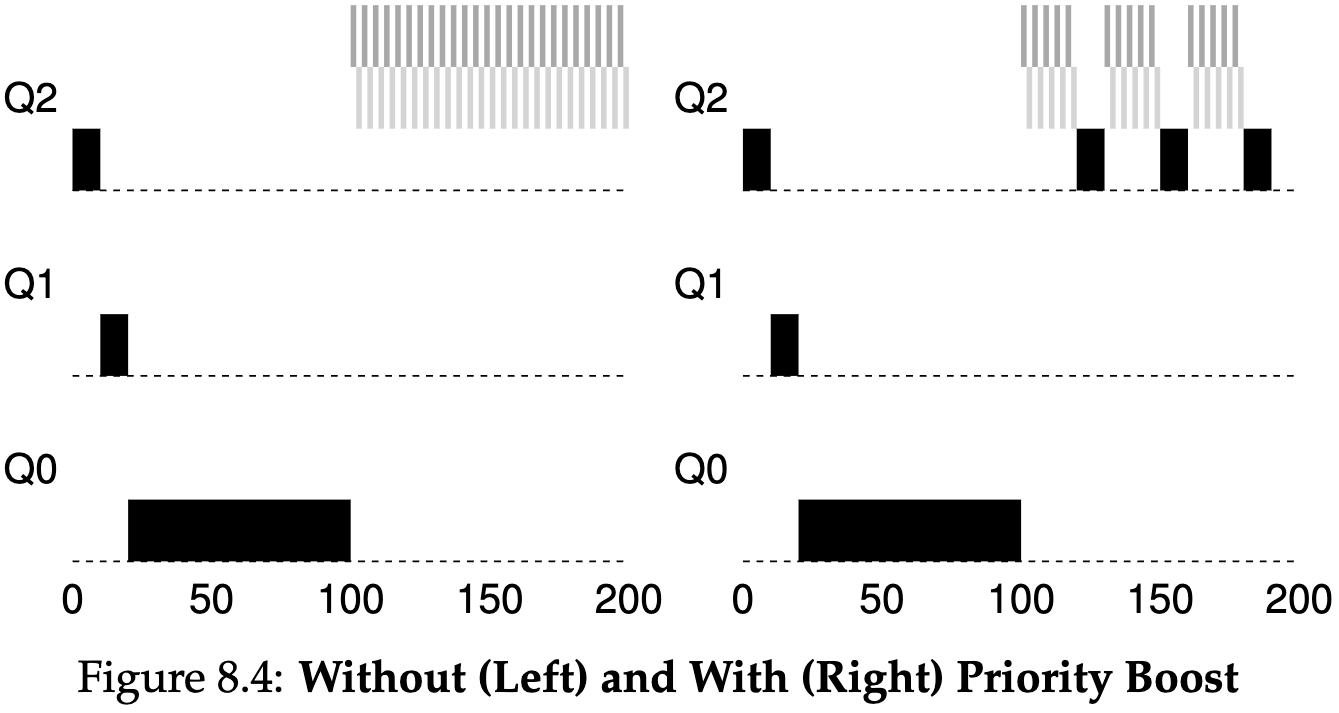
\includegraphics[width=1.1\linewidth]{figs/chapter-8/figure-8.4.png}
            \caption*{Source: chapter page 7.}
            \label{fig:figure-8.4}
        \end{figure}
    \end{columns}
\end{frame}

%------------------------------------------------

\begin{frame}{Attempt \#3: Better Accounting}
    \begin{itemize}
        \item Rules 4a and 4b allow processes to game the scheduler.
        \item The solution is to track the \textbf{total CPU time used at each level}.
        \item Giving up the CPU for I/O no longer resets the allotment.
    \end{itemize}

    \begin{block}{Revised Rule 4}
        Once a job uses up its time allotment at a given level,
        regardless of how many times it has given up the CPU,
        its priority is reduced.
    \end{block}
\end{frame}

%------------------------------------------------

\begin{frame}{Preventing Scheduler Gaming}
    \begin{columns}
        \column{0.45\textwidth}
        \begin{itemize}
            \item Old rules:
            \begin{itemize}
                \item I/O could be used to remain at high priority.
            \end{itemize}

            \item Better accounting:
            \begin{itemize}
                \item CPU usage is accumulated.
                \item The process eventually moves down the queues.
            \end{itemize}
        \end{itemize}

        \column{0.55\textwidth}
        \begin{figure}
            \centering
            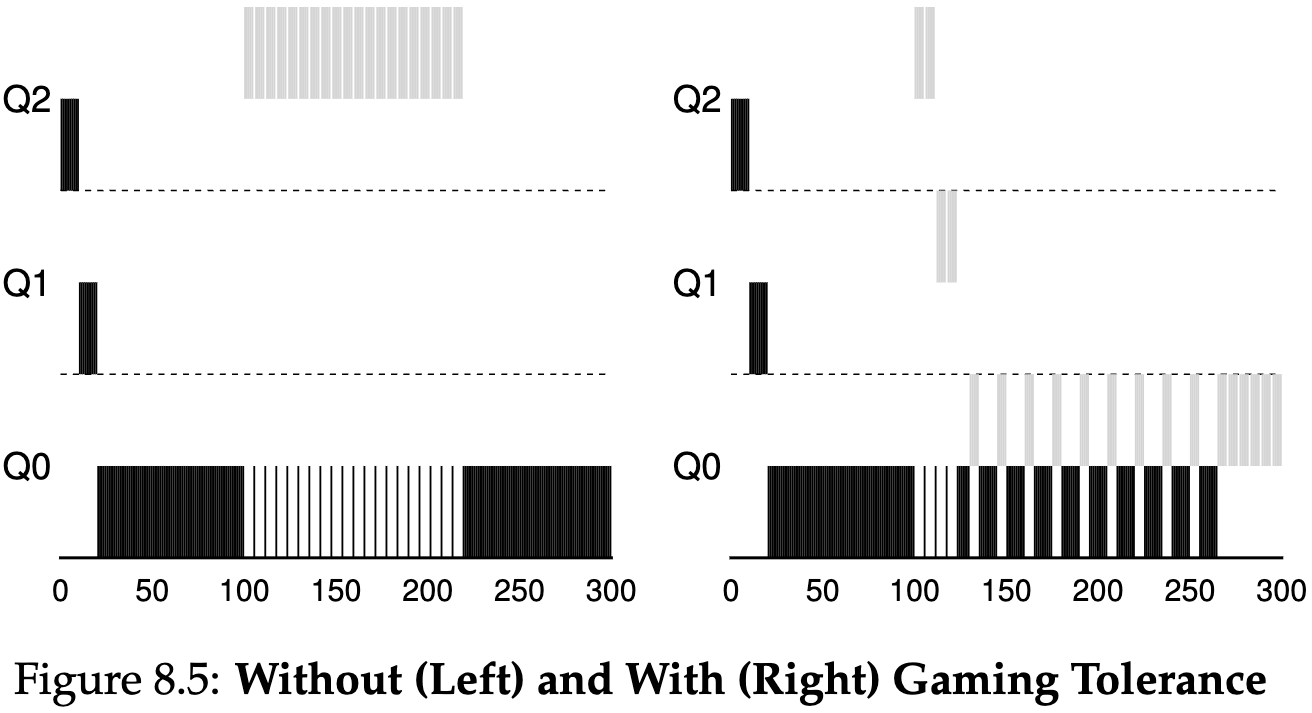
\includegraphics[width=1.1\linewidth]{figs/chapter-8/figure-8.5.png}
            \caption*{Source: chapter page 8.}
            \label{fig:figure-8.5}
        \end{figure}
    \end{columns}
\end{frame}

%------------------------------------------------

\begin{frame}{Tuning MLFQ}
    \begin{itemize}
        \item Important parameters include:
        \begin{itemize}
            \item number of queues;
            \item time slice per queue;
            \item allotment per priority level;
            \item frequency of priority boosts.
        \end{itemize}

        \item High-priority queues usually use \textbf{short time slices}.
        \item Low-priority queues usually use \textbf{longer time slices}.
        \item Interactive jobs benefit from quick switching.
        \item CPU-bound jobs benefit from longer uninterrupted execution.
    \end{itemize}
\end{frame}

%------------------------------------------------

\begin{frame}{Lower Priority, Longer Quanta}
    \begin{columns}
        \column{0.45\textwidth}
        \begin{itemize}
            \item Example:
            \begin{itemize}
                \item highest queue: 10-ms time slice;
                \item middle queue: 20-ms time slice;
                \item lowest queue: 40-ms time slice.
            \end{itemize}
        \end{itemize}

        \column{0.55\textwidth}
        \begin{figure}
            \centering
            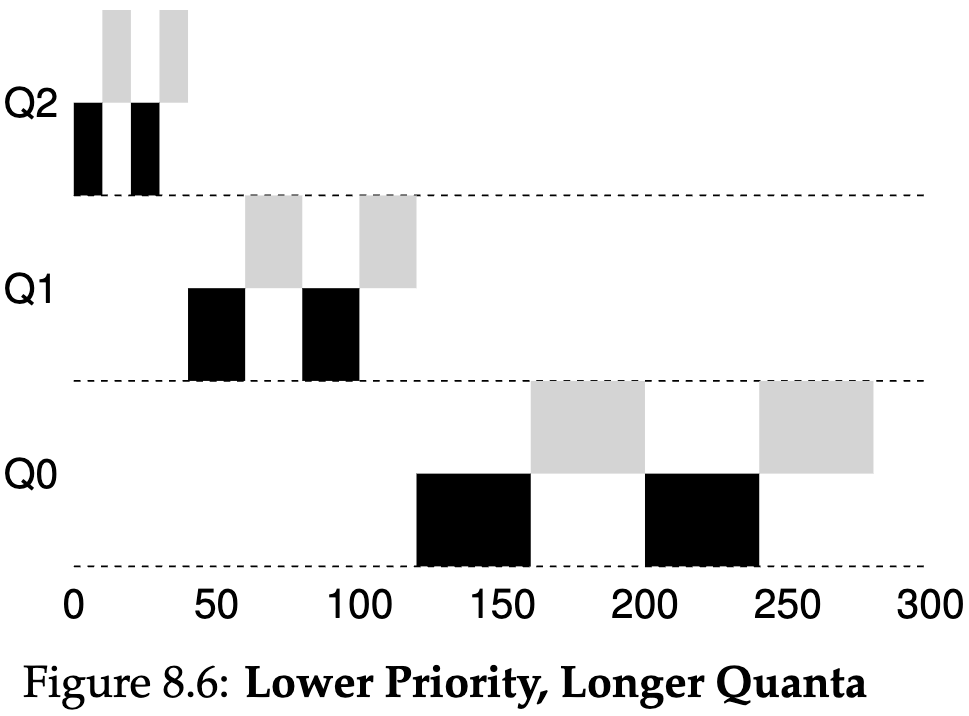
\includegraphics[width=1.1\linewidth]{figs/chapter-8/figure-8.6.png}
            \caption*{Source: chapter page 9.}
            \label{fig:figure-8.6}
        \end{figure}
    \end{columns}
\end{frame}

%------------------------------------------------

\begin{frame}{MLFQ in Real Systems}
    \begin{itemize}
        \item Different systems implement variations of MLFQ.
        \item Solaris Time-Sharing (TS):
        \begin{itemize}
            \item configurable priority tables;
            \item 60 queues in the default configuration;
            \item increasing time-slice lengths at lower priorities;
            \item periodic priority boosts.
        \end{itemize}

        \item FreeBSD uses mathematical formulas based on CPU usage.
        \item Some systems reserve the highest priority levels for OS work.
        \item Utilities such as \texttt{nice} allow users to provide scheduling advice.
    \end{itemize}
\end{frame}

%------------------------------------------------

\begin{frame}{MLFQ: Final Rules}
    \small
    \begin{enumerate}
        \item If Priority(A) $>$ Priority(B), A runs.
        \item If Priority(A) = Priority(B), A and B run in Round Robin.
        \item New jobs enter the system at the highest priority.
        \item Once a job uses its time allotment at a level, its priority is reduced.
        \item After some period $S$, all jobs are moved to the highest-priority queue.
    \end{enumerate}
\end{frame}

%------------------------------------------------

\begin{frame}{Summary}
    \begin{itemize}
        \item MLFQ uses multiple priority queues and feedback from job behavior.
        \item It does not require a priori knowledge of job length.
        \item Short and interactive jobs tend to remain at high priority.
        \item CPU-intensive jobs gradually move to lower-priority queues.
        \item Priority boosts prevent starvation and adapt to behavioral changes.
        \item Better accounting prevents jobs from gaming the scheduler.
        \item MLFQ combines good responsiveness with progress for long-running jobs.
    \end{itemize}
\end{frame}

%------------------------------------------------
%------------------------------------------------
\section{Lottery Scheduling}
%------------------------------------------------

\begin{frame}{Proportional-Share Scheduling}
    \begin{itemize}
        \item Proportional-share schedulers focus on \textbf{fair CPU allocation}.
        \item Instead of optimizing turnaround or response time, the goal is to:
        \begin{itemize}
            \item guarantee that each job receives a certain percentage of CPU time.
        \end{itemize}
        \item Lottery scheduling is an early and influential approach.
    \end{itemize}

    \begin{block}{The Crux}
        How can we design a scheduler to share the CPU proportionally?
    \end{block}
\end{frame}

%------------------------------------------------

\begin{frame}{Lottery Scheduling}
    \begin{itemize}
        \item Lottery scheduling uses \textbf{randomness} to select the next process.
        \item Each process receives a number of \textbf{tickets}.
        \item Tickets represent a process's share of the CPU.
        \item A lottery is held periodically, typically once per time slice.
        \item The process holding the winning ticket runs next.
    \end{itemize}
\end{frame}

%------------------------------------------------

\begin{frame}{Tickets Represent CPU Share}
    \begin{itemize}
        \item Suppose:
        \begin{itemize}
            \item Process A has 75 tickets.
            \item Process B has 25 tickets.
        \end{itemize}

        \item Desired CPU allocation:
        \[
            A = 75\%, \qquad B = 25\%
        \]

        \item The scheduler randomly selects one ticket among all available tickets.
        \item Allocation is \textbf{probabilistic}, not deterministic.
        \item Over longer execution periods, the obtained proportions tend to approach
        the desired shares.
    \end{itemize}
\end{frame}

%------------------------------------------------

\begin{frame}{Why Randomness?}
    \begin{itemize}
        \item Randomized scheduling has several useful properties:
        \begin{itemize}
            \item avoids some pathological corner cases;
            \item requires little per-process state;
            \item can make scheduling decisions quickly.
        \end{itemize}
        \item Lottery scheduling only needs:
        \begin{itemize}
            \item the number of tickets per process;
            \item the total number of tickets;
            \item a random number generator.
        \end{itemize}
    \end{itemize}
\end{frame}

%------------------------------------------------

\begin{frame}{Ticket Mechanisms}
    \begin{description}
        \item[Ticket Currency]
        Users can distribute tickets among their own jobs using a local currency,
        which is converted into a global ticket value.

        \item[Ticket Transfer]
        A process can temporarily transfer its tickets to another process.

        \item[Ticket Inflation]
        A process can temporarily increase or decrease its number of tickets
        in environments where processes trust one another.
    \end{description}
\end{frame}

%------------------------------------------------

\begin{frame}{Lottery Scheduling: Implementation}
    \begin{columns}
        \column{0.48\textwidth}
        \begin{itemize}
            \item Keep runnable processes in a data structure such as a list.
            \item Generate a random winning ticket.
            \item Traverse the process list while accumulating ticket counts.
            \item The process whose accumulated count exceeds the winning ticket
            is selected.
        \end{itemize}

        \column{0.52\textwidth}
        \begin{figure}
            \centering
            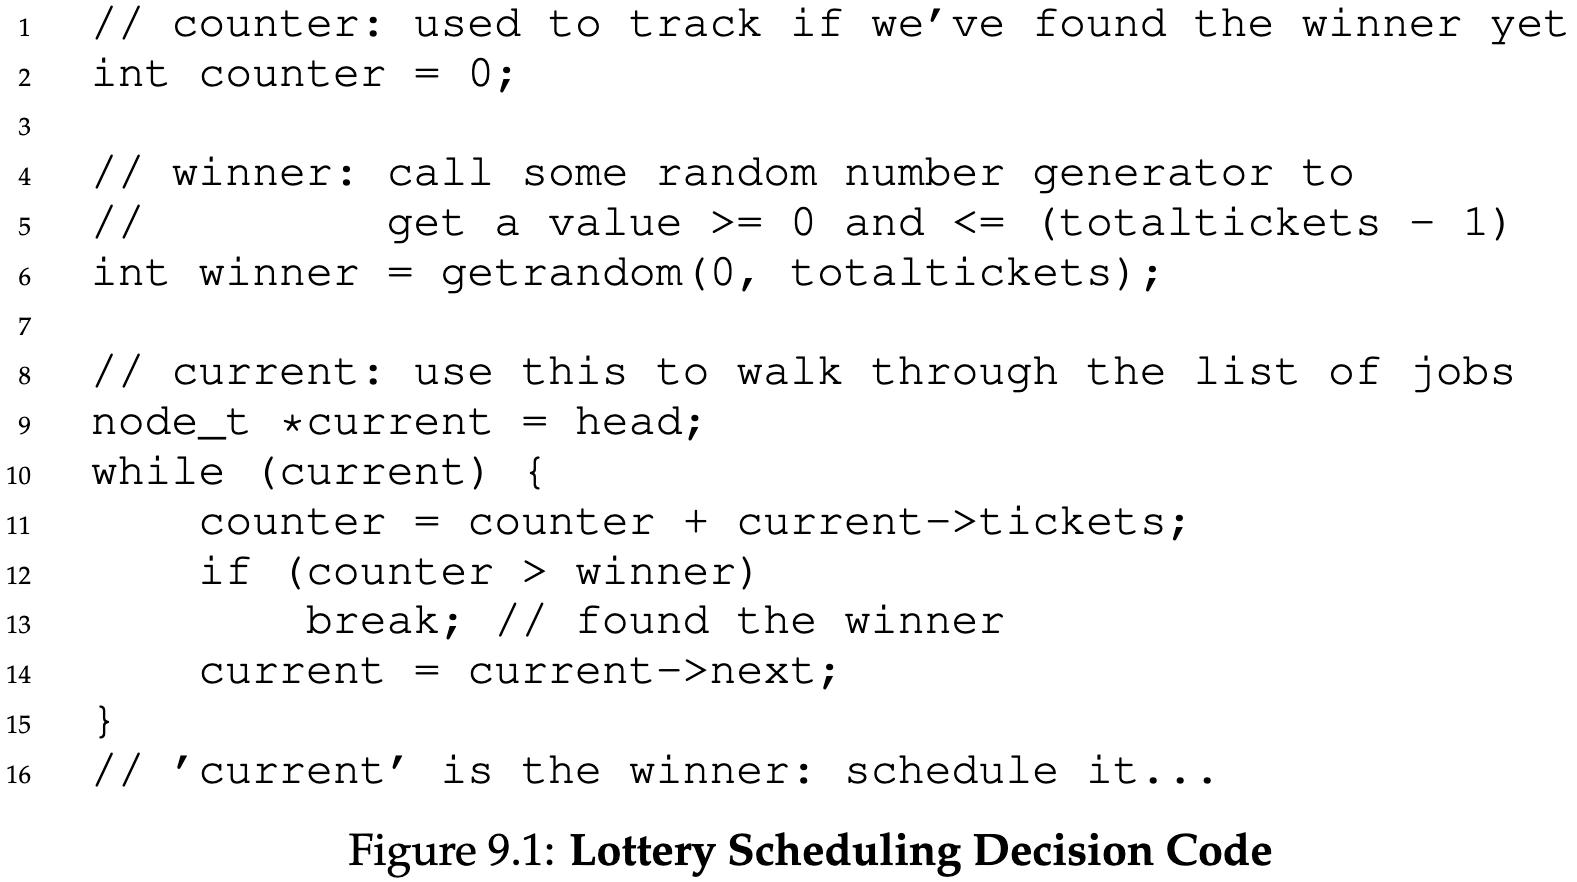
\includegraphics[width=1.1\linewidth]{figs/chapter-9/figure-9.1.png}
            \caption*{Source: chapter page 4.}
            \label{fig:figure-9.1}
        \end{figure}
    \end{columns}
\end{frame}

%------------------------------------------------

\begin{frame}{Lottery Scheduling Example}
    \begin{itemize}
        \item Consider three jobs:
        \begin{itemize}
            \item A: 100 tickets;
            \item B: 50 tickets;
            \item C: 250 tickets.
        \end{itemize}

        \item Total number of tickets:
        \[
            100 + 50 + 250 = 400
        \]

        \item If the winning ticket is 300:
        \begin{itemize}
            \item A covers tickets up to 100;
            \item A+B cover tickets up to 150;
            \item A+B+C cover tickets up to 400.
        \end{itemize}

        \item Therefore, process C wins the lottery.
    \end{itemize}
\end{frame}

%------------------------------------------------

\begin{frame}{Lottery Scheduling Fairness}
    \begin{columns}
        \column{0.48\textwidth}
        \begin{itemize}
            \item Consider two jobs with:
            \begin{itemize}
                \item equal ticket allocations;
                \item equal runtime $R$.
            \end{itemize}

            \item Fairness is defined as:
            \[
                F =
                \frac{\text{completion time of first job}}
                     {\text{completion time of second job}}
            \]

            \item A perfectly fair result gives:
            \[
                F = 1
            \]
        \end{itemize}

        \column{0.52\textwidth}
        \begin{figure}
            \centering
            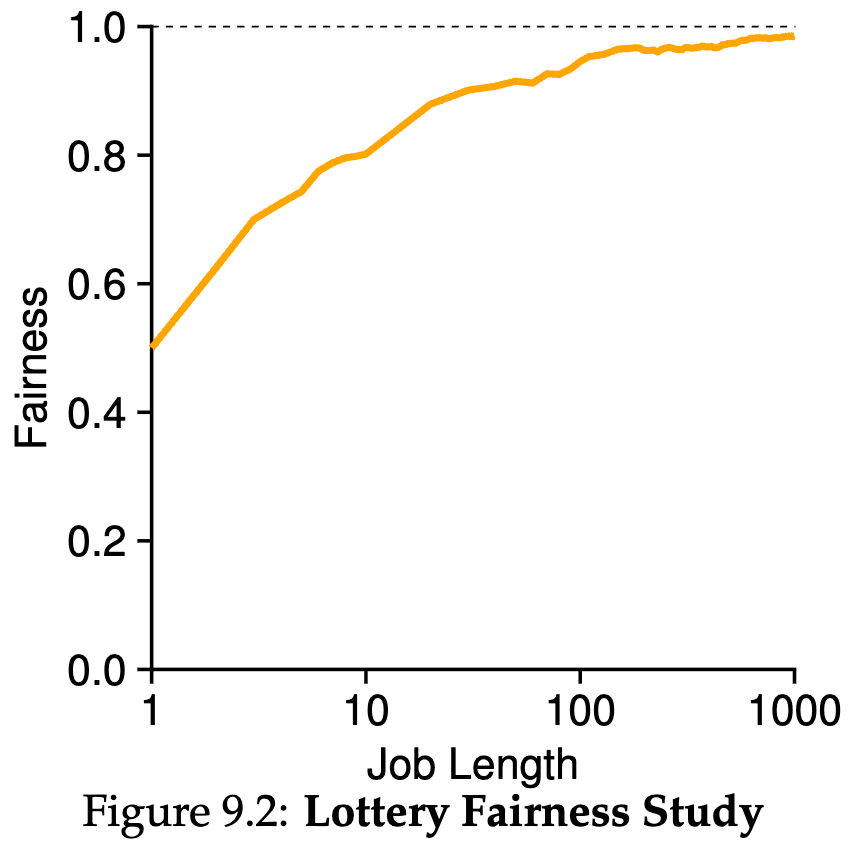
\includegraphics[width=1.1\linewidth]{figs/chapter-9/figure-9.2.png}
            \caption*{Source: chapter page 5.}
            \label{fig:figure-9.2}
        \end{figure}
    \end{columns}
\end{frame}

%------------------------------------------------

\begin{frame}{Fairness Over Time}
    \begin{itemize}
        \item For short jobs, lottery scheduling may produce significant unfairness.
        \item Randomness can cause one job to finish substantially earlier than another.
        \item As job length increases:
        \begin{itemize}
            \item more lotteries are performed;
            \item average fairness approaches the desired result.
        \end{itemize}
        \item Thus, lottery scheduling achieves proportional fairness
        \textbf{probabilistically over time}.
    \end{itemize}
\end{frame}

%------------------------------------------------

\begin{frame}{How Should Tickets Be Assigned?}
    \begin{itemize}
        \item The behavior of lottery scheduling strongly depends on ticket allocation.
        \item One possibility is to give users a fixed number of tickets.
        \item Users may then distribute their tickets among their jobs.
        \item However, the general \textbf{ticket-assignment problem} remains open.
    \end{itemize}
\end{frame}

%------------------------------------------------

\begin{frame}{Stride Scheduling}
    \begin{itemize}
        \item Stride scheduling provides a \textbf{deterministic} approach
        to proportional-share scheduling.
        \item Each process has:
        \begin{itemize}
            \item a number of tickets;
            \item a \textbf{stride};
            \item a \textbf{pass value}.
        \end{itemize}

        \item Stride is inversely proportional to the number of tickets:
        \[
            stride_i = \frac{\text{large constant}}{tickets_i}
        \]

        \item Processes with more tickets therefore have smaller strides.
    \end{itemize}
\end{frame}

%------------------------------------------------

\begin{frame}{Stride Scheduling: Basic Operation}
    \begin{enumerate}
        \item Select the process with the \textbf{lowest pass value}.
        \item Run it for one quantum.
        \item Update its pass value:
        \[
            pass_i = pass_i + stride_i
        \]
        \item Return the process to the scheduling queue.
    \end{enumerate}

    \begin{block}{Main Difference}
        Lottery scheduling achieves proportions probabilistically,
        whereas stride scheduling achieves them deterministically.
    \end{block}
\end{frame}

%------------------------------------------------

\begin{frame}{Stride Scheduling Example}
    \begin{columns}
        \column{0.42\textwidth}
        \begin{itemize}
            \item Tickets:
            \begin{itemize}
                \item A: 100
                \item B: 50
                \item C: 250
            \end{itemize}

            \item Using 10,000 as the constant:
            \[
            \begin{aligned}
                stride_A &= 100\\
                stride_B &= 200\\
                stride_C &= 40
            \end{aligned}
            \]

            \item The process with the lowest pass runs next.
        \end{itemize}

        \column{0.58\textwidth}
        \begin{figure}
            \centering
            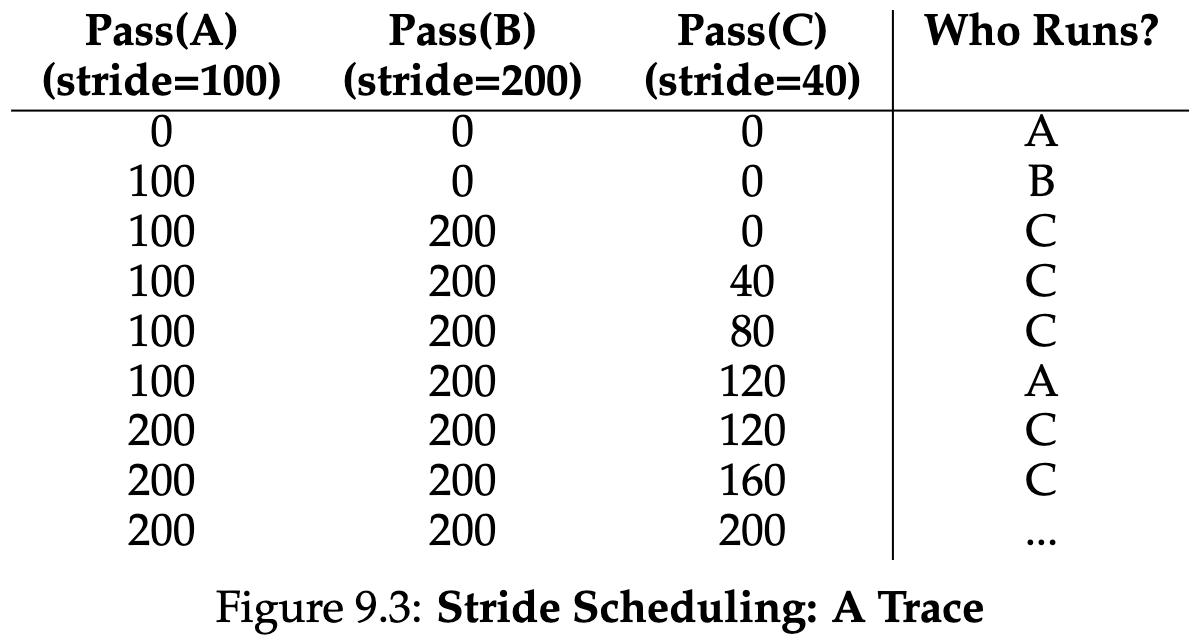
\includegraphics[width=1.1\linewidth]{figs/chapter-9/figure-9.3.png}
            \caption*{Source: chapter page 7.}
            \label{fig:figure-9.3}
        \end{figure}
    \end{columns}
\end{frame}

%------------------------------------------------

\begin{frame}{Lottery vs. Stride Scheduling}
    \begin{itemize}
        \item \textbf{Lottery Scheduling}
        \begin{itemize}
            \item probabilistic;
            \item simple;
            \item little global state;
            \item easy to incorporate new processes.
        \end{itemize}

        \item \textbf{Stride Scheduling}
        \begin{itemize}
            \item deterministic;
            \item achieves exact proportions at the end of scheduling cycles;
            \item requires maintaining pass values.
        \end{itemize}

        \item Adding a new process is more complicated in stride scheduling
        because an appropriate initial pass value must be chosen.
    \end{itemize}
\end{frame}

%------------------------------------------------

\begin{frame}{Linux Completely Fair Scheduler}
    \begin{itemize}
        \item The Completely Fair Scheduler (CFS) implements fair-share scheduling
        using a different approach.
        \item Main goals:
        \begin{itemize}
            \item fairness;
            \item efficiency;
            \item scalability.
        \end{itemize}
        \item CFS attempts to spend very little CPU time making scheduling decisions.
        \item Its basic mechanism is called \textbf{virtual runtime}
        (\texttt{vruntime}).
    \end{itemize}
\end{frame}

%------------------------------------------------

\begin{frame}{CFS: Virtual Runtime}
    \begin{itemize}
        \item Each running process accumulates \texttt{vruntime}.
        \item In the simplest case, \texttt{vruntime} increases with physical runtime.
        \item CFS selects the runnable process with the
        \textbf{lowest \texttt{vruntime}}.
        \item The objective is to keep CPU execution distributed fairly among processes.
    \end{itemize}

    \begin{block}{Scheduling Decision}
        Run the process that has received the least virtual CPU time.
    \end{block}
\end{frame}

%------------------------------------------------

\begin{frame}{CFS: Dynamic Time Slices}
    \begin{itemize}
        \item CFS uses \texttt{sched\_latency} to determine a target scheduling period.
        \item With $n$ runnable processes:
        \[
            time\_slice =
            \frac{\texttt{sched\_latency}}{n}
        \]

        \item Example:
        \begin{itemize}
            \item \texttt{sched\_latency} = 48 ms;
            \item $n=4$ processes;
            \item each process receives approximately 12 ms.
        \end{itemize}
    \end{itemize}
\end{frame}

%------------------------------------------------

\begin{frame}{CFS: Simple Example}
    \begin{columns}
        \column{0.42\textwidth}
        \begin{itemize}
            \item Four jobs initially share the CPU.
            \item Each receives a 12-ms time slice.
            \item After C and D finish:
            \begin{itemize}
                \item only A and B remain;
                \item each receives a 24-ms time slice.
            \end{itemize}
            \item Time slices therefore change dynamically.
        \end{itemize}

        \column{0.58\textwidth}
        \begin{figure}
            \centering
            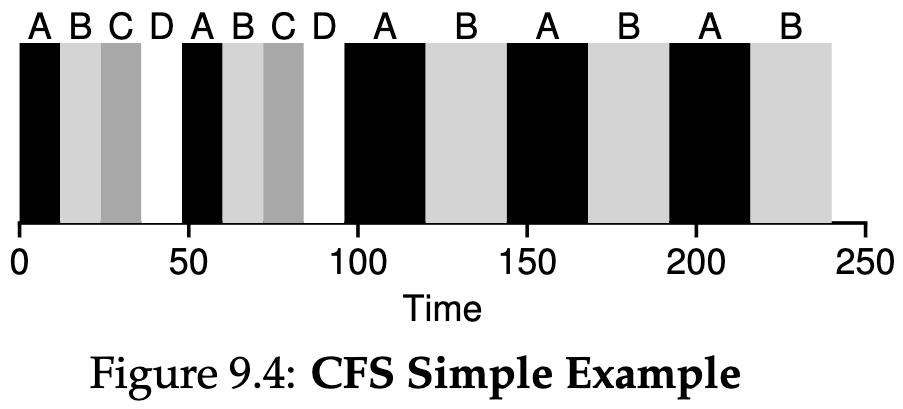
\includegraphics[width=1.1\linewidth]{figs/chapter-9/figure-9.4.png}
            \caption*{Source: chapter page 7.}
            \label{fig:figure-9.4}
        \end{figure}
    \end{columns}
\end{frame}

%------------------------------------------------

\begin{frame}{CFS: Minimum Granularity}
    \begin{itemize}
        \item With many runnable processes, calculated time slices may become very small.
        \item Very small slices increase context-switch overhead.
        \item CFS therefore uses \texttt{min\_granularity}.
        \item A typical value discussed in the chapter is 6 ms.
        \item CFS will not assign a time slice smaller than this value.
    \end{itemize}

    \begin{block}{Trade-off}
        CFS balances short-term fairness against scheduling and
        context-switching overhead.
    \end{block}
\end{frame}

%------------------------------------------------

\begin{frame}{CFS: Weighting and Niceness}
    \begin{itemize}
        \item CFS supports different CPU shares through UNIX \textbf{nice values}.
        \item Nice values range from:
        \[
            -20 \ \text{to}\ +19
        \]

        \item Negative nice values imply higher priority.
        \item Positive nice values imply lower priority.
        \item Nice values are mapped to numerical \textbf{weights}.
    \end{itemize}

    \[
        time\_slice_k =
        \frac{weight_k}
        {\sum_{i=0}^{n-1} weight_i}
        \cdot sched\_latency
    \]
\end{frame}

%------------------------------------------------

\begin{frame}{Weighted Virtual Runtime}
    \begin{itemize}
        \item CFS also adjusts the rate at which \texttt{vruntime} increases.
        \item Processes with larger weights accumulate virtual runtime more slowly.
    \end{itemize}

    \[
        vruntime_i =
        vruntime_i +
        \frac{weight_0}{weight_i}
        \cdot runtime_i
    \]

    \begin{itemize}
        \item Higher-priority processes therefore remain eligible to run
        more frequently.
    \end{itemize}
\end{frame}

%------------------------------------------------

\begin{frame}{CFS and Red-Black Trees}
    \begin{columns}
        \column{0.48\textwidth}
        \begin{itemize}
            \item CFS must efficiently find the process with the smallest
            \texttt{vruntime}.
            \item Runnable processes are stored in a \textbf{red-black tree}.
            \item Processes are ordered according to \texttt{vruntime}.
            \item Important operations take:
            \[
                O(\log n)
            \]
            \item This scales better than linear lists.
        \end{itemize}

        \column{0.52\textwidth}
        \begin{figure}
            \centering
            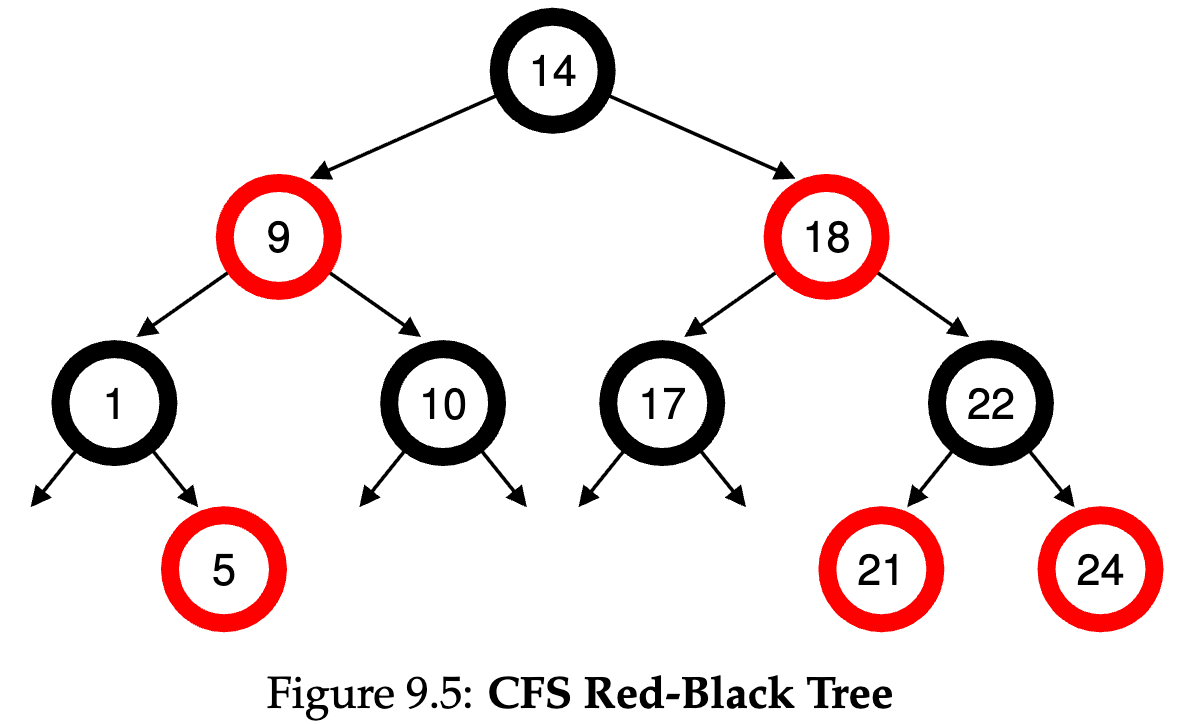
\includegraphics[width=1.1\linewidth]{figs/chapter-9/figure-9.5.png}
            \caption*{Source: chapter page 11.}
            \label{fig:figure-9.5}
        \end{figure}
    \end{columns}
\end{frame}

%------------------------------------------------

\begin{frame}{CFS and Sleeping Processes}
    \begin{itemize}
        \item Sleeping processes are removed from the red-black tree.
        \item A long-sleeping process may wake with a much smaller
        \texttt{vruntime} than active processes.
        \item Without correction, it could monopolize the CPU while catching up.
        \item CFS handles this by setting its \texttt{vruntime} to the minimum
        value currently found in the tree.
        \item This avoids starvation of other runnable processes.
    \end{itemize}
\end{frame}

%------------------------------------------------

\begin{frame}{Proportional-Share Scheduling: Summary}
    \begin{itemize}
        \item \textbf{Lottery Scheduling}
        \begin{itemize}
            \item uses tickets and randomness;
            \item achieves proportional allocation probabilistically.
        \end{itemize}

        \item \textbf{Stride Scheduling}
        \begin{itemize}
            \item uses stride and pass values;
            \item provides deterministic proportional allocation.
        \end{itemize}

        \item \textbf{CFS}
        \begin{itemize}
            \item uses virtual runtime and dynamic time slices;
            \item uses weights to support different CPU shares;
            \item uses red-black trees for efficient scheduling.
        \end{itemize}
    \end{itemize}
\end{frame}

%------------------------------------------------

\begin{frame}{Final Remarks}
    \begin{itemize}
        \item Fair-share scheduling does not solve every scheduling problem.
        \item Important challenges remain:
        \begin{itemize}
            \item interaction with I/O;
            \item assigning tickets or priorities appropriately.
        \end{itemize}
        \item Proportional sharing can be effective when explicit resource
        allocation is desirable, such as in virtualized environments.
        \item As of Linux 6.6, Linux adopted the
        \textbf{Earliest Eligible Virtual Deadline First (EEVDF)}
        scheduling approach as the default.
    \end{itemize}
\end{frame}

%------------------------------------------------

\begin{frame}[allowframebreaks]
\nocite{*}
\printbibliography
\end{frame}

\begin{frame}{}
  \centering \Large
  \textbf{? \& | !}
\end{frame}

\end{document}
